\documentclass[11pt]{article}
\usepackage[letterpaper,margin=1in]{geometry}
\usepackage[T1]{fontenc}
\usepackage{amsmath,amsthm}
\usepackage{newtxtext,newtxmath}
\usepackage{microtype,graphicx,booktabs,tabularx,array}
\usepackage[numbers,sort&compress]{natbib}
\usepackage{enumitem,placeins}
\usepackage{xcolor}
\definecolor{linkblue}{RGB}{24,69,102}
\usepackage[colorlinks=true,allcolors=linkblue]{hyperref}
\usepackage[nameinlink,noabbrev]{cleveref}
\crefname{proposition}{proposition}{propositions}
\crefname{corollary}{corollary}{corollaries}
\crefname{lemma}{lemma}{lemmas}
\crefname{assumption}{assumption}{assumptions}
\hypersetup{pdftitle={Nonlocal heat-flux closure across collision models},
 pdfsubject={Variational bounds, exact responses, and limits of transfer},
 pdfkeywords={plasma, kinetic closure, BGK, Dougherty, Landau, electron heat flux}}
\widowpenalty=10000
\clubpenalty=10000
\setlist{nosep,leftmargin=*}
\setlength{\emergencystretch}{2em}
\setlength{\parskip}{3pt}
\newcommand{\dd}{\,\mathrm d}
\newcommand{\av}[1]{\left\langle #1\right\rangle}
\newcommand{\D}{\mathcal D}
\newcommand{\HH}{\mathcal H}
\newcommand{\A}{\mathcal A}
\newcommand{\F}{\kappa_{\mathrm F}}
\newcommand{\He}{\mathrm{He}}
\newcommand{\sgn}{\operatorname{sgn}}
\newcommand{\Real}{\operatorname{Re}}
\newcommand{\Imag}{\operatorname{Im}}
\newcommand{\RR}{\mathbb R}
\newcommand{\N}{\mathcal N}
\newcommand{\kap}{\kappa}
\newcommand{\thr}{\mathrm{th}}
\newcommand{\pot}{\mathrm{pot}}
\newcommand{\Qth}{\mathcal Q^{\thr}}
\newcommand{\Pth}{\mathcal P^{\thr}}
\newcommand{\norm}[1]{\left\|#1\right\|}
\newcommand{\nstar}[1]{\left\|#1\right\|_*}
\newcommand{\dual}[1]{\left\langle #1,\Lambda^+ #1\right\rangle}
\newtheorem{theorem}{Theorem}[section]
\newtheorem{proposition}[theorem]{Proposition}
\newtheorem{lemma}[theorem]{Lemma}
\newtheorem{corollary}[theorem]{Corollary}
\theoremstyle{definition}
\newtheorem{assumption}[theorem]{Assumption}
\theoremstyle{remark}
\newtheorem{remark}[theorem]{Remark}
\numberwithin{equation}{section}
\title{\bfseries Nonlocal heat-flux closure across collision models:\\
variational bounds, exact responses,\\ and limits of transfer}
\author{}
\date{17 November 2026}
\begin{document}
\maketitle
\vspace{-1.5em}
\begin{abstract}
A kinetic heat-flux closure can recover both the local and the
collisionless limits and still be undetermined at intermediate
collisionality. How much freedom is left, and how do we test for it?
We work with linear perturbations of a Maxwellian, and we define the
closure as the quasi-static response of the kinetic equation to a
specified drive.
For a potential force in one velocity dimension, a conserving, symmetric
collision operator admits a pair of dual variational principles that
bracket the exact response and give $\F/(1+Kk^2)\leq\chi(k)\leq\F$.
Under stated solvability hypotheses, $K$ is exactly the leading
coefficient of the conductivity deficit. Constant-frequency BGK and the
conserving Dougherty operator give explicit reference formulas, including
both the collisional and the collisionless limits.
Three velocity dimensions are harder. The potential-driven temperature
response picks up a stress cross term, and what survives is a set of
two-sided small-wavenumber bounds, the leading coefficient, and the
positivity criterion $k^2\F\eta<3$. Nothing more survives in general:
for relaxation operators with a slow stress $\chi>\F$, and with a slow
heat flux as well $\chi<0$, so the constant $3$ cannot be raised above
$25/8$. Weighted coercivity estimates make
these rigorous for like-particle Landau--Coulomb collisions. For that
operator we also prove the collisionless limit
$|k|\chi\to3\sqrt{2/\pi}$, by matching variational bounds built on an
Airy-type boundary layer, and with it positivity at all sufficiently
large wavenumbers.
Changing the drive removes the obstruction. For an isotropic heating
source the temperature response is a diagonal entry of the resolvent, and
$\kap/(1+K_\thr k^2)\leq\chi_\thr(k)\leq\kap$ holds at every wavenumber for
every symmetric, nonnegative collision operator whose kernel contains the
density and energy invariants. Momentum conservation is not among the
hypotheses, so the result covers electron--electron Landau collisions
together with pitch-angle scattering on ions of charge $Z$, with $\kap$
the conductivity at zero current. More is true: $\chi_\thr$ is a
Stieltjes function of $k^2$. It decreases in $|k|$, its real-space kernel
is a positive mixture of exponentials, and the two-sided bound is the
first of a family of Pad\'e bounds. For both operators we prove the
solvability that these theorems require, and the collisionless limit
$|k|\chi_\thr\to\tfrac95\sqrt{2/\pi}$, which does not depend on $Z$. The two drives share the conductivity
but not the deficit: for Dougherty the leading coefficients are
$2/(15\nu^2)$ and $16/(45\nu^2)$.
Polynomial Galerkin calculations give $\F/\tau\simeq3.9502$ and
$K/\tau^2\simeq22.35$ for like-particle Landau collisions, a leading
deficit approximately $7.45$ times that of the Dougherty operator at
matched conductivity. They reproduce Braginskii's electron coefficients
at low degree, and they give a normalized deficit $K_\thr/\kap^2$ that
grows roughly linearly in $Z$, from about $4.3$ at $Z=1$ to $96$ at
$Z=64$. We prove the linear law: the slope, $1.4305$, is the solution of
a radial like-particle problem, and at large $Z$ the whole response
converges, with two-sided bounds, to a diffusive limit that depends on
the wavenumber only through $\sqrt Z\,k\lambda_e$. Matching the
conductivity does not match the closure.
Whether matching the static response does depends on the dynamics. The
exact closure for data in the retained moments is a convolution in time
with a positive-real kernel whose zero-frequency value is the quasi-static
response, and the error of the quasi-static closure is bounded by the
variation of that kernel over the frequencies the closed model excites. In a
one-dimensional model coupled to sound waves, the exact quasi-static
closure has transient errors of up to $34\%$. In the quasi-neutral decay
of an electron temperature perturbation it stays within $2\%$ for $Z=1$
at $|k|\lambda_e\leq0.3$, where Spitzer--H\"arm conduction is off by
$42\%$.
These results are analytic tests for learned and classical closures
alike. They are not a general constitutive law. The like-particle
collisionless limits come with the rate $O(|k|^{-2/3}\log|k|)$ and an
inexplicit constant, the electron limit with no rate, and the Landau and
electron theorems rest on published coercivity estimates for the Landau
operator, which we cite and do not reprove.
\end{abstract}
\noindent\textbf{Keywords:} kinetic closure; nonlocal transport; BGK;
Dougherty; Landau operator; electron--ion collisions;
Spitzer--H\"arm conductivity; variational bounds; reduced models.

\section{Introduction}

The local heat law $q=-\F\,\partial_xT$ replaces all of the unresolved
velocity dependence of a kinetic distribution with a single transport
coefficient. It works when there is a separation of time and length
scales: collisions must equilibrate the heat-carrying part of the
distribution before those particles see much variation in the resolved
fields. Plasma transport strains this separation for three reasons.
Collision rates depend strongly on speed, phase mixing competes with
relaxation, and a scalar temperature need not capture the anisotropy that
streaming generates.

Different lines of work address different parts of this problem: the
classical conductivity calculation of Spitzer and H\"arm
\cite{SpitzerHarm1953}, nonlocal transport kernels
\cite{LMV1983}, and fluid representations of Landau damping
\cite{HP1990,Snyder1997,Hunana2019}.
At arbitrary collisionality, moment-based integral closures can represent
heat flow together with viscosity and friction \cite{JiHeld2014}.
Comparisons against kinetic solvers show, however, that performance
depends on the drive, the temperature contrast, and the collision
physics~\cite{Brodrick2017}. The lesson we take from this literature is
that an interpolant fitted to two asymptotic limits needs an independent
test in the regime between them.

We develop such tests here, for a response that is deliberately
restricted and mathematically precise. The full state is a linearized
distribution $h$. We retain the density, velocity, and temperature, and
we discard the heat flux, the stress, and all higher moments. The
classical reduced operator is the linear Euler system with
Chapman--Enskog transport. We isolate the heat-flux defect through a
Fourier multiplier $\chi(k)$, which we obtain by slowly forcing the
kinetic system away from equilibrium. The advantage of this construction
is that there is no ambiguity about what is being compared. What it does
not do is assume that an instantaneous function of temperature closes
every kinetic trajectory. (It does not; \cref{sec:embedded} has an
example.)

Our analysis has five parts. First, we use conservation and a parity
decomposition to convert the one-dimensional stationary problem into a
pair of dual quadratic optimization problems. These give positivity and
two-sided bounds at every nonzero wavenumber, and they do not require a
closed-form inverse of the collision operator. Second, we work out the
BGK and Dougherty models explicitly, so that both the analysis and the
computations have exact responses to check against. Third, we keep the
stress contribution in three dimensions and show exactly where the
one-dimensional positivity argument breaks down. The breakdown is real:
explicit relaxation operators violate the Fourier upper bound and
positivity (\cref{sec:ce}). A weighted functional
setting for Landau--Coulomb collisions, together with reproducible
Galerkin calculations, connects these estimates to a more realistic
collision kernel. For that kernel we also prove the collisionless limit
(\cref{thm:airy}): the resonant layer has width $(d/k)^{1/3}$, with $d$
the local velocity diffusion coefficient, and the limiting response does
not depend on $d$. The limit is approached at the rate
$O(|k|^{-2/3}\log|k|)$ (\cref{thm:rate}).

The last two parts move toward the problem that plasma transport codes
actually close, which is electron heat flux. Fourth, we replace the
potential force by an isotropic heating source (\cref{sec:th-thermal}).
The heat flux is then exactly $1/(ik)$ per unit heating, the current
vanishes, and the temperature response is a positive quadratic form. The
three-dimensional problem becomes as clean as the one-dimensional one:
we obtain bounds at every wavenumber and the sharp leading coefficient
with an $O(k^4)$ remainder, and for like-particle Landau collisions this
gives the positivity and the Fourier upper bound that are open for the
potential drive. The response is moreover a Stieltjes function of $k^2$
(\cref{thm:stieltjes}), which makes the exact closure a positive
superposition of screened diffusion problems, the form that multigroup
transport models assume. The drive
matters. Both responses are entries of one positive-definite $2\times2$
matrix of parallel and perpendicular temperature responses; they share
the conductivity but not the leading deficit. Fifth, none of the thermal
theorems needs momentum conservation, so they hold for electron--electron
plus electron--ion collisions with the conductivity replaced by its
zero-current value (\cref{sec:th-electron}). For this operator we prove
weighted solvability and the collisionless limit, so the electron closure
is fixed by theorems at both ends of the wavenumber range. At large ion
charge we go further (\cref{thm:largeZ,thm:LZ-limit}): the ions act only
on the anisotropic part of the distribution, the response converges to
that of a radial diffusion problem, and the leading deficit grows
linearly in the charge with an explicit slope. We compute the constants
and the response curves for ion charges from $1$ to $64$, and we test the
closure as an evolution law in the quasi-neutral decay of a temperature
perturbation (\cref{sec:th-numerics}).

Throughout, we compare collision models at fixed conductivity rather than
at fixed nominal collision frequency. Even after this matching, the
small-$k$ coefficient of the conductivity deficit depends strongly on the
collision operator, and the error of the usual harmonic interpolant
changes sign over the intermediate regime that we resolve. Match the two
endpoints, match the local transport coefficient, and you still have not
matched the closure. Electron--ion scattering makes the mismatch larger:
the normalized coefficient grows roughly linearly in the ion charge.

What is new here, and what is not? This paper synthesizes and rederives
a sequence of internal closure notes, with unified conventions, explicit
hypotheses, and numerical evidence that we have reproduced. We do not
claim priority for the underlying response formulas or the variational
techniques; exact solutions of kinetic model equations have a long
history \cite{BGK1954,Dougherty1964,Struchtrup1997}. Our forced-response
closure is also a different object from the invariant
hydrodynamic manifolds and spectral closures of Kogelbauer and Karlin
\cite{KogelbauerKarlin2024,KogelbauerKarlin2025}. A response ratio is
tied to its input. An invariant manifold is a reduction of the
autonomous dynamics.

\section{The response being closed}\label{sec:setting}

\subsection{Units, moments, and the exact hierarchy}

Let $d=1$ or $3$, with one spatial coordinate $x$ and velocity
$v\in\RR^d$. Write $v_x=v$ when $d=1$. The normalized Maxwellian and
average are
\[
 M_d(v)=(2\pi)^{-d/2}e^{-|v|^2/2},
 \qquad \av{b}=\int_{\RR^d}b(v)M_d(v)\dd v.
\]
The perturbation is $f=M_d(1+h)$. Its dimensionless moments are
\begin{equation}
 n=\av h,\quad u=\av{v_xh},\quad
 T=\av{\zeta_d h},\quad q=\av{Q_dh},\qquad
 \zeta_d=\frac{|v|^2-d}{d},\quad
 Q_d=\frac12 v_x(|v|^2-d-2).
 \label{eq:moments}
\end{equation}
Thus $q$ is the \emph{energy flux relative to the local flow}.
A warning about conventions. In one dimension, Landau-fluid
papers often write $q$ for the parallel third central moment, which is
$2q$ in our convention. The Hammett--Perkins coefficient $\sqrt{8/\pi}$
therefore becomes $\sqrt{2/\pi}$ here. The same factor of two applies to
the conductivity, but relative conductivity deficits are unaffected.

To restore units, choose a reference time $t_*$ and
$v_t=\sqrt{T_0/m}$, with temperature measured in energy units.
Set $x_*=v_tt_*$, $v_{\rm phys}=v_tv$,
$t_{\rm phys}=t_*t$, and $k=k_{\rm phys}x_*$.
The dimensional perturbations are
$\delta n=n_0n$, $\delta u=v_tu$, $\delta T=T_0T$ and
$q_{\rm phys}=n_0T_0v_tq$. Consequently
\begin{equation}
 \chi_{\rm phys}=n_0v_t^2t_*\,\chi,\qquad
 \kappa_{\mathrm{F,phys}}=n_0v_t^2t_*\,\F,\qquad
 s=|k|\F=\frac{|k_{\rm phys}|\kappa_{\mathrm{F,phys}}}{n_0v_t}.
 \label{eq:units}
\end{equation}
If a temperature in kelvin is used, the corresponding conductivity includes
$k_B$. All results below use these dimensionless variables; a collision
frequency $\nu$ is understood to include the factor $t_*$.

We consider
\begin{equation}
 \partial_th+v_x\partial_xh+\Lambda h=a(t,x)v_x,\qquad h(0)=0,
 \label{eq:kinetic}
\end{equation}
on the whole line or a periodic domain. The collision operator is real,
self-adjoint and nonnegative in $L^2(M_d)$, conserves mass, momentum and
energy, and commutes with reflection in $v_x$. Its kernel is the
collision-invariant space. In three dimensions we restrict to
axisymmetry about $x$, so this space is
$H=\operatorname{span}\{1,v_x,|v|^2\}$.

The exact retained equations are
\begin{align}
 \partial_tn+\partial_xu&=0,\nonumber\\
 \partial_tu+\partial_x(n+T+\pi)&=a,\nonumber\\
 \frac d2\partial_tT+\partial_xu+\partial_xq&=0,
 \qquad
 \pi=\av{(v_x^2-|v|^2/d)h}.
 \label{eq:hierarchy}
\end{align}
In one velocity dimension $\pi=0$; in three it is another unresolved
moment. Given a candidate heat law $q_{\rm m}$, the heat-flux part of the
temperature-equation defect is
$-(2/d)\partial_x(q-q_{\rm m})$. This is a kinetic-to-moment closure
problem. We do not derive a particle-to-kinetic limit.

\subsection{A specified input and an ordered limit}

Use spatial modes $e^{ikx}$ and the causal transform
$\widehat h(\omega)=\int_0^\infty e^{i\omega t}h(t)\dd t$,
$\Imag\omega>0$. For $k\ne0$ put
\[
 \A_k=ikv_x+\Lambda,\qquad
 g_\omega=(\A_k-i\omega)^{-1}1.
\]
Since $\A_k1=ikv_x$, direct substitution gives
\begin{equation}
 \widehat h=\frac{\widehat a}{ik}
       +\frac{\omega\widehat a}{k}\,g_\omega.
 \label{eq:resolvent}
\end{equation}
Constants have zero temperature and heat flux. Hence the transfer relation,
without division by a possibly zero temperature response, is
\begin{equation}
 \widehat q\,\av{\zeta_dg_\omega}
   =\widehat T\,\av{Q_dg_\omega}.
 \label{eq:transfer}
\end{equation}
When $\av{\zeta_dg_\omega}\ne0$, the ratio $\widehat q/\widehat T$ is the
exact response to this input. The response is tied to the input: initial
data or a source with a component outside the retained moments adds
other resolvent terms and generally changes the ratio.
(\Cref{thm:mem-closure} says exactly which data do not.)

Suppose $g_\omega$ converges in the required moments to
$g=\A_k^{-1}1=g_e+iw$, where $g_e$ is real and even and $w$ real and odd.
Conservation gives
\begin{equation}
 ik\av{v_xg}=1,\qquad \av{v_x^2g}=0,\qquad
 ik\av{v_x|v|^2g}=d,\qquad \av{Q_dg}=\frac{i}{k}.
 \label{eq:stationarymom}
\end{equation}
Let $T_1=\av{\zeta_dg}$. Whenever $T_1\ne0$, define
\begin{equation}
 \widehat q=-ik\chi(k)\widehat T
           =-i\sgn(k)\theta(k)\widehat T,\qquad
 \chi(k)=-\frac{1}{k^2T_1},\quad
 \theta(k)=|k|\chi(k).
 \label{eq:chi}
\end{equation}
The order of limits matters. We first let $\omega\to0$ for fixed nonzero
$k$; the small- and large-$k$ limits then describe this quasi-static
response. At strictly zero frequency the forced solution
$h=a/(ik)$ has $T=q=0$, so \eqref{eq:chi} is the ratio of their leading
slow-frequency responses and not a quotient of two static moments that
both vanish. At $k=0$ we set the conductive flux to zero.

\subsection{Collision forms and solvability}

For real functions define
$\D(f,h)=\av{f\Lambda h}$ and $\D[f]=\D(f,f)$.
For a source $b$ orthogonal to $H$, the notation
\begin{equation}
 \dual b=\sup_{f}\{2\av{bf}-\D[f]\}
 \label{eq:dualnorm}
\end{equation}
should be read as a quadratic form, possibly infinite, and not as a
bounded inverse on all of $L^2(M_d)$. It satisfies
$|\av{bf}|^2\leq\dual b\,\D[f]$.
If $\Lambda f_b=b$ weakly, then
$\dual b=\D[f_b]$.
For the abstract results we assume that the stationary solution, the
displayed moment tests, and the required collision inverses exist in the
indicated form domains. We verify these assumptions for the relaxation
and Dougherty examples. For Landau, we give a weighted construction
in \cref{sec:landau,app:weighted} that does not assume an unweighted
spectral gap.

\section{Variational closure in one velocity dimension}\label{sec:variational}

Here $H=\operatorname{span}\{1,v,v^2\}$, $Q=Q_1=\He_3/2$,
and $T_1=-n_1$ with $n_1=\av{g_e}$.
For an even trial $\varphi$ and an odd trial $\psi$ define
\begin{align}
 \mathcal Q_k[\varphi]&=\D[\varphi]+k^2\dual{v\varphi},
 &\av{v^2\varphi}&=0,\nonumber\\
 \mathcal P_k[\psi]&=\D[\psi]+\dual{1-kv\psi},
 &k\av{v\psi}&=k\av{v^3\psi}=1.
 \label{eq:trialforms}
\end{align}
Admissibility requires the displayed forms to be finite. The moment
constraints put the sources of $\Lambda^+$ in $H^\perp$.

\begin{theorem}[Dual certificates]\label{thm:dual}
Under the form and stationary-solvability hypotheses of
\cref{sec:setting}, $n_1>0$ and
\begin{equation}
 \frac{\av{\varphi}^2}{\mathcal Q_k[\varphi]}
       \leq n_1\leq \mathcal P_k[\psi],
 \qquad
 \frac{1}{k^2\mathcal P_k[\psi]}
       \leq \chi(k)
       \leq \frac{\mathcal Q_k[\varphi]}{k^2\av{\varphi}^2}.
 \label{eq:dualbounds}
\end{equation}
Zero numerators give only the trivial bound. Both variational problems
are exact: equality is attained by $\varphi=g_e$ and $\psi=-w$.
\end{theorem}

\begin{proof}
Separating real and imaginary parts of $\A_kg=1$ gives
\begin{equation}
 -kvw+\Lambda g_e=1,\qquad kvg_e+\Lambda w=0.
 \label{eq:parity}
\end{equation}
The energy identity is
\begin{equation}
 n_1=\D[g_e]+\D[w].
 \label{eq:energy}
\end{equation}
If it vanished, both functions would be collision invariants; the second
equation would imply $vg_e=0$ and the first would require a polynomial
$w$ to satisfy $-kvw=1$, an impossibility. Thus $n_1>0$.
Equations \eqref{eq:parity} also imply
$\mathcal Q_k[g_e]=\mathcal P_k[-w]=n_1$.

For admissible trials let $b=1-kv\psi$. Then
\[
 |\av\varphi|
 \leq |\av{b\varphi}|+|k\av{v\varphi\psi}|
 \leq \dual b^{1/2}\D[\varphi]^{1/2}
       +|k|\dual{v\varphi}^{1/2}\D[\psi]^{1/2}.
\]
Cauchy--Schwarz in $\RR^2$ gives
$\av\varphi^2\leq\mathcal Q_k[\varphi]\mathcal P_k[\psi]$.
Taking one trial at its stationary optimum proves the two bounds.
Finally $\chi=1/(k^2n_1)$ by \eqref{eq:chi}.
\end{proof}

To make these bounds explicit, we solve the heat problem
\begin{equation}
 \Lambda\Xi=Q,\qquad \av{v\Xi}=0,\qquad
 \F=\av{Q\Xi}>0,\qquad
 b_*=1-v^2+\frac{v\Xi}{\F},\qquad
 C=\dual{b_*},\quad K=\F C.
 \label{eq:CE}
\end{equation}
We choose $\Xi$ odd. Orthogonality of $b_*$ to $H$ follows from
$\av{v\Xi}=0$ and $\av{v^3\Xi}=2\F$.
The coefficient $\F$ is the physical-energy-flux conductivity: the
first Chapman--Enskog correction driven by a temperature gradient is
$-\Xi\,\partial_xT$, modulo collision invariants.

\begin{corollary}[All-wavenumber bounds]\label[corollary]{cor:bounds1d}
If the quantities in \eqref{eq:CE} are finite, then
\begin{equation}
 \frac{\F}{1+Kk^2}\leq\chi(k)\leq\F,\qquad
 0\leq 1-\frac{\chi(k)}{\F}\leq\frac{Kk^2}{1+Kk^2}\leq Kk^2.
 \label{eq:1dbounds}
\end{equation}
For the $L^2(M_1)$ stationary solutions of the relaxation and Dougherty
models below, the upper bound is strict for $k\ne0$.
\end{corollary}

\begin{proof}
Use $\varphi_0=(3-v^2)/2$. It has mean one,
$v\varphi_0=-Q$, and $\D[\varphi_0]=0$, so
$\mathcal Q_k[\varphi_0]=k^2\F$.
Next use $\psi_*=(v-\Xi/\F)/k$; it satisfies both constraints and
$\mathcal P_k[\psi_*]=1/(k^2\F)+C$.
Equation \eqref{eq:dualbounds} gives the result.
If the upper bound is attained, uniqueness of the maximizing direction
for the positive quadratic form $\mathcal Q_k$ forces
$g_e$ to be proportional to $\varphi_0$. The first equation of
\eqref{eq:parity} would then give $w=-1/(kv)$, which is not in $L^2(M_1)$.
\end{proof}

These inequalities are certificates for a specified kinetic model, not
empirical fitting constraints. A candidate closure that falls below a
trial lower bound is inconsistent with that model, however small its
average prediction error. The converse fails: a closure that satisfies the bounds need not be
kinetically realizable or accurate in a transient.
Positivity implies the quadratic dissipation relation
\[
 \int q\,\partial_xT\dd x
  =-\frac{1}{2\pi}\sum_{k\ne0} k^2\chi(k)|\widehat T_k|^2\leq0
\]
on a $2\pi$-periodic domain with unnormalized Fourier coefficients.
Positivity of the symbol does not by itself make the real-space
convolution kernel positive. The kernel is positive all the same, for a
finer reason that we give in \cref{sec:th-stieltjes}.

\section{Explicit relaxation and diffusion models}\label{sec:models}

\subsection{Conserving BGK with a speed-dependent rate}

Assume $\nu$ is even, continuous and positive, with
\begin{equation}
 c(1+|v|)^{-m}\leq\nu(v)\leq\nu_{\max}
 \label{eq:nuass}
\end{equation}
for some positive constants. Let $\Pi_\nu$ be the orthogonal projection
onto $H$ in $L^2(\nu M_1)$ and define
\begin{equation}
 \Lambda h=\nu(v)(h-\Pi_\nu h).
 \label{eq:vbgk}
\end{equation}
The weighted projection is essential. If we replaced $\Pi_\nu$ by the
ordinary Maxwellian projection, we would generally destroy conservation.
This is the linear conserving structure associated with
velocity-dependent BGK models \cite{Struchtrup1997}.
Indeed,
$\D[f]=\av{\nu(f-\Pi_\nu f)^2}$, and
$\av{b,\Lambda^+b}=\av{b^2/\nu}$ for $b\perp H$.

For completeness, we check that the kinetic resolvent is well defined at
every real frequency as well as in the upper half-plane. Multiplication by
$\mu(v)=\nu(v)-i\omega+ikv$ has a bounded inverse to the streaming domain:
$|\mu|$ is positive, continuous and grows at infinity.
The collision projection is a finite-rank perturbation.
The real part of the homogeneous energy identity makes a null vector
vanish when $\Imag\omega>0$; on the real axis it puts that vector in $H$,
where $(kv-\omega)g=0$ again forces it to vanish.
The Fredholm alternative and the resolvent identity give invertibility
and local frequency continuity. This justifies the moment limit used above.

The transport quantities are explicitly
\begin{align}
 \F&=\frac14\av{\He_3^2/\nu},\qquad
 \alpha=\av{vQ/\nu},\qquad \Xi=Q/\nu-\alpha v,\nonumber\\
 C&=\av{\nu^{-1}
       \left(1-v^2+\frac{v(Q/\nu-\alpha v)}{\F}\right)^2}.
 \label{eq:vbgkconstants}
\end{align}
All are finite under \eqref{eq:nuass}.
The polynomially weighted inverse problems needed for the exact leading
coefficient are also solvable; \cref{thm:leading} below therefore gives
$1-\chi/\F=Kk^2+O(k^4)$.

\begin{proposition}[Collisionless relaxation limit]\label[proposition]{prop:bgklimit}
For \eqref{eq:vbgk} under \eqref{eq:nuass},
\[
 \lim_{|k|\to\infty}\theta(k)=\sqrt{2/\pi}.
\]
\end{proposition}
\begin{proof}
It suffices to take $k>0$. Put $\delta=\nu(0)/k$ and
$L_\delta(v)=\delta^2/(v^2+\delta^2)$.
An admissible even trial is
$\varphi=L_\delta-\tfrac12\av{v^2L_\delta}\He_2$.
An admissible odd trial is
\[
 \psi=\frac1k\left[\frac{v}{v^2+\delta^2}+\alpha_\delta v+
                         \beta_\delta v^3\right],
\]
where
$\alpha_\delta+3\beta_\delta=\av{L_\delta}$ and
$3\alpha_\delta+15\beta_\delta=\delta^2(1-\av{L_\delta})$.
Thus $\alpha_\delta,\beta_\delta=O(\delta)$.
Rescaling $v=\delta u$, with $M_1(0)=(2\pi)^{-1/2}$, gives
\[
 \av\varphi=\pi M_1(0)\delta(1+o(1)),\quad
 \mathcal Q_k[\varphi]\leq\pi M_1(0)\nu(0)\delta(1+o(1)),
\]
\[
 \mathcal P_k[\psi]\leq
       \pi M_1(0)\delta/\nu(0)\,(1+o(1)).
\]
For these estimates, the leading integrals are
$\int(1+u^2)^{-1}\dd u=\pi$ and
$\int(1+u^2)^{-2}\dd u=\int u^2(1+u^2)^{-2}\dd u=\pi/2$.
The even correction is $O(\delta^2)$ and the odd corrections are
$O(\delta)$; their cross terms are absorbed with
$(a+b)^2\leq(1+\sqrt\delta)a^2+(1+\delta^{-1/2})b^2$.
Outside $|v|\leq1$, Gaussian integrability of $1/\nu$ controls the tails.
Inserting these two trials in \eqref{eq:dualbounds} yields
$\theta(k)\to1/(\pi M_1(0))=\sqrt{2/\pi}$.
\end{proof}

\subsection{Constant-frequency BGK: an exact frequency response}

If $\nu$ is constant, define for $\Imag z>0$
\[
 W(z)=\av{(v-z)^{-1}},\quad R(z)=1+zW(z),\quad
 E(z)=1-R(z)+z^2R(z).
\]
Here $W(z)=Z(z/\sqrt2)/\sqrt2$ in the standard plasma-dispersion notation.
The exact transfer function is
\begin{equation}
 \widehat q=\sgn(k)\Phi\left(\frac{\omega+i\nu}{|k|}\right)\widehat T,
 \qquad
 \Phi(z)=\frac{z[1-3R(z)+z^2R(z)]}{2E(z)} .
 \label{eq:bgkfrequency}
\end{equation}
In other words, the conserving collision terms cancel in this particular
ratio, and what remains is a collisionless response evaluated at a
shifted phase velocity. We derive this formula, and show that $E$ does
not vanish, in \cref{app:bgk}.

For numerical work, we prefer a form with positive integrands, which
avoids subtracting nearly equal dispersion-function terms.
With $y=\nu/|k|$,
\begin{equation}
 \theta_{\rm B}(y)=
 \frac{1+y^2}{2y(3+y^2)}
 \frac{\av{\He_3(v)^2/(v^2+y^2)}}
      {\av{\He_2(v)^2/(v^2+y^2)}}.
 \label{eq:bgkclosed}
\end{equation}
The exact coefficients and limits are
\begin{equation}
 \F=\frac{3}{2\nu},\quad K=\frac4{\nu^2},\quad
 \theta_{\rm B}(y)=\frac{3}{2y}\bigl(1-4y^{-2}+O(y^{-4})\bigr),
 \qquad \theta_{\rm B}(0+)=\sqrt{2/\pi}.
 \label{eq:bgklimits}
\end{equation}
Consequently the relative deficit from Fourier's law is at most
$4(k/\nu)^2/[1+4(k/\nu)^2]$, and the quadratic coefficient is sharp.
The factor of two in \eqref{eq:bgkclosed} comes from the energy-flux
convention in \eqref{eq:moments}.

\subsection{The conserving Dougherty operator}\label{sec:dougherty}

Let $N=-\Delta_v+v\cdot\nabla_v$. The linearized conserving
Dougherty operator \cite{Dougherty1964}, based on the
Lenard--Bernstein diffusion model \cite{LenardBernstein1958}, is
\begin{equation}
 \Lambda h=\nu\left[
 Nh-\sum_{j=1}^d\av{v_jh}v_j
       -\frac1d\av{(|v|^2-d)h}(|v|^2-d)\right].
 \label{eq:dougherty}
\end{equation}
The subtracted terms restore momentum and energy conservation.
In one dimension its Hermite eigenvalues are zero for degrees $0,1,2$
and $\nu n$ for degree $n\geq3$. In three dimensions the scalar energy
mode is removed from degree two, while the traceless stress modes retain
eigenvalue $2\nu$. So it is not correct to assign $\nu n$ to
\emph{every} Hermite mode of a conserving operator.

\begin{theorem}[Exact Dougherty response]\label{thm:dougherty}
For $y=\nu/|k|>0$, $a=y^{-2}$, and
$E_a(s)=\exp\{a[s+\log(1-s)]\}$, the energy-flux coefficients are
\begin{align}
 \theta_1(y)&=\frac1y
      \frac{\int_0^1sE_a(s)\dd s}{\int_0^1E_a(s)\dd s},\nonumber\\
 \theta_3(y)&=\frac1y
      \frac{\int_0^1s(3-2s)E_a(s)\dd s}{\int_0^1E_a(s)\dd s}.
 \label{eq:doughertyclosed}
\end{align}
For both dimensions, $0<\chi(k)<\F$ at every nonzero $k$.
Their local and collisionless limits are
\begin{center}
\begin{tabular}{cccc}
\toprule
$d$ & $\F$ & $K$ in $1-\chi/\F=Kk^2+O(k^4)$
    & $\theta(0+)$, with argument $y$\\
\midrule
1 & $1/(2\nu)$ & $1/(3\nu^2)$ & $\sqrt{2/\pi}$\\
3 & $5/(6\nu)$ & $2/(15\nu^2)$ & $3\sqrt{2/\pi}$\\
\bottomrule
\end{tabular}
\end{center}
In one dimension the global lower bound is
$\chi\geq\F/[1+(k/\nu)^2/3]$.
\end{theorem}

\begin{proof}
The Ornstein--Uhlenbeck resolvent calculation in \cref{app:dougherty}
gives \eqref{eq:doughertyclosed}. Both integrands in the numerator are
positive. Since $E_a$ decreases strictly, its weighted average of $s$
is less than $1/2$. For $p(s)=s(3-2s)$,
$\int_0^1p=5/6$ and $p-5/6$ changes sign once, from negative to positive.
Subtracting $E_a$ at that crossing shows
$\int(p-5/6)E_a<0$. These facts give both strict upper bounds.

Put $L=s+\log(1-s)$. Since
$\int L=-1/2$, $\int sL=-5/12$ and $\int pL=-19/36$,
expansion of the positive-integral ratios gives the two quadratic deficits.
The remainder is controlled by $|e^x-1-x|\leq x^2/2$ for $x\leq0$.
In one dimension \eqref{eq:CE} gives $\Xi=\He_3/(6\nu)$,
$b_*=\He_4/3$, $C=2/(3\nu)$, and hence $K=1/(3\nu^2)$;
\cref{cor:bounds1d} gives the global bound.

Finally $E_a(s)\leq e^{-as^2/2}$. Rescale $s=u/\sqrt a$
as $a\to\infty$. Dominated convergence gives
$\sqrt a\int E_a\to\sqrt{\pi/2}$,
$a\int sE_a\to1$, and $a\int pE_a\to3$, proving both
collisionless limits.
\end{proof}

In dimensional units the three-dimensional result is
$\kappa_{\mathrm{F,phys}}=5n_0T_0/(6m\nu_{\rm phys})$.
The factor of three between the two collisionless \emph{energy-flux}
coefficients reflects $T=T_\parallel/3$ when the perpendicular
temperature does not respond. If we instead compared the
three-dimensional coefficient with the one-dimensional
third-central-moment coefficient, we would get a factor of $3/2$, but
that comparison mixes two flux conventions.

\section{Three dimensions: the stress contribution}\label{sec:3d}

Set $Q=Q_3$, $\vartheta=v_\perp^2-2v_x^2$ and define
\begin{equation}
 \Lambda\Xi=Q,\quad \av{v_x\Xi}=0,\quad
 \F=\av{Q\Xi},\quad
 \eta=\frac1{12}\dual{\vartheta},\quad
 b_*=1-v_x^2+\frac{v_x\Xi}{\F},\quad C=\dual{b_*}.
 \label{eq:CE3d}
\end{equation}
The viscosity convention is
$\pi=-\tfrac43\eta\,\partial_xu$ at Chapman--Enskog order.
We choose the odd, axisymmetric solution $\Xi$.
The source $b_*$ is orthogonal to the collision invariants:
its mean vanishes and
$\av{|v|^2b_*}=3-5+2\av{Q\Xi}/\F=0$.
Let
\[
 n_1=\av{g_e},\qquad X=\av{\vartheta g_e},\qquad
 X_{\max}=\sqrt{12\eta C}.
\]
Momentum conservation determines the \emph{parallel} second moment,
not the total energy, so
\begin{equation}
 T_1=-n_1+\frac X3.
 \label{eq:3dT}
\end{equation}
This cross term is the main difference from the one-dimensional problem,
and it is where the trouble begins.

\begin{theorem}[Finite-wavenumber estimates]\label{thm:3dbounds}
Assume the stationary form solution and the finite collision inverses in
\eqref{eq:CE3d} exist, with the tests below admissible. Then
\begin{equation}
 \frac1{k^2\F}\leq n_1\leq\frac1{k^2\F}+C,\qquad
 |X|\leq X_{\max},\qquad
 -T_1\geq\frac1{k^2\F}-\frac{\eta}{3}.
 \label{eq:nandT}
\end{equation}
In particular, if $k^2\F\eta<3$, the response has positive conductivity and
\begin{equation}
 \frac{\F}{1+\F(C+X_{\max}/3)k^2}
 \leq\chi(k)\leq
 \frac{\F}{1-\F\eta k^2/3}.
 \label{eq:3dbounds}
\end{equation}
\end{theorem}

\begin{proof}
The parity equations \eqref{eq:parity}, with $v_x$ replacing $v$, and
the energy identity \eqref{eq:energy} still hold. From
$\av{Qw}=1/k$,
\[
 k^{-2}\leq\F\D[w].
\]
For $\psi_*=(v_x-\Xi/\F)/k$, we have
$1-kv_x\psi_*=b_*$ and $\D[\psi_*]=1/(k^2\F)$.
Testing the imaginary equation against $\psi_*$ gives
\[
 n_1=\av{g_eb_*}+k\av{v_xg_e\psi_*}
 \leq C^{1/2}\D[g_e]^{1/2}
        +(k^2\F)^{-1/2}\D[w]^{1/2}
 \leq \bigl(C+(k^2\F)^{-1}\bigr)^{1/2}n_1^{1/2}.
\]
This proves the bounds on $n_1$ and also
$\D[g_e]=n_1-\D[w]\leq C$.
The collision-form Cauchy--Schwarz inequality gives
$X^2\leq12\eta\D[g_e]\leq12\eta C$.

To obtain the sharper positivity condition, retain the nonnegative
quantity $D_e=\D[g_e]$ instead of replacing it by $C$:
\[
 -T_1=n_1-\frac X3
 \geq\frac1{k^2\F}+D_e-\frac2{\sqrt3}\sqrt{\eta D_e}
 \geq\frac1{k^2\F}-\frac{\eta}{3}.
\]
The last step completes a square in $\sqrt{D_e}$.
Also $-T_1\leq1/(k^2\F)+C+X_{\max}/3$.
Inverting these two positive bounds proves \eqref{eq:3dbounds}.
\end{proof}

The upper bound now allows $\chi>\F$, and this happens
(\cref{thm:ce-fourier}). Nonnegative collision
dissipation by itself does not remove the stress cross term, and without
further structure the conductivity can even be negative
(\cref{thm:ce-negative}).
So what is missing? Define
\[
 T_{\parallel1}=\av{(v_x^2-1)g_e}=-n_1,\qquad
 T_{\perp1}=\av{(v_\perp^2/2-1)g_e}.
\]
Then
\begin{equation}
 T_1=\frac{-n_1+2T_{\perp1}}3,\qquad
 \chi(k)>0\quad\Longleftrightarrow\quad T_{\perp1}<n_1/2.
 \label{eq:perptest}
\end{equation}
The perpendicular response is what is missing. If it were large enough,
it could change the sign of $\chi$ even though $n_1$ is positive.
Positivity of a quadratic resolvent form controls its diagonal entries.
It says nothing about the sign of an off-diagonal response.

For three-dimensional constant-frequency BGK we can prove more.
Writing $\xi=v_\perp^2/2-1$ in the explicit resolvent gives
$T_{\perp1}=c(k)T_1$, where
$c(k)=\av{\nu^2/(\nu^2+k^2v_x^2)}\in(0,1)$.
For Dougherty the same relation holds with
$c(k)=2\int_0^1(1-s)E_a(s)\dd s\in(0,1)$.
Thus $T_1=-n_1/(3-2c)<0$ and
$-n_1\leq T_{\perp1}\leq0$ for both models at all $k$.
In these two examples the perpendicular-energy channel is closed.
For the Landau operator it is not an invariant scalar channel.
In \cref{sec:th-thermal} we get rid of the cross term a different way,
by changing the drive.

\subsection{The exact leading deficit}

The constants that appear in the bounds also determine the leading
asymptotic coefficient, with a stress correction in three dimensions.

\begin{assumption}[Second-order collision solves]\label[assumption]{ass:second}
In dimension one or three, let $G$ solve $\Lambda G=b_*$.
Choose a collision invariant $h_0$ in
$\operatorname{span}\{1,|v|^2\}$ so that
$\widetilde G=G+h_0$ obeys
$\av{\widetilde G}=\av{v_x^2\widetilde G}=0$.
Assume $\Lambda\Upsilon=v_x\widetilde G$ has a form solution and set
$B=\D[\Upsilon]<\infty$.
All parity tests and pairings below are assumed admissible.
\end{assumption}

\begin{theorem}[Leading coefficient]\label{thm:leading}
Under the preceding hypotheses and \cref{ass:second}, as $k\to0$,
\begin{equation}
 1-\frac{\chi(k)}{\F}=
 \begin{cases}
   \F C\,k^2+O(k^4),&d=1,\\[2pt]
   \F(C-X_0/3)k^2+O(|k|^3),&d=3,
 \end{cases}
 \qquad X_0=\av{\vartheta G}.
 \label{eq:leading}
\end{equation}
Thus the one-dimensional global-bound constant is sharp at the origin.
The three-dimensional coefficient
$K=\F\av{b_*-\vartheta/3,\Lambda^+b_*}$
can be negative for a conserving operator (\cref{thm:ce-fourier}).
\end{theorem}

\begin{proof}
For even $\varphi$ with $\av{v_x^2\varphi}=0$ put
$f_\varphi=\Lambda^+(v_x\varphi)$ and
\[
 \mathcal Q_k(\varphi,\varphi')
   =\D(\varphi,\varphi')+k^2\D(f_\varphi,f_{\varphi'}).
\]
The stationary equations give
$\mathcal Q_k(g_e,\varphi)=\av\varphi$ and
$\mathcal Q_k[g_e]=n_1$, hence the gap identity
\begin{equation}
 \mathcal Q_k[g_e-\varphi]
     =n_1-\bigl(2\av\varphi-\mathcal Q_k[\varphi]\bigr).
 \label{eq:gap}
\end{equation}
Let $\varepsilon=k^2\F$ and
$\varphi_0=(d+2-|v|^2)/2$. It has mean one, zero
$v_x^2$ moment, $\D[\varphi_0]=0$, and $v_x\varphi_0=-Q_d$.
For $\varphi'=\varphi_0+\varepsilon\widetilde G$,
\[
 \mathcal Q_k[\varphi']
   =\varepsilon\bigl(1-\varepsilon C+\varepsilon k^2B\bigr).
\]
Here the cross term follows from
$v_x\Xi=\F(b_*-1+v_x^2)$ and the two zero moments of $\widetilde G$.
Taking $\varphi=t\varphi'$ with $t=1/\mathcal Q_k[\varphi']$
in \eqref{eq:gap} gives, for sufficiently small $k$,
\begin{equation}
 \varepsilon^{-1}+C-Bk^2\leq n_1\leq\varepsilon^{-1}+C,\qquad
 \D[g_e-t\varphi']\leq Bk^2.
 \label{eq:ngap}
\end{equation}
The lower bound uses $1/(1-x)\geq1+x$; the upper bound was proved
in either dimension by the trial $\psi_*$.

For $d=1$, $-T_1=n_1=\varepsilon^{-1}+C+O(k^2)$.
For $d=3$, collision-form Cauchy--Schwarz and
$\av{\vartheta\varphi_0}=0$ yield
\[
 |X-t\varepsilon X_0|\leq\sqrt{12\eta B}\,|k|,
 \qquad t\varepsilon=1+O(k^2).
\]
Thus $-T_1=\varepsilon^{-1}+C-X_0/3+O(|k|)$.
Substitution in $\chi/\F=[\varepsilon(-T_1)]^{-1}$
proves both expansions.
\end{proof}

The $O(|k|^3)$ remainder in three dimensions is intentional. Our argument
controls the stress response only to $O(|k|)$, and without additional
resolvent regularity an even response need not have an analytic
expansion. For Dougherty the explicit formula gives the stronger
$O(k^4)$ remainder. We do not claim it for Landau.

\section{Like-particle Landau--Coulomb collisions}\label{sec:landau}

\subsection{The operator and weighted realization}

We fix the collision normalization by its form:
\begin{align}
 \D(f,h)&=\frac{3\sqrt\pi}{4\tau}
   \iint M_3(v)M_3(v')
   (\nabla f-\nabla'f')\cdot U(v-v')
                   (\nabla h-\nabla'h')\dd v\dd v',\nonumber\\
 U(z)&=\frac{|z|^2I-zz^{\mathsf T}}{|z|^3}.
 \label{eq:landauform}
\end{align}
Here $f'=f(v')$. This equation defines the $\tau$ in all of the numbers
that we report; the associated length is $v_t\tau_{\rm phys}$.
The model describes one species colliding with itself, with neither
electron--ion momentum exchange nor magnetic forces. In particular, its
conductivity is not the electron Spitzer--H\"arm coefficient for an ion
background. We add electron--ion collisions in \cref{sec:th-electron}.

Coulomb collisions become less coercive at large velocity, so the
relevant estimates are weighted estimates rather than a uniform $L^2$ gap
\cite{Mouhot2006,KimGuoHwang2020,CarrapatosoMischler}.
Writing $m(v)=(1+|v|^2)^{1/2}$, one may use Hilbert norms
$\|\cdot\|_{\sigma,\ell}$ obtained by applying the anisotropic Landau
energy norm to $\sqrt M h$ with weight $m^\ell$.
They control $\av{m^{2\ell-1}|h|^2}$.
The form is coercive on the orthogonal complement of the invariants;
its weighted version is coercive up to a Gaussian-localized remainder.
We spell out the estimates and the extension of the form in
\cref{app:weighted}.

\begin{proposition}[Weighted stationary and low-frequency response]
\label[proposition]{prop:landauwell}
For \eqref{eq:landauform}, the sources $Q$, $\vartheta$, $b_*$ and
$v_x\widetilde G$ have unique collision inverses orthogonal to the
invariants in the weighted energy class, with every polynomial
$L^2(M)$ weight finite. Thus $\F,\eta,C,X_0,B$ in the preceding
theorems are finite.

For fixed $k\ne0$ and $\Gamma\geq1$, let
\begin{equation}
 S_\Gamma=\{\omega:\Imag\omega\geq0,\ |\omega|\leq1,\
                         |\omega|^2\leq\Gamma\Imag\omega\}.
 \label{eq:sector}
\end{equation}
The problem $(\A_k-i\omega)g_\omega=1$ has a unique weak solution
in $\HH_1$, where $\HH_\ell$ is the space with finite
$\|\cdot\|_{\sigma,\ell}$. This solution belongs to all $\HH_\ell$
and is bounded there uniformly for $\omega\in S_\Gamma$.
As $\omega\to0$ in this set, every polynomial moment converges to
the corresponding stationary moment.
\end{proposition}

The proof, in \cref{app:weighted}, takes the published coercivity
estimates as inputs and supplies the collision and resolvent
constructions. We make two remarks about the statement. First, the set
\eqref{eq:sector} is a parabolic approach region and not a literal
angular sector. It contains non-tangential approaches from the upper
half-plane, but it does not include nonzero real frequencies near zero,
so the proposition is not a limiting-absorption theorem on the real axis.
Second, if a time-dependent weak solution has weighted norms that grow at
most polynomially, then its Laplace transform satisfies
\eqref{eq:resolvent} by uniqueness. We do not prove that every such
time-dependent solution exists.

\subsection{The collisionless limit}\label{sec:airy}

The collisionless potential-driven response and the exact Dougherty calculation
suggest
\begin{equation}
 \theta_{\rm L}(k)\longrightarrow3\sqrt{2/\pi}.
 \label{eq:landauhyp}
\end{equation}
For Coulomb collisions this is a singular perturbation problem; the limit
does not follow by simply discarding $\Lambda$. Near $v_x=0$, longitudinal
streaming
balances velocity diffusion across a layer of width
$\delta(v_\perp)=[d(v_\perp)/k]^{1/3}$, with $d$ the local
longitudinal diffusion coefficient. The layer gets thinner as $k$ grows,
but the collision term never drops out of it.

Is \eqref{eq:landauhyp} true? It is. For an even axisymmetric polynomial
$\sigma(v_\perp)$ define
\[
 N_k(\sigma)=\sup_{\substack{\varphi\ {\rm even}\\
                            \av{v_x^2\varphi}=0}}
 \frac{\av{\sigma\varphi}^2}
      {\D[\varphi]+k^2\dual{v_x\varphi}}.
\]
The supremum is over the admissible form domain, and $N_k(1)=n_1$.

\begin{theorem}[Boundary-layer limit]\label{thm:airy}
For the Landau form \eqref{eq:landauform} and every even axisymmetric
polynomial $\sigma(v_\perp)$,
\begin{equation}
 \lim_{|k|\to\infty}|k|\,N_k(\sigma)
       =\pi M_1(0)\av{\sigma^2}_\perp .
 \label{eq:BLhyp}
\end{equation}
\end{theorem}

The proof is in \cref{app:airy}; here is how it goes. The profile is
$\gamma(u)=\int_0^\infty e^{-iut-t^3/3}\dd t=F(u)+iW(u)$,
which solves $iu\gamma-\gamma''=1$ and satisfies
$\int F=\int(F'^2+W'^2)=\pi$.
The even trial
$\sigma(v_\perp)\delta^{-1}F(v_x/\delta)$, corrected by a
collision invariant to meet its constraint, bounds $N_k$ from below. The
odd dual trial
$-\sigma(v_\perp)(k\delta)^{-1}W(v_x/\delta)$, with polynomial
moment corrections, bounds it from above, and the two bounds meet. Three
things have to be controlled. The nonlocal part of the Landau form is
handled by a published comparison with the local diffusion form, up to a
compactly supported remainder. The inverse form of the corrected sources
needs a sharp constant, which we get from a flux representation and a
compactness argument (\cref{lem:flux}). Uniformity in the unbounded
perpendicular velocity is dominated convergence against the Gaussian.
The diffusion coefficient $d$ sets the width of the layer and then cancels:
the limit does not depend on it.

\begin{corollary}[Collisionless limit for Landau collisions]\label[corollary]{cor:landaulimit}
For the like-particle Landau operator, with $c_0=\pi M_1(0)=\sqrt{\pi/2}$,
as $|k|\to\infty$
\[
 |k|\,n_1\to c_0,\qquad |k|\,T_{\perp1}\to0,\qquad
 -|k|\,T_1\to c_0/3,
\]
and \eqref{eq:landauhyp} holds. In particular the potential-driven
conductivity $\chi(k)$ is positive for all sufficiently large $|k|$.
\end{corollary}

\begin{proof}
Take $k>0$ and $\xi=v_\perp^2/2-1$, so $\av\xi_\perp=0$ and
$\av{\xi^2}_\perp=1$. Let $\varphi_k$ be the even trial of
\cref{app:airy} for $\sigma=1$, made admissible by subtracting the
constant $\av{v_x^2\varphi_k}=O(k^{-2/3})$. Then $\av{\varphi_k}\to c_0$
and $\av{\xi\varphi_k}\to c_0\av\xi_\perp=0$. By \eqref{eq:Qtrial},
$\limsup\mathcal Q_k[\varphi_k]/k\leq c_0$, and
$\mathcal Q_k[\varphi_k]\geq\av{\varphi_k}^2/N_k(1)$ with
\cref{thm:airy} gives the matching lower limit. So
$\mathcal Q_k[\varphi_k]/k\to c_0$.
Set $t_k=\av{\varphi_k}/\mathcal Q_k[\varphi_k]$, so $kt_k\to1$.
The gap identity \eqref{eq:gap} gives
\[
 \mathcal Q_k[g_e-t_k\varphi_k]
   =n_1-\frac{\av{\varphi_k}^2}{\mathcal Q_k[\varphi_k]}=o(k^{-1}),
\]
since both terms are $c_0/k+o(k^{-1})$. The function $g_e-t_k\varphi_k$
is admissible, so the definition of $N_k(\xi)$ and \cref{thm:airy} for
$\sigma=\xi$ yield
\[
 |\av{\xi(g_e-t_k\varphi_k)}|
   \leq N_k(\xi)^{1/2}\mathcal Q_k[g_e-t_k\varphi_k]^{1/2}
   =o(k^{-1}).
\]
Since $k\,t_k\av{\xi\varphi_k}\to0$, we get $kT_{\perp1}\to0$. Equations
\eqref{eq:perptest} and \eqref{eq:chi} finish the proof.
\end{proof}

The convergence has a rate. In \cref{app:rate} we replace the two
non-quantitative steps of the proof, one by an exact identity for the
Landau form and the other by a duality argument, and obtain
\begin{equation}
 |k|\,M(k)=\sqrt{\frac\pi2}\begin{pmatrix}1&0\\0&1\end{pmatrix}
   +O\bigl(|k|^{-2/3}\log|k|\bigr)
 \label{eq:ratemain}
\end{equation}
for the response matrix of \cref{sec:th-matrix}, and with it the same rate
for $|k|n_1$, $|k|T_{\perp1}$, $\theta_{\rm L}$ and $|k|\chi_\thr$
(\cref{thm:rate,cor:rate}). We do not think the exponent is sharp: for the
Dougherty operator the exact formulas give a first-order approach,
$\theta_3=3\sqrt{2/\pi}\,[1-1.557\,\nu/|k|+O(\nu^2/k^2)]$
(\cref{prop:rate-dougherty}).

What does this leave open? The constant in \eqref{eq:ratemain} is not
explicit, so there is still no explicit wavenumber beyond which positivity
holds. Positivity of the potential-driven Landau conductivity is proved
for $k^2\F\eta<3$ and for all sufficiently large $|k|$; in between it
rests on the finite-degree computations below, which do not resolve the
layer. Closing the gap would take two further things. The first is an
explicit threshold, which needs explicit values of every constant in
\cref{app:rate}, among them the coercivity constant in \eqref{eq:W2};
constructive values exist \cite{Mouhot2006} but are far from sharp, and
the threshold obtained this way would be very large. The second is a
proof on the remaining compact interval: layer-resolving trial functions
in the certificates of \cref{thm:th-dual}, with rigorous enclosures of
their Landau forms and of the dual seminorms of their sources, extended
from a grid of wavenumbers by the monotonicity of \cref{thm:stieltjes}.
We have done neither.

\subsection{The intermediate range}\label{sec:intermediate}

What would close the gap? We know two sufficient conditions, and we can
prove neither for Landau at intermediate wavenumbers. Let
$N_\vartheta=\av{\vartheta,\A_k^{-1}\vartheta}$, the response of the
stress moment to its own source.

\begin{proposition}[Two sufficient conditions]\label[proposition]{prop:intermediate}
Under the hypotheses of \cref{thm:3dbounds}, fix $k\ne0$.
\begin{enumerate}[label=(\alph*)]
\item If $-n_1\leq T_{\perp1}\leq0$, then $n_1/3\leq-T_1\leq n_1$ and
\[
 \frac1{k^2n_1}\leq\chi(k)\leq\frac3{k^2n_1}\leq3\F .
\]
\item If the stationary problem with source $\vartheta$ is solvable in the
same sense, as it is for Landau by \cref{prop:th-solv}, then $X^2\leq n_1N_\vartheta$. In particular $\chi(k)>0$
whenever $N_\vartheta<9n_1$.
\end{enumerate}
\end{proposition}

\begin{proof}
(a) By \eqref{eq:perptest}, $-T_1=(n_1-2T_{\perp1})/3$, and
$n_1\geq1/(k^2\F)$ by \eqref{eq:nandT}. (b) Let $g_j=g_{j,e}+iw_j$ solve
$\A_kg_j=s_j$ for real even sources $s_1,s_2$. The parity equations give
$\av{s_1g_{2,e}}=\D(g_{1,e},g_{2,e})+\D(w_1,w_2)$, a symmetric nonnegative
form, so $\av{s_1g_{2,e}}^2\leq\av{s_1g_{1,e}}\av{s_2g_{2,e}}$. Take
$s_1=\vartheta$ and $s_2=1$. Since $-T_1=n_1-X/3$, positivity follows from
$X^2<9n_1^2$.
\end{proof}

Condition (a) says that collisions move the perpendicular temperature
toward the parallel one and never past zero. It holds for
constant-frequency BGK and for Dougherty at every $k$, as we saw in
\cref{sec:3d}, and for those two operators $\chi\leq\F$ anyway. For Landau
both conditions hold at every wavenumber we have computed
(\cref{tab:matrix}), and both hold in the two limits. At large $|k|$,
$T_{\perp1}/n_1\to0$ by \cref{cor:landaulimit} and
$N_\vartheta/(9n_1)\to8/9$ by \cref{cor:th-landaulimit}, since
$N_\vartheta=4(M_{\parallel\parallel}-2M_{\parallel\perp}+M_{\perp\perp})$
in the notation of \cref{sec:th-matrix}; so (b) holds there with a margin
of $1/9$. At small $|k|$, $n_1$ grows like $1/(k^2\F)$, while
$N_\vartheta\leq12\eta$ at every $k$ by the upper certificate of
\cref{thm:th-dual} with the zero trial. Is (a) true for every
conserving, isotropic, nonnegative collision operator? No. It fails,
and so does positivity, for relaxation operators in which the stress and
the heat flux relax slowly (\cref{sec:ce-negative}). So a proof for
Landau must use more than the properties listed in \cref{sec:setting}.

We tried one more route and record that it does not help. In the
notation of \cref{sec:th-matrix}, $-3T_1=c\cdot Mc-M_{\perp\perp}$ with
$c=(1,1)$, and the certificates of \cref{thm:th-dual} bound the two
terms: positivity would follow from $k^2\F C_\perp<3$, with
$C_\perp=\dual{a_\perp-v_x\Xi/\F}$. For Landau $C_\perp/\tau\simeq8.01$,
which gives $|k|\lambda<0.31$, a smaller range than $k^2\F\eta<3$.

\section{The thermally driven response}\label{sec:th-thermal}

The potential drive of \cref{sec:setting} leaves two gaps. In three
velocity dimensions the stress cross term blocks an all-wavenumber proof
of positivity and of $\chi\leq\F$, and for Landau collisions both
questions are open. A potential force is also not how electron
temperature perturbations are produced. Electrons are heated, and the
ambipolar electric field then adjusts so that no current flows. So we
change the drive. Both gaps close.

On notation: the symbols $g$, $g_e$, $w$, $\Xi$, $\varphi_0$, $\psi_*$,
$G$ and $B$ are reused in this section for the thermally driven problem.
Quantities that we compare across drives carry a subscript, as in
$T_\thr$, $K_\thr$ and $\chi_\thr$, and we write $\chi_\pot$ for the
potential-driven $\chi$ of \cref{sec:3d}. The conductivity is written
$\kap$; it equals $\F$ when momentum is conserved.

\subsection{Setting}

We work in three velocity dimensions with the notation of
\cref{sec:setting}: $M=M_3$, $\zeta=\zeta_3=(|v|^2-3)/3$ and
$Q=Q_3=\tfrac12v_x(|v|^2-5)$. The collision operator $\Lambda$ is real,
symmetric and nonnegative in $L^2(M)$ and commutes with reflection in
$v_x$, but we no longer require it to conserve momentum. Let $\N$ be its
kernel; the form $\dual b$ of \eqref{eq:dualnorm} is now defined for $b$
orthogonal to $\N$. Within the axisymmetric class we assume only
\begin{equation}
 \operatorname{span}\{1,|v|^2\}\subseteq\N\subseteq
 \operatorname{span}\{1,v_x,|v|^2\}.
 \label{eq:th-kernel}
\end{equation}
The right-hand inclusion is an equality for like-particle operators. For
electrons scattering on immobile ions, the left-hand one is.

Instead of a force, we drive the kinetic equation with a heating source
that is isotropic in velocity:
\begin{equation}
 \partial_th+v_x\partial_xh+\Lambda h=p(t,x)\,\zeta(v)+a(t,x)\,v_x .
 \label{eq:th-kinetic}
\end{equation}
Since $\av\zeta=\av{v_x\zeta}=0$ and $\tfrac32\av{\zeta^2}=1$, the source
adds energy at the rate $p$ and adds no particles or momentum. The force
$a$ is at our disposal. Because $\Lambda1=0$, a force changes a stationary
solution only by the constant $a/(ik)$, which has zero temperature and
heat flux. In an electron plasma this is the ambipolar field, and we can
use it to set the density perturbation to zero.

For a spatial mode $e^{ikx}$ with $k\ne0$, let $\A_k=ikv_x+\Lambda$ and let
\begin{equation}
 g=\A_k^{-1}\zeta=g_e+iw
 \label{eq:th-g}
\end{equation}
be the stationary solution for unit heating, with $g_e$ real and even in
$v_x$ and $w$ real and odd. Unlike the potential-driven problem, there is
no ordered limit here: a spatially periodic heating source with zero mean
has a genuine steady state.

\begin{assumption}[Form solvability]\label[assumption]{ass:th-form}
The stationary solution \eqref{eq:th-g} exists, the moments and pairings
displayed below are finite, and the parity components $g_e$, $w$ are
admissible test functions for the forms $\Qth_k$ and $\Pth_k$ defined in
\eqref{eq:th-forms}.
\end{assumption}

\subsection{Dual certificates at every wavenumber}

For an even trial $\varphi$ and an odd trial $\psi$ define
\begin{align}
 \Qth_k[\varphi]&=\D[\varphi]+k^2\dual{v_x\varphi},
   &v_x\varphi&\perp\N,\nonumber\\
 \Pth_k[\psi]&=\D[\psi]+\dual{\zeta+kv_x\psi},
   &\zeta+kv_x\psi&\perp\N.
 \label{eq:th-forms}
\end{align}
The first constraint is $\av{v_x^2\varphi}=0$ when momentum is conserved
and is empty otherwise. The second is
$\av{v_x\psi}=0$ and $k\av{v_x|v|^2\psi}=-2$.

\begin{theorem}[Thermal response]\label{thm:th-dual}
Under \eqref{eq:th-kernel} and \cref{ass:th-form}, the stationary solution
\eqref{eq:th-g} satisfies
\begin{equation}
 \av{v_xg}=0,\qquad \av{Qg}=\frac1{ik},\qquad
 T_\thr:=\av{\zeta g}=\D[g_e]+\D[w]>0 .
 \label{eq:th-identities}
\end{equation}
Consequently the conductivity
\begin{equation}
 \chi_\thr(k):=-\frac{\av{Qg}}{ik\,T_\thr}=\frac1{k^2T_\thr}
 \label{eq:th-chith}
\end{equation}
is positive at every nonzero wavenumber. For all admissible
trials,
\begin{equation}
 \frac{\av{\zeta\varphi}^2}{\Qth_k[\varphi]}\leq T_\thr\leq\Pth_k[\psi],
 \label{eq:th-certificates}
\end{equation}
with equality at $\varphi=g_e$ and $\psi=w$.
\end{theorem}

\begin{proof}
The mean of $\A_kg=\zeta$ is $ik\av{v_xg}=\av\zeta=0$. Pairing with
$(|v|^2-3)/2$, which is a collision invariant, and using
$\tfrac12v_x(|v|^2-3)=Q+v_x$ gives $ik\av{(Q+v_x)g}=\tfrac32\av{\zeta^2}=1$.
These are the first two identities. The real and imaginary parts of
$\A_kg=\zeta$ are
\begin{equation}
 \Lambda g_e-kv_xw=\zeta,\qquad \Lambda w+kv_xg_e=0 .
 \label{eq:th-parity}
\end{equation}
Pairing the first with $g_e$ and the second with $w$, and adding, gives
$T_\thr=\av{\zeta g_e}=\D[g_e]+\D[w]\geq0$. If $T_\thr=0$, then $g_e,w\in\N$,
so $w=cv_x$ and the first equation reads $-kcv_x^2=\zeta$, which is
impossible. Hence $T_\thr>0$.

For admissible trials let $b=\zeta+kv_x\psi$. Then
\[
 |\av{\zeta\varphi}|\leq|\av{b\varphi}|+|k\av{v_x\varphi\,\psi}|
 \leq\dual b^{1/2}\D[\varphi]^{1/2}
      +|k|\dual{v_x\varphi}^{1/2}\D[\psi]^{1/2},
\]
and Cauchy--Schwarz in $\RR^2$ gives
$\av{\zeta\varphi}^2\leq\Qth_k[\varphi]\,\Pth_k[\psi]$. Finally,
\eqref{eq:th-parity} shows that $g_e$ and $w$ are admissible, since
$kv_xg_e=-\Lambda w$ and $\zeta+kv_xw=\Lambda g_e$ are orthogonal to $\N$,
and that $\Qth_k[g_e]=\Pth_k[w]=\D[g_e]+\D[w]=T_\thr$. Taking one trial at its
optimum proves \eqref{eq:th-certificates}.
\end{proof}

The proof is the proof of \cref{thm:dual}, line for line. So what changed? The source. With a potential drive the
source is $1$ and the temperature is read off against $\zeta$, an
off-diagonal pairing. With a thermal drive the source and the observable
are the same function, and positivity is automatic.

\subsection{Bounds and the leading coefficient}

We now make the bounds explicit. If $v_x\in\N$ set $\lambda=0$. Otherwise
set $\lambda=L_{12}/L_{11}$, where
$L_{11}=\dual{v_x}$ and $L_{12}=\av{v_x,\Lambda^+Q}$. Define
\begin{equation}
\begin{gathered}
 J=Q-\lambda v_x,\qquad \Lambda\Xi=J,\quad\Xi\perp\N,\qquad
 \kap=\av{J\Xi},\\
 b_\thr=\zeta-\frac{v_x\Xi}{\kap},\qquad C_\thr=\dual{b_\thr},\quad K_\thr=\kap C_\thr .
\end{gathered}
 \label{eq:th-constants}
\end{equation}
In both cases $\av{v_x\Xi}=0$, either by the choice of $\Xi$ or by the
choice of $\lambda$, so $\kap=\av{Q\Xi}$. When momentum is conserved,
$\kap=\av{Q,\Lambda^+Q}$ is the conductivity $\F$ of \eqref{eq:CE3d}. Otherwise, with $L_{22}=\dual Q$,
\begin{equation}
 \kap=L_{22}-\frac{L_{12}^2}{L_{11}}
 \label{eq:th-schur}
\end{equation}
is the heat conductivity at zero current: $L_{11}$ is the electrical
conductivity, $L_{12}$ the thermoelectric coefficient, and $\kap$ the
Schur complement. The source $b_\thr$ is orthogonal to $\N$, because
$\av{v_x\Xi}=0$ and $\av{v_x|v|^2\Xi}=2\av{Q\Xi}+5\av{v_x\Xi}=2\kap$.

\begin{corollary}[All-wavenumber bounds]\label[corollary]{cor:th-bounds}
If the quantities in \eqref{eq:th-constants} are finite, then for every
$k\ne0$
\begin{equation}
 \frac{\kap}{1+K_\thr k^2}\leq\chi_\thr(k)\leq\kap .
 \label{eq:th-bounds}
\end{equation}
\end{corollary}

\begin{proof}
Take $\varphi_0=\tfrac12(|v|^2-5)-\lambda$. It lies in $\N$, so
$\D[\varphi_0]=0$; it satisfies $v_x\varphi_0=J\perp\N$ and
$\av{\zeta\varphi_0}=1$. Hence $\Qth_k[\varphi_0]=k^2\kap$ and
$T_\thr\geq1/(k^2\kap)$. Next take $\psi_*=-\Xi/(k\kap)$. Then
$\zeta+kv_x\psi_*=b_\thr$ and $\D[\psi_*]=\av{J\Xi}/(k\kap)^2=1/(k^2\kap)$, so
$T_\thr\leq1/(k^2\kap)+C_\thr$. Insert both in \eqref{eq:th-chith}.
\end{proof}

\begin{assumption}[Second-order solve]\label[assumption]{ass:th-second}
Let $\Lambda G=b_\thr$. Choose $n_0\in\operatorname{span}\{1,|v|^2\}$ so that
$\widetilde G=G+n_0$ satisfies $\av{\zeta\widetilde G}=0$ and
$v_x\widetilde G\perp\N$, and assume $B=\dual{v_x\widetilde G}<\infty$.
\end{assumption}

\begin{theorem}[Leading coefficient]\label{thm:th-leading}
Under the hypotheses above and \cref{ass:th-second}, as $k\to0$,
\begin{equation}
 1-\frac{\chi_\thr(k)}{\kap}=K_\thr k^2+O(k^4).
 \label{eq:th-leading}
\end{equation}
\end{theorem}

\begin{proof}
Let $\Qth_k(\cdot,\cdot)$ be the bilinear form of $\Qth_k$. The stationary
equations give $\Qth_k(g_e,\varphi)=\av{\zeta\varphi}$, and hence
$\Qth_k[g_e-\varphi]=T_\thr-(2\av{\zeta\varphi}-\Qth_k[\varphi])$. Put
$\varepsilon=k^2\kap$ and $\varphi'=\varphi_0+\varepsilon\widetilde G$, so
$\av{\zeta\varphi'}=1$. Using $\Lambda^+(v_x\varphi_0)=\Xi$ and
$v_x\Xi=\kap(\zeta-b_\thr)$,
\[
 \Qth_k[\varphi']=\varepsilon^2C_\thr+k^2\bigl(\kap
   +2\varepsilon\kap\av{(\zeta-b_\thr)\widetilde G}+\varepsilon^2B\bigr)
   =\varepsilon\bigl(1-\varepsilon C_\thr+\varepsilon k^2B\bigr).
\]
Taking $\varphi=\varphi'/\Qth_k[\varphi']$ gives
$T_\thr\geq1/\Qth_k[\varphi']\geq\varepsilon^{-1}+C_\thr-Bk^2$ for small $k$, and
\cref{cor:th-bounds} gives $T_\thr\leq\varepsilon^{-1}+C_\thr$. Therefore
$\chi_\thr/\kap=1/(\varepsilon T_\thr)=1-\kap C_\thr k^2+O(k^4)$.
\end{proof}

Three remarks. First, the global constant in
\eqref{eq:th-bounds} is sharp at the origin, exactly as in one dimension.
Second, the remainder is $O(k^4)$, where the potential-driven result in
three dimensions only gives $O(|k|^3)$; the stress response no longer
enters. Third, for like-particle Landau collisions the constants in
\eqref{eq:th-constants} and \cref{ass:th-second} involve collision inverses of
sources orthogonal to the invariants with every polynomial weight finite,
which exist in the weighted energy class by the argument of
\cref{app:weighted}. The stationary solution \eqref{eq:th-g} is a
resolvent applied to $\zeta$ rather than to $1$. That case needs a
different dual trial and a different test for the invariant part, and
then the same argument works. So for Landau collisions, and for the
electron operator of \cref{sec:th-electron}, the assumptions of this
section are theorems (\cref{prop:th-solv}).

\subsection{Why the drive matters}\label{sec:th-matrix}

Let $a_\parallel=v_x^2-1$ and $a_\perp=v_\perp^2/2-1$, so that
$\zeta=(a_\parallel+2a_\perp)/3$, and let
\begin{equation}
 M_{ij}(k)=\av{a_i,\A_k^{-1}a_j},\qquad i,j\in\{\parallel,\perp\}.
 \label{eq:th-matrix}
\end{equation}
This is the response of the parallel and perpendicular temperatures to
parallel and perpendicular heating.

\begin{proposition}[One matrix, two closures]\label[proposition]{prop:th-matrix}
Under the analogue of \cref{ass:th-form} for the sources $a_\parallel$ and
$a_\perp$, the matrix $M(k)$ is real, symmetric and positive definite, and
\begin{equation}
 \chi_\thr=\frac{9}{k^2\,(M_{\parallel\parallel}+4M_{\parallel\perp}
     +4M_{\perp\perp})} .
 \label{eq:th-chithM}
\end{equation}
If, in addition, $\Lambda$ conserves momentum, then the potential-driven
conductivity of \cref{sec:3d} is
\begin{equation}
 \chi_\pot=\frac{3}{k^2\,(M_{\parallel\parallel}+2M_{\parallel\perp})} .
 \label{eq:th-chipotM}
\end{equation}
\end{proposition}

\begin{proof}
For real $c\in\RR^2$ and $a_c=c_\parallel a_\parallel+c_\perp a_\perp$,
the argument of \cref{thm:th-dual} gives
$\av{a_c,\A_k^{-1}a_c}=\D[g_e]+\D[w]>0$ for the corresponding solution.
Symmetry follows from the bilinear symmetry of $\A_k$, and the entries
are real because the sources are even. Equation \eqref{eq:th-chithM} is
\eqref{eq:th-chith} with $\zeta=(a_\parallel+2a_\perp)/3$. If
$\Lambda v_x=0$, then $\A_kv_x=ikv_x^2$, so
$\A_k^{-1}a_\parallel=v_x/(ik)-g_1$ with $g_1=\A_k^{-1}1$. Thus
$M_{\parallel\parallel}=-\av{a_\parallel g_1}=n_1$ and
$M_{\parallel\perp}=-T_{\perp1}$ in the notation of \cref{sec:3d}, where the response is
$\chi_\pot=-1/(k^2T_1)$ with $T_1=(-n_1+2T_{\perp1})/3$ by \eqref{eq:chi}
and \eqref{eq:perptest}.
\end{proof}

A potential force, then, is equivalent to heating only the
parallel degree of freedom, after which \eqref{eq:chi} reads off
the total temperature. The denominator in \eqref{eq:th-chipotM} contains one
diagonal entry and one off-diagonal entry, and positive definiteness does
not control its sign. The denominator in \eqref{eq:th-chithM} is the
quadratic form of $M$ in the direction $(1,2)$, which is positive. In one
velocity dimension there is no perpendicular channel and the two drives
give the same response.

The two responses agree as $k\to0$, where
$M\approx(k^2\kap)^{-1}\bigl(\begin{smallmatrix}1&1\\1&1\end{smallmatrix}\bigr)$,
but they differ at order $k^2$. Do not expect a closure trained or tuned
on one drive to reproduce the other. A closure that retains
$T_\parallel$ and $T_\perp$ separately would need all of $M$.

\subsection{The exact thermally driven Dougherty response}\label{sec:th-dougherty}

The conserving Dougherty operator \eqref{eq:dougherty} gives a
closed-form reference here too.

\begin{theorem}[Thermal Dougherty response]\label{thm:th-dougherty}
For the three-dimensional conserving Dougherty operator with rate $\nu$,
let $y=\nu/|k|$, $a=y^{-2}$ and $E_a(s)=\exp\{a[s+\log(1-s)]\}$. Then
\begin{equation}
 |k|\,\chi_\thr(k)=\frac3y\,
 \frac{\int_0^1s(3-2s)E_a(s)\dd s}{\int_0^1(5-4s)E_a(s)\dd s} .
 \label{eq:th-dougherty}
\end{equation}
In particular $\kap=5/(6\nu)$,
\begin{equation}
 1-\frac{\chi_\thr}{\kap}=\frac{16}{45}\frac{k^2}{\nu^2}+O(k^4),
 \qquad
 \lim_{|k|\to\infty}|k|\,\chi_\thr(k)=\frac95\sqrt{\frac2\pi} .
 \label{eq:th-doughertylimits}
\end{equation}
\end{theorem}

\begin{proof}
We use the Ornstein--Uhlenbeck calculation of \cref{app:dougherty}.
Let $\A_k^0=ikv_x+\nu N$ be the nonconserving operator,
$f_\sigma=(\A_k^0+\sigma\nu)^{-1}1$, and
$S_j=\int_0^1(1-s)^jE_a(s)\dd s$. That calculation gives
$\nu\av{f_2}=S_1$, $\nu\av{f_0}=a^{-1}+S_0$ and
$\av{v_x^2f_0}=\nu/k^2$. With $\xi=a_\perp$ and $\mathrm{He}_2=a_\parallel$,
we have $\zeta=(\mathrm{He}_2+2\xi)/3$, and the conserving terms of the
operator act on the thermal solution, which has $\av{v_xg}=0$, as
$-\nu T_\thr(\mathrm{He}_2+2\xi)$. Hence
\[
 \A_k^0g=\Bigl(\frac13+\nu T_\thr\Bigr)\bigl(\mathrm{He}_2+2\xi\bigr).
\]
The operator $\A_k^0$ acts on functions of $v_x$ in the first channel and
as $\A_k^0+2\nu$ on multiples of $\xi$. From $\A_k^01=ikv_x$ and
$\A_k^0v_x=ikv_x^2+\nu v_x$ we get
$(\A_k^0)^{-1}\mathrm{He}_2=v_x/(ik)+\nu/k^2-f_0$, so
$\nu\av{\mathrm{He}_2,(\A_k^0)^{-1}\mathrm{He}_2}
=\nu\av{f_0}-\nu\av{v_x^2f_0}=S_0$.
Since $\av{\xi^2}=1$, pairing with $\zeta$ gives
\[
 \nu T_\thr=\frac13\Bigl(\frac13+\nu T_\thr\Bigr)(S_0+4S_1),
 \qquad\text{so}\qquad
 \nu T_\thr=\frac{S_0+4S_1}{3\,(3-S_0-4S_1)} .
\]
Integration by parts gives
$3-S_0-4S_1=a\int_0^1s(3-2s)E_a\dd s$, and
$S_0+4S_1=\int_0^1(5-4s)E_a\dd s$. Substituting in
$\chi_\thr=1/(k^2T_\thr)$ proves \eqref{eq:th-dougherty}.

For the small-$k$ limit, put $L=s+\log(1-s)$ and $p=s(3-2s)$. With
$\int p=5/6$, $\int pL=-19/36$, $\int(5-4s)=3$ and
$\int(5-4s)L=-5/6$, the ratio in \eqref{eq:th-dougherty} is
$\tfrac5{18}\bigl[1-(\tfrac{19}{30}-\tfrac5{18})a+O(a^2)\bigr]$, and
$\tfrac{19}{30}-\tfrac5{18}=\tfrac{16}{45}$. For the large-$k$ limit,
$E_a(s)\leq e^{-as^2/2}$ and the rescaling $s=u/\sqrt a$ give
$a\int pE_a\to3$ and $\sqrt a\int(5-4s)E_a\to5\sqrt{\pi/2}$ by dominated
convergence.
\end{proof}

The potential-driven coefficients in \cref{thm:dougherty} are $2/(15\nu^2)$ and
$3\sqrt{2/\pi}$. The collisionless value $\tfrac95\sqrt{2/\pi}$ has a
simple origin: without collisions $g=\zeta/(ikv_x)$, so
$T_\thr=\pi M_1(0)\av{\zeta(0,v_\perp)^2}_\perp/|k|$, and
$\av{\zeta(0,v_\perp)^2}_\perp=5/9$. The collisionless limit depends on
the drive because resonant particles with $v_x=0$ carry a weight set by
the source.

Does Landau share this limit too? Yes, and the reason is short. When
momentum is conserved, an admissible even trial has $\av{v_x^2\varphi}=0$,
so it cannot tell a source from its restriction to $v_x=0$.

\begin{corollary}[Landau collisions, thermal drive]\label[corollary]{cor:th-landaulimit}
For the like-particle Landau operator,
\begin{equation}
 \lim_{|k|\to\infty}|k|\,M(k)=\sqrt{\frac\pi2}\,
   \begin{pmatrix}1&0\\0&1\end{pmatrix},
 \qquad
 \lim_{|k|\to\infty}|k|\,\chi_\thr(k)=\frac95\sqrt{\frac2\pi} .
 \label{eq:th-landaulimit}
\end{equation}
\end{corollary}

\begin{proof}
Let $c\in\RR^2$ and $a_c=c_\parallel a_\parallel+c_\perp a_\perp$. The
stationary problem with source $a_c$ is solvable by \cref{prop:th-solv},
and the argument of \cref{thm:th-dual} gives
$\av{a_c,\A_k^{-1}a_c}=\max\av{a_c\varphi}^2/\Qth_k[\varphi]$ over
admissible even trials. For such a trial
$\av{a_\parallel\varphi}=-\av\varphi$, so
$\av{a_c\varphi}=\av{\sigma_c\varphi}$ with
$\sigma_c=-c_\parallel+c_\perp\xi$ and $\xi=v_\perp^2/2-1$. Hence
$\av{a_c,\A_k^{-1}a_c}=N_k(\sigma_c)$ in the notation of \cref{sec:airy},
and \cref{thm:airy} gives
$|k|\,c\cdot M(k)c\to\pi M_1(0)\av{\sigma_c^2}_\perp
=\sqrt{\pi/2}\,(c_\parallel^2+c_\perp^2)$. This is the first limit. The
second follows from \eqref{eq:th-chithM}, whose denominator is the
quadratic form of $M$ at $c=(1,2)$.
\end{proof}

The entries $M_{\parallel\parallel}=n_1$ and
$M_{\parallel\perp}=-T_{\perp1}$ are the limits of \cref{cor:landaulimit}.
At large $|k|$, then, the parallel and
perpendicular temperatures decouple and respond equally. The denominator
of \eqref{eq:th-chipotM} then tends to $c_0/|k|$ and that of
\eqref{eq:th-chithM} to $5c_0/|k|$, with $c_0=\sqrt{\pi/2}$. That is the
whole difference between $3\sqrt{2/\pi}$ and $\tfrac95\sqrt{2/\pi}$.

\subsection{The closure as a Stieltjes function}\label{sec:th-stieltjes}

The bounds of \cref{cor:th-bounds} use two numbers, $\kap$ and $K_\thr$.
Is that all the variational structure has to give? No. The wavenumber
enters the forms \eqref{eq:th-forms} only through the factor $k^2$ in front
of a nonnegative quadratic form, and that is enough to fix the analytic
type of the response.

Recall that a function $f$ on $(0,\infty)$ is a \emph{Stieltjes function}
if
\begin{equation}
 f(t)=\frac{p_0}{t}+f_\infty+\int_{(0,\infty)}\frac{\dd\rho(\mu)}{\mu+t},
 \qquad p_0,f_\infty\geq0,
 \label{eq:st-def}
\end{equation}
for a positive measure $\rho$ with $\int(1+\mu)^{-1}\dd\rho<\infty$.
Equivalently, $f$ is nonnegative on $(0,\infty)$ and extends analytically
to $\mathbb C\setminus(-\infty,0]$ with $\Imag f(z)\leq0$ whenever
$\Imag z>0$ \cite[Chapters~2 and~7]{SchillingSongVondracek2012}.

Let $\mathcal E$ be the real vector space of admissible even trials in
\eqref{eq:th-forms}: even functions $\varphi$ in the form domain with
$v_x\varphi\perp\N$ and $\dual{v_x\varphi}<\infty$. It does not depend on
$k$. On it put
\[
 \mathsf C[\varphi]=\D[\varphi],\qquad
 \mathsf S[\varphi]=\dual{v_x\varphi},\qquad
 \Qth_k=\mathsf C+k^2\mathsf S ,
\]
the collision form and the streaming form. For a real even source $s$
define
\begin{equation}
 R_s(t)=\sup_{\varphi\in\mathcal E}
   \frac{\av{s\varphi}^2}{\mathsf C[\varphi]+t\,\mathsf S[\varphi]},
 \qquad t>0 .
 \label{eq:st-R}
\end{equation}
By \cref{thm:th-dual}, $R_\zeta(k^2)=T_\thr(k)$; by the same argument,
$R_{a_c}(k^2)=c\cdot M(k)c$ for the sources of \cref{sec:th-matrix}.

\begin{theorem}[Stieltjes structure]\label{thm:stieltjes}
Suppose $R_s(t_0)$ is finite and nonzero for one $t_0>0$. Then it is finite
and nonzero for every $t>0$, and both
\[
 t\mapsto R_s(t)\qquad\text{and}\qquad t\mapsto\frac1{t\,R_s(t)}
\]
are Stieltjes functions.
\end{theorem}

\begin{proof}
Both forms are nonnegative quadratic forms; $\mathsf S$ is the square of a
Hilbert dual norm. If $\mathsf S[\varphi]=0$, then $v_x\varphi$ pairs to
zero with every function in the form domain, so $v_x\varphi=0$ and
$\varphi=0$. Thus $\mathsf C+\mathsf S$ is an inner product on $\mathcal E$.
Complete $\mathcal E$ in it and complexify; $\mathsf C$ and $\mathsf S$
extend to Hermitian forms $\mathsf C(\varphi,\chi)$ and
$\mathsf S(\varphi,\chi)$, and $\ell(\varphi)=\av{s\varphi}$ extends to a
complex-linear functional with $\ell(\bar\varphi)=\overline{\ell(\varphi)}$.
Since $\min(1,t)(\mathsf C+\mathsf S)\leq\mathsf C+t\mathsf S
\leq\max(1,t)(\mathsf C+\mathsf S)$, finiteness of $R_s(t_0)$ says that
$\ell$ is bounded, and then $R_s(t)$ is finite for every $t>0$; it is
nonzero because $\ell\ne0$.

Fix $z\in\mathbb C\setminus(-\infty,0]$. For every $\varphi$ the number
$\mathsf C[\varphi]+z\,\mathsf S[\varphi]$ is
$(\mathsf C+\mathsf S)[\varphi]$ times a point of the segment from $1$ to
$z$, and that segment stays a positive distance $c_z$ from the origin. So
the sesquilinear form $\mathsf C+z\mathsf S$ is bounded and coercive, and
by Lax--Milgram there is a unique $\varphi_z$ with
\begin{equation}
 \mathsf C(\varphi_z,\chi)+z\,\mathsf S(\varphi_z,\chi)=\ell(\bar\chi)
 \qquad\text{for all }\chi .
 \label{eq:st-weak}
\end{equation}
The form is affine in $z$ and boundedly invertible, so $\varphi_z$ and
$F(z)=\ell(\varphi_z)$ are analytic in $z$. For $z=t>0$ the solution is
the real Riesz representer of $\ell$ in the inner product
$\mathsf C+t\mathsf S$, and $F(t)=R_s(t)>0$. Now put $\chi=\varphi_z$ in
\eqref{eq:st-weak}:
\begin{equation}
 \overline{F(z)}=\mathsf C[\varphi_z]+z\,\mathsf S[\varphi_z] .
 \label{eq:st-key}
\end{equation}
Hence $\Imag F(z)=-\Imag z\;\mathsf S[\varphi_z]\leq0$ for $\Imag z>0$, and
$R_s$ is a Stieltjes function.

Multiply the conjugate of \eqref{eq:st-key} by $z$:
\[
 zF(z)=z\,\mathsf C[\varphi_z]+|z|^2\,\mathsf S[\varphi_z],
 \qquad \Imag\bigl(zF(z)\bigr)=\Imag z\;\mathsf C[\varphi_z]\geq0 .
\]
If $zF(z)=0$ with $\Imag z\ne0$, then $\mathsf C[\varphi_z]=0$, then
$\mathsf S[\varphi_z]=0$, so $\varphi_z=0$ and $\ell=0$ by
\eqref{eq:st-weak}, a contradiction. So $1/(zF(z))$ is analytic off the
negative axis, positive on $(0,\infty)$, and has nonpositive imaginary
part in the upper half-plane.
\end{proof}

The proof uses no property of the collision operator beyond those of
\cref{thm:th-dual}. Like that theorem it has a one-dimensional twin: with
the forms \eqref{eq:trialforms} and $s=1$ it shows that the
potential-driven $n_1$ and $\chi$ of \cref{sec:variational} are Stieltjes
functions of $k^2$.

\begin{corollary}[Spectral form of the thermal closure]\label[corollary]{cor:st-chi}
Assume \cref{ass:th-form} at every $k\ne0$ and that the quantities in
\eqref{eq:th-constants} are finite. Then there are a number
$\chi_\infty\geq0$ and a positive measure $\rho$ on $(0,\infty)$ such that
\begin{equation}
 \chi_\thr(k)=\chi_\infty+\int_{(0,\infty)}\frac{\dd\rho(\mu)}{\mu+k^2},
 \qquad k\ne0 .
 \label{eq:st-chi}
\end{equation}
Moreover:
\begin{enumerate}[label=(\alph*)]
\item $\chi_\thr$ is nonincreasing in $|k|$, $k^2\chi_\thr$ is
nondecreasing, and the derivatives of $\chi_\thr$ with respect to $k^2$
alternate in sign.
\item $\chi_\infty=\lim_{|k|\to\infty}\chi_\thr(k)$. It is zero for the
Dougherty operator, for like-particle Landau collisions and for
$\Lambda_Z$.
\item $\chi_\infty+\int\mu^{-1}\dd\rho\leq\kap$. Under \cref{ass:th-second}
this is an equality, and $\int\mu^{-2}\dd\rho=\kap K_\thr$.
\end{enumerate}
\end{corollary}

\begin{proof}
\Cref{thm:stieltjes} with $s=\zeta$ gives \eqref{eq:st-def} for
$\chi_\thr=1/(k^2T_\thr)$ in the variable $t=k^2$. By dominated
convergence $t\chi_\thr\to p_0$ as $t\to0$, and $\chi_\thr\leq\kap$ by
\cref{cor:th-bounds}, so $p_0=0$. Each term of \eqref{eq:st-chi} has the
properties in (a). Dominated convergence as $t\to\infty$ gives the first
statement of (b); the three operators have $|k|\chi_\thr$ bounded by
\cref{thm:th-dougherty}, \cref{cor:th-landaulimit} and
\cref{thm:th-electronlimit}. For (c), monotone convergence as $t\to0$
gives $\chi_\thr\to\chi_\infty+\int\mu^{-1}\dd\rho$, which is at most
$\kap$ and equals $\kap$ by \cref{thm:th-leading}. Then
\[
 \frac{\kap-\chi_\thr}{t}=\int\frac{\dd\rho(\mu)}{\mu(\mu+t)}
 \;\uparrow\;\int\frac{\dd\rho(\mu)}{\mu^2}\qquad(t\downarrow0),
\]
and the left side tends to $\kap K_\thr$.
\end{proof}

So the two constants of \cref{cor:th-bounds} are the first two inverse
moments of $\rho$, and the lower bound there is Jensen's inequality. The
next moment gives a bound on the other side.

\begin{proposition}[Pad\'e bounds]\label[proposition]{prop:st-pade}
In the setting of \cref{cor:st-chi}, with \cref{ass:th-second} and
$\chi_\infty=0$, suppose
$\chi_\thr/\kap=1-K_\thr k^2+K_2k^4+o(k^4)$ as $k\to0$. Then
$K_2\geq K_\thr^2$, and at every $k\ne0$
\begin{equation}
 \frac{\kap}{1+K_\thr k^2}\;\leq\;\chi_\thr(k)\;\leq\;
 \kap\left[1-\frac{K_\thr k^2}{1+(K_2/K_\thr)\,k^2}\right].
 \label{eq:st-pade}
\end{equation}
\end{proposition}

\begin{proof}
Let $\dd m=\mu^{-1}\dd\rho$, a measure of mass $\kap$, and $x=1/\mu$, so
$\chi_\thr=\int(1+tx)^{-1}\dd m$ and $\int x\dd m=\kap K_\thr$. The function
$x\mapsto(1+tx)^{-1}$ is convex, and Jensen's inequality for $m/\kap$ is
the lower bound. As in the proof of \cref{cor:st-chi}, monotone
convergence in
$(\chi_\thr-\kap+\kap K_\thr t)/t^2=\int x^2(1+tx)^{-1}\dd m$ gives
$\int x^2\dd m=\kap K_2$, and Cauchy--Schwarz gives $K_\thr^2\leq K_2$. Now
write
\[
 \frac1{1+tx}=1-tx+t^2\,x\cdot\frac{x}{1+tx}
\]
and apply Jensen's inequality to the concave function $x\mapsto x/(1+tx)$
and the measure $x\dd m$, which has mass $\kap K_\thr$ and mean
$K_2/K_\thr$.
\end{proof}

For the Dougherty operator the integrals in \eqref{eq:th-dougherty} can be
expanded one order further, and $K_2=\tfrac{499}{2025}\,\nu^{-4}$. The two
sides of \eqref{eq:st-pade} are the first two of a nested family: each
further coefficient of the expansion at $k=0$ tightens one side.

The representation \eqref{eq:st-chi} also says what the closure looks like
in real space. Suppose the flux of a temperature profile on the line is
given mode by mode by $\widehat q=-ik\chi_\thr(k)\widehat T$. Since
$(\mu+k^2)^{-1}$ is the Fourier transform of
$e^{-\sqrt\mu|x|}/(2\sqrt\mu)$,
\begin{equation}
 q=-\chi_\infty\,\partial_xT-\mathcal G*\partial_xT,\qquad
 \mathcal G(x)=\int_{(0,\infty)}\frac{e^{-\sqrt\mu\,|x|}}{2\sqrt\mu}\dd\rho(\mu).
 \label{eq:st-kernel}
\end{equation}

\begin{corollary}[Positive kernel]\label[corollary]{cor:st-kernel}
In the setting of \cref{cor:st-chi}, the kernel $\mathcal G$ is finite for
$x\ne0$, positive, even, nonincreasing and convex in $|x|$, and
$\int\mathcal G\dd x=\int\mu^{-1}\dd\rho\leq\kap$. Equivalently,
\[
 q=-\chi_\infty\,\partial_xT+\int q_\mu\dd\rho(\mu),\qquad
 (\mu-\partial_x^2)\,q_\mu=-\partial_xT .
\]
\end{corollary}

\begin{proof}
For $\mu\leq1$ the integrand of $\mathcal G$ is at most $1/(2\mu)$, and for
$\mu\geq1$ it is at most $C_x/(1+\mu)$ when $x\ne0$; both are integrable
against $\rho$. Each exponential is positive, even, nonincreasing and
convex in $|x|$ and has integral $1/\mu$; Tonelli's theorem gives the
integral of $\mathcal G$.
\end{proof}

The exact quasi-static closure is therefore a positive superposition of
screened diffusion problems, one for each point $\mu$ of a spectrum, with
screening length $\mu^{-1/2}$. This is the form that multigroup models of
nonlocal electron transport take by construction \cite{SNB2000}, and that
exponential convolution kernels approximate \cite{LMV1983}. Here it is a
consequence of the kinetic equation, for every collision operator in the
class, and the weights are constrained: their first two inverse moments
are $\kap$ and $\kap K_\thr$. We have not computed $\rho$ for the Landau or
electron operators.

Two limits of this statement. First, it does not single out an
interpolant. The harmonic formula \eqref{eq:harmonic} is itself a
Stieltjes function of $k^2$, because $\sqrt t$ is a complete Bernstein
function. What excludes it is the second moment: it has
$\int\mu^{-2}\dd\rho=\infty$, where the kinetic response has
$\kap K_\thr$. Second, the theorem covers quadratic forms of the response
matrix and nothing else. By \cref{prop:th-matrix} the potential-driven
denominator in three dimensions is
\[
 M_{\parallel\parallel}+2M_{\parallel\perp}
   =c\cdot Mc-M_{\perp\perp},\qquad c=(1,1),
\]
a difference of two Stieltjes functions, and the measure of $\chi_\pot$
need not be positive. This is the obstruction of \cref{sec:3d} again, in
its sharpest form. For Landau collisions at finite degree the measure is
in fact not positive (\cref{sec:th-stcheck}).

\section{The potential drive: counterexamples and the ordering of the drives}\label{sec:ce}

\subsection{Relaxation operators with separate rates}\label{sec:ce-family}

\Cref{sec:3d,sec:intermediate} left three questions open for the
potential drive in three dimensions: whether $\chi_\pot\leq\F$, whether
$\chi_\pot>0$, and whether condition~(a) of \cref{prop:intermediate}
holds for every conserving, isotropic, nonnegative collision operator.
The answer to all three is no. The counterexamples are relaxation
operators, and everything about them can be computed.

Let $\Pi_H$ be the $L^2(M)$ projection onto the collision invariants,
$\Pi_\vartheta$ the projection onto the five-dimensional space of
traceless quadratic polynomials $v_iv_j-\tfrac13|v|^2\delta_{ij}$, and
$\Pi_Q$ the projection onto the three-dimensional space spanned by
$v_j(|v|^2-5)$. Within the axisymmetric class these last two are the
projections onto $\vartheta$ and onto $Q$, with
$\av{\vartheta^2}=12$ and $\av{Q^2}=\tfrac52$. For rates
$\nu,\nu_s,\nu_q>0$ put
\begin{equation}
 \Lambda=\nu\,(I-\Pi_H)-(\nu-\nu_s)\,\Pi_\vartheta-(\nu-\nu_q)\,\Pi_Q .
 \label{eq:ce-op}
\end{equation}
Every mode orthogonal to the invariants relaxes at the rate $\nu$, except
the stress, which relaxes at $\nu_s$, and the heat flux, which relaxes at
$\nu_q$. The operator is real, symmetric and bounded, it commutes with
rotations, its kernel is exactly $H$, and
$\Lambda\geq\min(\nu,\nu_s,\nu_q)(I-\Pi_H)$. For $\nu_q=\nu$ it is the
linearized ellipsoidal-statistical BGK operator, and for
$\nu_s=\nu_q=\nu$ it is constant-frequency BGK. The ratio
$\nu_q/\nu_s=\tfrac52\eta/\F$ is the Prandtl number.

\begin{lemma}[Solvability]\label{lem:ce-solv}
Let $\Lambda=\nu-\mathcal K$ be symmetric and nonnegative on $L^2(M)$
with kernel $H$, where $\nu>0$ and $\mathcal K$ has finite rank and maps
into the polynomials. Then for every $k\ne0$ the operator $\A_k$, with
domain $\{g:v_xg\in L^2(M)\}$, has a bounded inverse; for a polynomial
source $s$ the solution $\A_k^{-1}s$ is a polynomial divided by
$\nu+ikv_x$; the resolvent $(\A_k-i\omega)^{-1}$ exists for
$\Imag\omega\geq0$ and is norm-continuous at $\omega=0$; and
$\Lambda^+$ maps polynomials orthogonal to $H$ to polynomials. In
particular the operator \eqref{eq:ce-op} satisfies every hypothesis of
\cref{thm:3dbounds,thm:leading}, \cref{ass:second,ass:th-form,ass:th-second}
and \cref{prop:th-matrix}.
\end{lemma}

\begin{proof}
Let $R=(\nu+ikv_x)^{-1}$, a bounded multiplication operator. Then
$\A_k=(\nu+ikv_x)(I-R\mathcal K)$, and $R\mathcal K$ has finite rank, so
$I-R\mathcal K$ is Fredholm of index zero. If $(I-R\mathcal K)g=0$, then
$g=R\mathcal Kg$ is in the domain and $\A_kg=0$. The real part of
$\av{\bar g\,\A_kg}$ is $\D[g_e]+\D[w]$ for $g=g_e+iw$, so both parts lie
in $H$; then $ikv_xg=0$ and $g=0$. Hence $\A_k$ is invertible, and
$g=R(s+\mathcal Kg)$ shows the form of the solution. For
$\Imag\omega\geq0$ the same argument applies to
$\A_k-i\omega$, whose real part is $\D+\Imag\omega$, and
$\omega\mapsto(\nu-i\omega+ikv_x)^{-1}\mathcal K$ is norm-continuous, so
the inverse is continuous at $\omega=0$. Finally $\Lambda$ equals $\nu$
on the orthogonal complement of the range of $\mathcal K$ and is positive
definite on the finite-dimensional space
$(\operatorname{ran}\mathcal K+H)\cap H^\perp$, which consists of
polynomials. All moments, pairings and collision solves that appear in
the cited statements are therefore finite, and the trial functions are
bounded multiples of polynomials.
\end{proof}

\subsection{Fourier's law is not an upper bound}\label{sec:ce-fourier}

One identity holds for every isotropic operator.

\begin{lemma}[The stress component of the source]\label{lem:ce-stress}
Let $\Lambda$ be as in \cref{sec:setting} with $d=3$, and suppose that it
commutes with rotations and that the quantities in \eqref{eq:CE3d} exist.
Let $b_\thr=\zeta-v_x\Xi/\F$ be the thermal source of
\eqref{eq:th-constants}. Then
\begin{equation}
 b_*+b_\thr=\frac\vartheta3,\qquad
 \av{\vartheta b_*}=\frac{12}5,\qquad
 \av{\vartheta b_\thr}=\frac85 .
 \label{eq:ce-stress}
\end{equation}
\end{lemma}

\begin{proof}
The first identity is $1-v_x^2+\zeta=\tfrac13(|v|^2-3v_x^2)$. Since
$\Lambda$ commutes with rotations and $Q=\tfrac12v_x(|v|^2-5)$, the
solution of \eqref{eq:CE3d} has the form $\Xi=v_x\xi(|v|)$. Write
$r=|v|$ and $v_x=r\mu$; the angular averages of $\mu^2$ and $\mu^4$ are
$\tfrac13$ and $\tfrac15$. Then
$\av{v_x|v|^2\Xi}=\tfrac13\av{r^4\xi}$, and this equals $2\F$ because
$v_x|v|^2=2Q+5v_x$ and $\av{v_x\Xi}=0$. With
$\vartheta=r^2(1-3\mu^2)$,
\[
 \av{\vartheta v_x\Xi}=\Bigl(\frac13-\frac35\Bigr)\av{r^4\xi}
   =-\frac45\cdot2\F=-\frac85\F .
\]
Also $\av{\vartheta(1-v_x^2)}=-\av{v_\perp^2v_x^2}+2\av{v_x^4}=4$. Hence
$\av{\vartheta b_*}=4-\tfrac85$, and
$\av{\vartheta b_\thr}=\tfrac13\av{\vartheta^2}-\tfrac{12}5$.
\end{proof}

\begin{proposition}[The two leading coefficients]\label[proposition]{prop:ce-K}
Let $\Lambda$ be conserving and isotropic and satisfy the hypotheses of
\cref{thm:leading,thm:th-leading}. Then
\begin{equation}
 K_\thr-K=\frac{\F}3\,\bigl(4\eta-X_0\bigr)
        =\frac{\F}3\av{\vartheta,\Lambda^+b_\thr}.
 \label{eq:ce-Kdiff}
\end{equation}
If in addition $\vartheta$ is an eigenfunction of $\Lambda$, then
$X_0=\tfrac{12}5\eta$ and
\begin{equation}
 K=\F\Bigl(C_\perp-\frac8{25}\eta\Bigr),\qquad
 K_\thr-K=\frac8{15}\F\eta>0,\qquad
 C_\perp=\dual{b_*-\vartheta/5}\geq0 .
 \label{eq:ce-Keig}
\end{equation}
\end{proposition}

\begin{proof}
By \cref{lem:ce-stress}, $C_\thr=\dual{\vartheta/3-b_*}
=\tfrac43\eta-\tfrac23X_0+C$, because $\dual\vartheta=12\eta$ and
$\av{\vartheta,\Lambda^+b_*}=X_0$. Subtracting $K=\F(C-X_0/3)$ from
$K_\thr=\F C_\thr$ gives \eqref{eq:ce-Kdiff}. If
$\Lambda\vartheta=\eta^{-1}\vartheta$, then
$X_0=\eta\av{\vartheta b_*}=\tfrac{12}5\eta$; the function
$b_*-\vartheta/5$ is orthogonal to $\vartheta$, hence to
$\Lambda^+\vartheta$, so $C=C_\perp+\tfrac1{25}\dual\vartheta
=C_\perp+\tfrac{12}{25}\eta$, and \eqref{eq:ce-Keig} follows.
\end{proof}

The eigenfunction case covers BGK, the Dougherty operator, for which
$\eta=1/(2\nu)$ and \eqref{eq:ce-Keig} reproduces
$\tfrac{16}{45}-\tfrac2{15}=\tfrac29$, and the family \eqref{eq:ce-op}.
In that case \eqref{eq:ce-Keig} shows what decides the sign of $K$: the
stress contributes $-\tfrac8{25}\F\eta$, and everything else in $b_*$
contributes $\F C_\perp\geq0$. A slow stress and a fast remainder make
$K$ negative.

\begin{theorem}[The Fourier bound fails]\label{thm:ce-fourier}
For the operator \eqref{eq:ce-op},
\begin{equation}
 \F=\frac5{2\nu_q},\qquad \eta=\frac1{\nu_s},\qquad
 C=\frac{12}{25\nu_s}+\frac{32}{25\nu},\qquad
 X_0=\frac{12}{5\nu_s},
 \label{eq:ce-constants}
\end{equation}
and the leading coefficients of
\cref{thm:leading,thm:th-leading} are
\begin{equation}
 K=\frac4{5\nu_q}\Bigl(\frac4\nu-\frac1{\nu_s}\Bigr),\qquad
 K_\thr=\frac8{5\nu_q}\Bigl(\frac2\nu+\frac1{3\nu_s}\Bigr).
 \label{eq:ce-K}
\end{equation}
Consequently, if $\nu_s<\nu/4$, then $\chi_\pot(k)>\F$ for all
sufficiently small $k\ne0$. For the ellipsoidal-statistical operator
($\nu_q=\nu$) this reads $K=16/(5\nu^2)-4/(5\nu\nu_s)$, and for
three-dimensional constant-frequency BGK $K=12/(5\nu^2)$ and
$K_\thr=56/(15\nu^2)$.
\end{theorem}

\begin{proof}
The function $Q$ is orthogonal to $H$ and, by parity, to $\vartheta$, so
$\Lambda Q=\nu_qQ$, $\Xi=Q/\nu_q$ and $\F=\av{Q^2}/\nu_q$. Likewise
$\Lambda\vartheta=\nu_s\vartheta$ and $\eta=1/\nu_s$. The source is the
polynomial
$b_*=1-2v_x^2+\tfrac15v_x^2|v|^2$. The moments
$\av{v_x^2}=1$, $\av{v_x^4}=3$, $\av{v_x^2|v|^2}=5$,
$\av{v_x^4|v|^2}=21$ and $\av{v_x^4|v|^4}=189$ give
$\av{b_*^2}=\tfrac{44}{25}$. By \cref{lem:ce-stress} its component along
$\vartheta$ is $\vartheta/5$, of squared norm $\tfrac{12}{25}$; it is
even, so it has no component along $Q$. Therefore
$\Lambda^+b_*=\vartheta/(5\nu_s)+(b_*-\vartheta/5)/\nu$,
$C_\perp=\tfrac{32}{25}\nu^{-1}$, and \eqref{eq:ce-constants} follows.
\Cref{lem:ce-solv} supplies the hypotheses of
\cref{thm:leading,thm:th-leading}, and \eqref{eq:ce-Keig} gives
\eqref{eq:ce-K}. If $K<0$, \eqref{eq:leading} gives
$\chi_\pot/\F=1+|K|k^2+O(|k|^3)>1$ for small $k\ne0$.
\end{proof}

So $\chi_\pot\leq\F$ is not a consequence of symmetry, nonnegativity,
conservation and isotropy. In the ellipsoidal-statistical model the
violation requires a Prandtl number $\nu/\nu_s$ above $4$. The thermal
coefficient $K_\thr$ is positive for all rates, as \cref{cor:th-bounds}
requires.

\subsection{The stationary response in closed form}\label{sec:ce-closed}

The operator \eqref{eq:ce-op} is a finite-rank perturbation of BGK, and
its stationary response reduces to the one Gaussian integral that
already appears in \cref{sec:3d,app:bgk}. Put
\[
 a=\frac{k^2}{\nu^2},\quad
 c=\av{\frac{\nu^2}{\nu^2+k^2v_x^2}}\in(0,1),\quad
 \delta=1-c,\quad
 D=c-\frac\delta a,\quad
 \sigma=\frac{\nu_s}\nu,\quad
 \omega=\frac{2(\nu-\nu_q)\nu}{5k^2}.
\]
Here $D=\tfrac{a}{1+a}\av{(v_x^2-1)^2/(1+av_x^2)}>0$; it is the quantity
$D$ of \cref{app:bgk} with $s=1/a$. Let
\[
 \Delta=3\delta+c\sigma,\qquad
 \Gamma=2\delta\Delta-D\bigl(3\delta+\sigma(3c-2)\bigr).
\]

\begin{proposition}[Closed form]\label[proposition]{prop:ce-closed}
For the operator \eqref{eq:ce-op} and $k\ne0$, $\Gamma>0$ and the
potential-driven response of \cref{sec:3d} is
\begin{equation}
 \nu n_1=\frac{2D\Delta
   +\omega\bigl[\Delta(D-2\delta)-2\sigma\delta D\bigr]}{\Gamma},\qquad
 \nu T_{\perp1}=\frac{3\omega\delta-c\sigma\,\nu n_1}{\Delta},\qquad
 T_1=\frac{2T_{\perp1}-n_1}3 .
 \label{eq:ce-closed}
\end{equation}
For $\nu_q=\nu$ the response matrix of \cref{prop:th-matrix} is
\begin{equation}
 \nu M_{\parallel\parallel}=\frac{2\Delta D}\Gamma,\qquad
 \nu M_{\parallel\perp}=\frac{2c\sigma D}\Gamma,\qquad
 \nu M_{\perp\perp}=\frac{c\,[6\delta-(3-2\sigma)D]}\Gamma .
 \label{eq:ce-M}
\end{equation}
Moreover
\begin{equation}
 \lim_{|k|\to\infty}k^2T_{\perp1}
   =\frac25(\nu-\nu_q)-\frac\pi6\,\nu_s .
 \label{eq:ce-perplimit}
\end{equation}
\end{proposition}

\begin{proof}
Let $R=(\nu+ikv_x)^{-1}$, $\xi=a_\perp=v_\perp^2/2-1$ and
$X=\av{\vartheta g}$. By \eqref{eq:stationarymom},
$\av{v_xg}=1/(ik)$ and $\av{Qg}=i/k$, and
$\av{(v_x^2-1)g}=-n_1$, so $X=2(T_{\perp1}+n_1)$. With
$|v|^2-3=\He_2(v_x)+2\xi$, $\vartheta=2\xi-2\He_2(v_x)$ and
$Q=\tfrac12\He_3(v_x)+v_x\xi$, the equation $\A_kg=1$ reads
$g=R\,[p_0(v_x)+p_1(v_x)\xi]$ with
\begin{align*}
 p_1&=\nu T_1+\tfrac16(\nu-\nu_s)X+\frac{2i}{5k}(\nu-\nu_q)v_x,\\
 p_0&=1+\nu n_1+\frac{\nu v_x}{ik}
     +\Bigl[\tfrac12\nu T_1-\tfrac16(\nu-\nu_s)X\Bigr]\He_2(v_x)
     +\frac{i}{5k}(\nu-\nu_q)\He_3(v_x).
\end{align*}
The identity $v_xR=(1-\nu R)/(ik)$ and $\av R=c/\nu$ give, for the
one-dimensional Gaussian average,
\[
 \av{v_xR}=\frac\delta{ik},\quad
 \av{R\,\He_2}=-\frac D\nu,\quad
 \av{R\bigl(1+\tfrac{\nu v_x}{ik}\bigr)}=\frac D\nu,\quad
 \av{R\,\He_3}=\frac{D-2\delta}{ik}.
\]
Since $\av\xi=0$ and $\av{\xi^2}=1$ in the perpendicular variables,
$T_{\perp1}=\av{Rp_1}$ and $n_1=\av{Rp_0}$, that is,
\begin{align*}
 \nu T_{\perp1}&=c\bigl[\nu T_1+\tfrac16(1-\sigma)\nu X\bigr]+\omega\delta,\\
 \delta\,\nu n_1&=D\bigl[1-\tfrac12\nu T_1+\tfrac16(1-\sigma)\nu X\bigr]
     +\tfrac12\omega(D-2\delta).
\end{align*}
Insert $X=2(T_{\perp1}+n_1)$ and $T_1=(2T_{\perp1}-n_1)/3$. The first
equation becomes $\Delta\,\nu T_{\perp1}=3\omega\delta-c\sigma\,\nu n_1$.
Substituting it in the second and multiplying by $6\Delta$ gives
$3\Gamma\,\nu n_1=6D\Delta-6\sigma\omega\delta D+3\omega\Delta(D-2\delta)$,
because
$6\delta\Delta-(3-2\sigma)D\Delta-2c\sigma^2D=3\Gamma$. This is
\eqref{eq:ce-closed}. For $\omega=0$ it gives
$\Gamma=2D\Delta/(\nu n_1)$, which is positive because $n_1>0$; and
$\Gamma$ does not depend on $\nu_q$.

For \eqref{eq:ce-M} take $\nu_q=\nu$ and the source $a_\perp$. Now
$\av{v_xg}=\av{v_x^2g}=0$, so with $n=\av g$ and $T_q=\av{\xi g}$ we have
$M_{\perp\perp}=T_q$, $M_{\parallel\perp}=-n$, and the same two averages
give
\[
 \nu T_q=c+\tfrac c3\bigl[(3-\sigma)\nu T_q-\sigma\,\nu n\bigr],\qquad
 6\delta\,\nu n=D\bigl[(3-2\sigma)\nu n-2\sigma\,\nu T_q\bigr].
\]
Solving this system gives the last two entries;
$M_{\parallel\parallel}=n_1$ by \cref{prop:th-matrix}.

For \eqref{eq:ce-perplimit}, $c=\sqrt{\pi/(2a)}\,(1+o(1))$ as
$a\to\infty$, so $\delta\to1$, $D=c+O(1/a)$, $\Delta\to3$,
$\Gamma\to6$ and $\omega=O(1/a)$. Then $\nu n_1=c+O(1/a)$ and
$a\,\nu T_{\perp1}\to\tfrac13\bigl[\tfrac65(1-\nu_q/\nu)
-\tfrac\pi2\sigma\bigr]$.
\end{proof}

For the ellipsoidal-statistical operator the closed form settles every
question that we asked about the perpendicular channel.

\begin{corollary}[The ellipsoidal-statistical operator]\label[corollary]{cor:ce-es}
Let $\nu_q=\nu$ in \eqref{eq:ce-op}, and let $k\ne0$.
\begin{enumerate}[label=(\alph*)]
\item $T_{\perp1}=-\dfrac{c\sigma}{3\delta+c\sigma}\,n_1$. Thus
condition~(a) of \cref{prop:intermediate} holds at every wavenumber,
$\chi_\pot(k)>0$, and
\[
 \chi_\pot(k)=\frac{\nu\,\Gamma}{2k^2D\,(\delta+c\sigma)},\qquad
 \frac1{k^2n_1}\leq\chi_\pot(k)\leq\frac3{k^2n_1}.
\]
\item $\chi_\pot(k)>\chi_\thr(k)$. More precisely,
\[
 2M_{\perp\perp}-M_{\parallel\parallel}-M_{\parallel\perp}
  =\frac{12}{\nu\Gamma}\Bigl[\av{(1+av_x^2)^{-2}}-\av{(1+av_x^2)^{-1}}^2\Bigr]>0 .
\]
\item If $\nu_s\leq\nu/4$, then $\chi_\pot$ is not a Stieltjes function of
$k^2$, and if $\nu_s<\nu/4$ it is not monotone in $|k|$.
\item $N_\vartheta<9n_1$ if and only if
$4c\delta-2cD-5\delta D<3c\sigma D$. For every sufficiently small $a>0$
this fails when $\sigma\leq a/3+O(a^2)$. So condition~(b) of
\cref{prop:intermediate} can fail where condition~(a) holds.
\item For fixed $k$, $\chi_\pot/\F\to3(2\delta-D)/(5aD)$ as
$\nu_s/\nu\to0$, and this limit tends to $\tfrac95$ as $k\to0$. Hence
$\chi_\pot/\F$ takes values arbitrarily close to $\tfrac95$ in this
family.
\end{enumerate}
\end{corollary}

\begin{proof}
(a) Put $\omega=0$ in \eqref{eq:ce-closed}; then
$-T_1=n_1(\delta+c\sigma)/\Delta$, and the two-sided bound is
\cref{prop:intermediate}(a).
(b) By \cref{prop:th-matrix} and (a), both denominators in
\eqref{eq:th-chithM} and \eqref{eq:th-chipotM} are positive, and
$\chi_\pot\geq\chi_\thr$ is equivalent to
$2M_{\perp\perp}\geq M_{\parallel\parallel}+M_{\parallel\perp}$. From
\eqref{eq:ce-M},
\[
 \nu\Gamma\,(2M_{\perp\perp}-M_{\parallel\parallel}-M_{\parallel\perp})
 =2c[6\delta-(3-2\sigma)D]-2D(\Delta+c\sigma)=6\,(2c\delta-D),
\]
in which $\sigma$ has cancelled. Gaussian integration by parts,
$\av{vf(v)}=\av{f'(v)}$ with $f=v/(1+av^2)$, gives
$\delta/a=2\av{(1+av_x^2)^{-2}}-c$. Hence
$2c\delta-D=c-2c^2+\delta/a=2\av{(1+av_x^2)^{-2}}-2c^2$, twice a
variance.
(c) A Stieltjes function is nonincreasing, and $\chi_\pot(0+)=\F$, so
$\chi_\pot>\F$ excludes it when $K<0$; in that case
$\chi_\pot$ increases near $k=0$ and tends to zero at infinity. If $K=0$
and $\chi_\pot$ were Stieltjes, the argument of \cref{cor:st-chi}(c)
would give $\int\mu^{-2}\dd\rho=\F K=0$, so $\rho=0$ and $\chi_\pot$
would be constant.
(d) $N_\vartheta=4(M_{\parallel\parallel}-2M_{\parallel\perp}
+M_{\perp\perp})$, and \eqref{eq:ce-M} turns $N_\vartheta<9n_1$ into the
inequality $4c[6\delta-(3-2\sigma)D]-16c\sigma D<10\Delta D$, which is
six times the stated one. The expansion
$c=1-a+3a^2+O(a^3)$, whose remainder is bounded by the next Gaussian
moment, gives $\delta=a-3a^2+O(a^3)$, $D=2a-12a^2+O(a^3)$,
$4c\delta-2cD-5\delta D=2a^2+O(a^3)$ and $3cD=6a+O(a^2)$, so the
inequality fails exactly when $\sigma\leq a/3+O(a^2)$.
(e) As $\sigma\to0$, $\Gamma\to3\delta(2\delta-D)$ and
$\delta+c\sigma\to\delta$, and $\F=5/(2\nu)$. The same expansions give
$2\delta-D=6a^2+O(a^3)$.
\end{proof}

Part (b) contains three-dimensional BGK as the case $\sigma=1$.
The stress rate drops out of the comparison of the two drives, and what
remains is the variance of the relaxation factor $(1+av_x^2)^{-1}$.

\subsection{Negative potential-driven conductivity}\label{sec:ce-negative}

Positivity fails when both the stress and the heat flux relax slowly
compared with everything else. In that regime the kinetic equation
approaches the linearized thirteen-moment system, and for that system
\eqref{eq:3dT} can be evaluated by hand.

\begin{theorem}[The potential-driven conductivity can be negative]\label{thm:ce-negative}
For the operator \eqref{eq:ce-op} and every $k\ne0$,
\begin{equation}
 \Bigl|\,T_1-\Bigl(\frac8{25\nu_s}-\frac{2\nu_q}{5k^2}\Bigr)\Bigr|
 \leq\frac45\Bigl(\sqrt{\tfrac35}\,\frac{|k|}{\nu_s}+\sqrt2\Bigr)
     \sqrt{\frac{n_1}{\nu}},\qquad
 n_1\leq\frac{2\nu_q}{5k^2}+\frac{12}{25\nu_s}+\frac{32}{25\nu}.
 \label{eq:ce-grad}
\end{equation}
Consequently, for fixed $\nu_s$, $\nu_q$ and fixed $k$ with
$k^2>\tfrac54\nu_q\nu_s$, that is, $k^2\F\eta>\tfrac{25}8$, we have
$T_1>0$ and $\chi_\pot(k)<0$ for all sufficiently large $\nu$. An
explicit instance is
\[
 \nu_q=\nu_s,\qquad k=2\nu_s,\qquad \nu\geq100\,\nu_s:\qquad
 \nu_sT_1\geq0.037,\quad\chi_\pot(k)<0 .
\]
At such a wavenumber $T_{\perp1}>n_1/2>0$ and $N_\vartheta\geq9n_1$, so
both conditions of \cref{prop:intermediate} fail.
\end{theorem}

\begin{proof}
Let $S=H\oplus\operatorname{span}\{\vartheta,Q\}$ within the axisymmetric
class and let $P$ be the orthogonal projection onto $S^\perp$. The
operator \eqref{eq:ce-op} maps $S$ to itself and equals $\nu$ on
$S^\perp$, so $\D[f]\geq\nu\norm{Pf}^2$, and the energy identity
\eqref{eq:energy} gives
\begin{equation}
 \norm{Pg_e}^2+\norm{Pw}^2\leq\frac{n_1}\nu .
 \label{eq:ce-small}
\end{equation}
Gaussian moments give the decompositions
\begin{equation}
 v_x\vartheta=-4v_x-\tfrac85Q+P(v_x\vartheta),\qquad
 v_xQ=\tfrac56(|v|^2-3)-\tfrac13\vartheta+P(v_xQ),
 \label{eq:ce-decomp}
\end{equation}
with $\norm{P(v_x\vartheta)}^2=44-16-\tfrac{32}5=\tfrac{108}5$ and
$\norm{P(v_xQ)}^2=\tfrac{27}2-\tfrac{25}6-\tfrac43=8$. Pair $\A_kg=1$
with $\vartheta$ and with $Q$. Both are eigenfunctions of $\Lambda$ with
zero mean, so
\[
 ik\av{v_x\vartheta\,g}+\nu_sX=0,\qquad
 ik\av{v_xQ\,g}+\nu_q\av{Qg}=0 .
\]
By \eqref{eq:stationarymom}, $\av{v_xg}=1/(ik)$ and $\av{Qg}=-1/(ik)$.
The first equation and \eqref{eq:ce-decomp} give
\[
 \nu_sX=\frac{12}5+k\av{P(v_x\vartheta)\,w},
\]
and the second gives
$\tfrac52T_1-\tfrac13X+\av{P(v_xQ)\,g_e}=-\nu_q/k^2$. Eliminating $X$,
\[
 T_1=\frac8{25\nu_s}-\frac{2\nu_q}{5k^2}
     +\frac25\Bigl[\frac{k}{3\nu_s}\av{P(v_x\vartheta)\,w}
       -\av{P(v_xQ)\,g_e}\Bigr].
\]
The Cauchy--Schwarz inequality and \eqref{eq:ce-small} bound the bracket
by $\bigl(\tfrac{|k|}{3\nu_s}\sqrt{108/5}+\sqrt8\bigr)\sqrt{n_1/\nu}$, which
is the first inequality in \eqref{eq:ce-grad}. The second is
$n_1\leq1/(k^2\F)+C$ from \eqref{eq:nandT} with the constants
\eqref{eq:ce-constants}.

The right side of \eqref{eq:ce-grad} tends to zero as $\nu\to\infty$ with
the other quantities fixed, and the limit of $T_1$ is positive exactly
when $k^2>\tfrac54\nu_q\nu_s$. The operator is homogeneous: multiplying
$\nu$, $\nu_s$, $\nu_q$ and $k$ by $\lambda$ multiplies $T_1$ by
$\lambda^{-1}$. So take $\nu_s=\nu_q=1$ and $k=2$. The limit is
$\tfrac8{25}-\tfrac1{10}=0.22$, the prefactor is
$\tfrac45(2\sqrt{3/5}+\sqrt2)<2.371$, and for $\nu\geq100$ the bound on
$n_1$ is at most $0.5928$, so the error is at most
$2.371\sqrt{0.005928}<0.1826$. The last statement is \eqref{eq:perptest}
and the contrapositive of \cref{prop:intermediate}(b).
\end{proof}

Three remarks. First, \cref{thm:3dbounds} is consistent with this: it
gives $\chi_\pot>0$ for $k^2\F\eta<3$, and the sign change in the limit
$\nu\to\infty$ sits at $k^2\F\eta=\tfrac{25}8$. In that limit
$-T_1=1/(k^2\F)-\tfrac8{25}\eta$, the leading two terms of the
small-wavenumber expansion with $K=-\tfrac8{25}\F\eta$ from
\eqref{eq:ce-Keig}, and nothing else. So the constant $3$ in the criterion of \cref{thm:3dbounds} cannot be
raised above $\tfrac{25}8$ within the class. Second, $T_1$ is negative at small $|k|$ and
continuous in $k$ by \cref{prop:ce-closed}, so in the situation of the
theorem it vanishes at some wavenumber. There the potential drive
produces a heat flux and no temperature perturbation, the ratio
\eqref{eq:chi} is undefined, and $\chi_\pot$ has a pole. Third, the
thermal drive is unaffected: \cref{cor:th-bounds} holds for
\eqref{eq:ce-op} at every wavenumber, with $K_\thr$ from
\eqref{eq:ce-K}.

Condition~(a) of \cref{prop:intermediate} fails more easily than
positivity does. By \eqref{eq:ce-perplimit}, $T_{\perp1}>0$ for all
sufficiently large $|k|$ whenever $12(\nu-\nu_q)>5\pi\nu_s$. So the
answer to the question at the end of \cref{sec:intermediate} is no:
condition~(a) is a property of BGK, of the ellipsoidal-statistical
operator and of Dougherty, and not of the class.

\subsection{Comparing the two drives}\label{sec:ce-compare}

In the Landau table (\cref{tab:matrix}) the potential-driven
conductivity is the larger of the two at every computed wavenumber. By
\cref{prop:th-matrix}, when $M_{\parallel\parallel}+2M_{\parallel\perp}>0$,
\begin{equation}
 \chi_\pot\geq\chi_\thr\quad\Longleftrightarrow\quad
 2M_{\perp\perp}\geq M_{\parallel\parallel}+M_{\parallel\perp},
 \label{eq:ce-compare}
\end{equation}
and $M_{\perp\perp}\geq M_{\parallel\parallel}$ is sufficient, since then
$M_{\parallel\perp}\leq(M_{\parallel\parallel}M_{\perp\perp})^{1/2}
\leq M_{\perp\perp}$. Is the ordering general? No, but it holds for the
explicit models and, at small wavenumber, under one inequality between
transport constants.

\begin{proposition}[Ordering of the two conductivities]\label[proposition]{prop:ce-order}
\leavevmode
\begin{enumerate}[label=(\alph*)]
\item For three-dimensional constant-frequency BGK, for the
ellipsoidal-statistical operator with any $\nu_s>0$, and for the
Dougherty operator, $\chi_\pot(k)>\chi_\thr(k)$ at every $k\ne0$.
\item For a conserving, isotropic operator satisfying the hypotheses of
\cref{thm:leading,thm:th-leading}, as $k\to0$,
\[
 \chi_\pot(k)-\chi_\thr(k)
   =\frac{\F^2}3\,(4\eta-X_0)\,k^2+O(|k|^3).
\]
If $\vartheta$ is an eigenfunction of $\Lambda$ the coefficient is
$\tfrac8{15}\F^2\eta>0$.
\item The ordering is not general. For the operator \eqref{eq:ce-op} in
the situation of \cref{thm:ce-negative},
$\chi_\pot<0<\chi_\thr$. And there are conserving, isotropic,
nonnegative operators with $X_0>4\eta$, for which
$0<\chi_\pot(k)<\chi_\thr(k)$ at all sufficiently small $k\ne0$.
\end{enumerate}
\end{proposition}

\begin{proof}
(a) BGK and the ellipsoidal-statistical operator are
\cref{cor:ce-es}(b). For Dougherty, divide the formula for $\theta_3$ in
\eqref{eq:doughertyclosed} by \eqref{eq:th-dougherty}:
\[
 \frac{\chi_\pot}{\chi_\thr}
  =\frac{\int_0^1(5-4s)E_a(s)\dd s}{3\int_0^1E_a(s)\dd s}
  =1+\frac23\,\frac{\int_0^1(1-2s)E_a(s)\dd s}{\int_0^1E_a(s)\dd s},
\]
and $\int_0^1(1-2s)E_a\dd s=\int_0^{1/2}(1-2s)[E_a(s)-E_a(1-s)]\dd s>0$
because $E_a$ is strictly decreasing.
(b) Subtract \eqref{eq:th-leading} from \eqref{eq:leading} and use
\cref{prop:ce-K}.
(c) The first statement is \cref{thm:ce-negative,thm:th-dual}. For the
second, let $e_0=\vartheta/\sqrt{12}$ and
$e_1=\vartheta(|v|^2-7)/\sqrt{168}$; these are orthonormal, they span the
$l=2$ polynomials of degree at most four in the axisymmetric class, and
$\av{\vartheta b_\thr}=\tfrac85$,
$\av{\vartheta(|v|^2-7)\,b_\thr}=\tfrac{56}5$ when $\Xi=Q/\nu$. Let
$\mathsf B$ be a symmetric positive definite $2\times2$ matrix and let
$\Lambda$ equal $\nu(I-\Pi_H)$ except on the two radial $l=2$ modes
$e_0,e_1$ and their rotations, where it acts by $\mathsf B$. This
operator is covered by \cref{lem:ce-solv}, $\F=5/(2\nu)$, and
\eqref{eq:ce-Kdiff} reads
\[
 K_\thr-K=\frac{\F}3\Bigl[\frac85(\mathsf B^{-1})_{00}
     +\frac{4\sqrt{14}}5(\mathsf B^{-1})_{01}\Bigr]
   =\frac{4\F}{15\det\mathsf B}\bigl[2\mathsf B_{11}-\sqrt{14}\,\mathsf B_{01}\bigr].
\]
It is negative when $\mathsf B_{01}>\sqrt{2/7}\,\mathsf B_{11}$, which is
compatible with $\mathsf B_{01}^2<\mathsf B_{00}\mathsf B_{11}$ whenever
$\mathsf B_{11}<\tfrac72\mathsf B_{00}$. Then (b) gives
$\chi_\thr>\chi_\pot$ for small $k\ne0$, and $\chi_\pot>0$ there by
\cref{thm:3dbounds}.
\end{proof}

For the Dougherty operator the calculation of \cref{app:dougherty} gives
the whole matrix. With $S_j=\int_0^1(1-s)^jE_a(s)\dd s$ and
$Z=3-S_0-4S_1$,
\[
 \nu M_{\parallel\parallel}=\frac{S_0(3-4S_1)}Z,\qquad
 \nu M_{\parallel\perp}=\frac{2S_0S_1}Z,\qquad
 \nu M_{\perp\perp}=\frac{S_1(3-S_0)}Z,
\]
and $2M_{\perp\perp}-M_{\parallel\parallel}-M_{\parallel\perp}
=3(2S_1-S_0)/(\nu Z)$, the same integral as in the proof.

For like-particle Landau collisions we can prove neither the ordering
nor its failure. The small-wavenumber criterion $X_0<4\eta$ holds with a
wide margin in the Galerkin calculation, and the ordering holds at every
wavenumber we computed (\cref{sec:ce-numerics}).

\subsection{Numerical checks}\label{sec:ce-numerics}

We evaluated the response of \eqref{eq:ce-op} in three independent ways:
the closed form of \cref{prop:ce-closed}; a direct solution of the
finite-rank linear system in the polynomials of degree at most four, with
the Gaussian integrals of $(\nu+ikv_x)^{-1}$ done by adaptive quadrature;
and the polynomial Galerkin method of \cref{sec:numerics} at degrees $12$
and $16$. The first two agree to a relative $4.4\times10^{-13}$ at the
cross-check points and to $1.2\times10^{-10}$ over the three-rate scan
for $|k|/\nu\geq0.05$. The quadrature raised $351$ roundoff warnings at
the requested tolerance, which these agreements bound. For
$|k|/\nu<0.05$ the finite-rank system is ill conditioned and the closed
form loses digits by cancellation, so there we used the Galerkin solve;
it agrees with the finite-rank solution to $3.1\times10^{-13}$ on the
overlap $0.05\leq|k|/\nu<0.1$. The Galerkin method is not usable for
these operators at larger $|k|/\nu$: for BGK at degree $16$ it differs
from the exact response by $1.7\%$ at $|k|/\nu=1$ and by $46\%$ at
$|k|/\nu=3$. We report eleven such cases, for these operators and for
Dougherty at $|k|/\nu\geq3$, as nonconverged and take no conclusions
from them. Collision solves in the Galerkin basis reproduce
\eqref{eq:ce-constants}, \eqref{eq:ce-K} and \eqref{eq:ce-stress} to
$10^{-13}$, including $K=12/(5\nu^2)$ for BGK, $2/(15\nu^2)$ for
Dougherty, and $\av{\vartheta b_*}=\tfrac{12}5$ for the cached Landau
matrices.

\emph{Ellipsoidal-statistical operator.} On the grid
$10^{-2}\leq|k|/\nu\leq10^2$ and $10^{-3}\leq\nu_s/\nu\leq5$,
$T_{\perp1}/n_1$ stays in $(-1,0)$, $\chi_\pot>\chi_\thr>0$, and the
thermal response obeys \cref{cor:th-bounds}, as the theory requires. At
$\nu_s/\nu=0.1$ and $|k|/\nu=0.01$ the computed deficit
$(1-\chi_\pot/\F)/k^2$ is $-4.789\,\nu^{-2}$, against $K=-4.8\,\nu^{-2}$.
The largest value of $\chi_\pot/\F$ on the grid is $1.09$ for
$\nu_s/\nu=0.1$, $1.20$ for $0.05$ and $1.66$ for $10^{-3}$; in each case
it is attained for $|k|/\nu$ between $0.1$ and $0.25$. The inequality
$N_\vartheta<9n_1$ fails on the grid only for $\nu_s/\nu\leq0.01$. For
$\nu_s/\nu\geq0.25$, $\chi_\pot$ is decreasing on the grid, but it is
still not a Stieltjes function for a range of rates above $\tfrac14$: in
a sign test of $\Imag\chi_\pot$ at $2178$ complex values of $k^2$ we
found violations for every sampled $\nu_s/\nu\leq0.5$, all close to the
negative real axis, and none for $\nu_s/\nu\geq0.6$, which includes BGK.
The first grid we used stopped at argument $0.9\pi$ and missed the
violations for $0.4\leq\nu_s/\nu\leq0.5$; the absence of violations at
$\nu_s/\nu\geq0.6$ is an observation on a finite grid and not a proof.

\emph{Three rates.} With $\nu_q=\nu_s$, the potential-driven conductivity
is negative at some wavenumber once $\nu/\nu_s$ exceeds $10.79$; the
threshold is $6.75$ for $\nu_q/\nu_s=\tfrac14$ and $22.4$ for
$\nu_q/\nu_s=4$. These thresholds are numerical. At
$\nu=100\nu_s$, $\nu_q=\nu_s$ and $k=2\nu_s$, the instance of
\cref{thm:ce-negative}, we find $\nu_sT_1=0.1857$ and
$\chi_\pot=-1.346\,\nu_s^{-1}$, against the limit $0.22$ and the proved
lower bound $0.037$. At $\nu=20\nu_s$ the conductivity is negative for
$1.4\lesssim|k|/\nu_s\lesssim9.4$. Across the scan $T_{\perp1}/n_1$
reaches $1.49$ and $N_\vartheta/(9n_1)$ reaches $2.76$. Condition~(a)
fails without a sign change of $\chi_\pot$ at, for instance,
$\nu=3\nu_s$, $\nu_q=\nu_s$, where $T_{\perp1}/n_1$ reaches $0.022$; the
sign of $T_{\perp1}$ at the largest wavenumber of the scan agrees with
\eqref{eq:ce-perplimit} in all forty cases. Wherever $\chi_\pot$ is
positive on this scan it exceeds $\chi_\thr$, and \cref{cor:th-bounds}
holds throughout.

\emph{The ordering of the drives.} For the coupled operator of
\cref{prop:ce-order}(c) with $\mathsf B=\nu\bigl(\begin{smallmatrix}1&0.8\\0.8&1\end{smallmatrix}\bigr)$,
the Galerkin constants are $K=5.405\,\nu^{-2}$ and
$K_\thr=3.565\,\nu^{-2}$, and the formula gives
$K_\thr-K=-1.839\,\nu^{-2}$. The exact response has
$\chi_\thr>\chi_\pot>0$ for $|k|/\nu\leq0.5$, for example
$\chi_\thr/\F=0.968$ and $\chi_\pot/\F=0.954$ at $|k|/\nu=0.1$, and the
order reverses by $|k|/\nu=1$. For the Dougherty operator the Galerkin
matrix agrees with the closed form above to $10^{-12}$ for $|k|/\nu\leq0.3$.
For like-particle Landau collisions at degree $16$,
$4\eta-X_0=3.046\,\tau$ and $K_\thr-K=4.011\,\tau^2$, and at the seven
wavenumbers of \cref{tab:matrix} we find
$M_{\perp\perp}\geq M_{\parallel\parallel}\geq M_{\parallel\perp}$ at
degrees $12$ and $16$, and $\chi_\pot/\chi_\thr$ between $1.03$ and
$1.65$ at degree $16$. This is a finite-degree observation.

\FloatBarrier
\section{Electron--electron and electron--ion collisions}\label{sec:th-electron}

Electrons collide with ions as well as with each other. Electron--ion
scattering does not conserve electron momentum, and its rate grows like
$|v|^{-3}$ at low speed and is proportional to the ion charge $Z$. The
local limit is then the Spitzer--H\"arm conductivity
\cite{SpitzerHarm1953,Braginskii1965}, which involves a thermoelectric
correction and has no analogue in the momentum-conserving models of
\cref{sec:models,sec:landau}. We take
\begin{equation}
 \Lambda_Z=\Lambda_{ee}+\Lambda_{ei},\qquad
 \D_{ei}(f,h)=\frac{3\sqrt\pi\,Z}{2\tau_{ee}}
   \av{\nabla f\cdot U(v)\nabla h},\qquad
 U(v)=\frac{|v|^2I-vv^{\mathsf T}}{|v|^3},
 \label{eq:th-electron}
\end{equation}
where $\Lambda_{ee}$ is the like-particle Landau operator \eqref{eq:landauform} with its time $\tau$ renamed $\tau_{ee}$. The second
term is the Lorentz operator: pitch-angle scattering on immobile ions of
charge $Z$ with density $n_e/Z$ \cite{HelanderSigmar2002}. Equivalently,
$\Lambda_{ei}=\tfrac12\nu_{ei}(v)\,\mathcal L^2$ with $\mathcal L^2$ the
angular Laplacian with eigenvalues $l(l+1)$ and
$\nu_{ei}(v)=3\sqrt{\pi/2}\,\tau_e^{-1}|v|^{-3}$. Here
\begin{equation}
 \tau_e=\frac{\tau_{ee}}{\sqrt2\,Z},\qquad \lambda_e=v_t\tau_e,\qquad
 v_t=\sqrt{T_0/m_e},
 \label{eq:th-taue}
\end{equation}
and $\tau_e$ is Braginskii's electron collision time
\cite{Braginskii1965}. The normalization is fixed by the exact identity
$\av{v_x\Lambda_{ei}v_x}=1/\tau_e$: a drifting Maxwellian loses momentum
to the ions at the rate $1/\tau_e$. A warning: $\lambda_e$ is defined with
$v_t=\sqrt{T_0/m_e}$ and not with $\sqrt{2T_0/m_e}$.

The operator $\Lambda_Z$ is symmetric and nonnegative. It annihilates $1$
and $|v|^2$ but not $v_x$, so \eqref{eq:th-kernel} holds with the smaller
kernel. \Cref{thm:th-dual,cor:th-bounds,thm:th-leading} apply with $\kap$
the zero-current conductivity \eqref{eq:th-schur}, and their solvability
assumptions can be proved.

\begin{proposition}[Solvability of the thermal problem]\label[proposition]{prop:th-solv}
Let $\Lambda$ be the like-particle Landau operator \eqref{eq:landauform}
or the electron operator $\Lambda_Z$ with $Z>0$. Then the quantities in
\eqref{eq:th-constants} and the constant $B$ of \cref{ass:th-second} are
finite. For every $k\ne0$ and every real, even, axisymmetric polynomial $s$
with $\av s=0$, the problem $\A_kg=s$ has a unique weak solution in the
weighted energy class; it lies in every weighted space, and its parity
components are admissible trials. In particular \cref{ass:th-form}, its
analogue for the sources $a_\parallel$ and $a_\perp$, and
\cref{ass:th-second} hold.
\end{proposition}

The proof is in \cref{app:th-solv}. Why does the weighted argument
survive the $|v|^{-3}$ singularity of the Lorentz rate? Because
$U(v)v=0$. Pitch-angle scattering moves particles on spheres, so it
commutes with every radial weight and its form is exactly local, and
coercivity in the one direction that has left the kernel, $v_x$, comes
from the Lorentz term itself. As with \cref{prop:landauwell}, the
published like-particle estimates are inputs that we cite.

\begin{corollary}[Electrons, every wavenumber]\label[corollary]{cor:th-electronbounds}
For the like-particle Landau operator and for $\Lambda_Z$ with $Z>0$, at
every $k\ne0$,
\[
 0<\frac{\kap}{1+K_\thr k^2}\leq\chi_\thr(k)\leq\kap,
 \qquad 1-\frac{\chi_\thr(k)}{\kap}=K_\thr k^2+O(k^4)\quad(k\to0).
\]
\end{corollary}

The large-wavenumber end can be settled too.

\begin{theorem}[Collisionless limit for electrons]\label{thm:th-electronlimit}
For $\Lambda_Z$ with any $Z>0$,
\begin{equation}
 \lim_{|k|\to\infty}|k|\,M(k)=\sqrt{\frac\pi2}\,
   \begin{pmatrix}1&0\\0&1\end{pmatrix},
 \qquad
 \lim_{|k|\to\infty}|k|\,\chi_\thr(k)=\frac95\sqrt{\frac2\pi} .
 \label{eq:th-electronlimit}
\end{equation}
\end{theorem}

\begin{proof}
For $c\in\RR^2$ the source $a_c=c_\parallel a_\parallel+c_\perp a_\perp$ is
$\sigma_c+c_\parallel v_x^2$ with $\sigma_c=-c_\parallel+c_\perp\xi$. By
\cref{prop:th-solv} and the argument of \cref{thm:th-dual},
$c\cdot M(k)c$ is the maximum of $\av{a_c\varphi}^2/\Qth_k[\varphi]$ over
even trials, which now carry no constraint. \Cref{prop:airyZ} gives
$|k|\,c\cdot M(k)c\to\pi M_1(0)\av{\sigma_c^2}_\perp$, and the rest is as in
\cref{cor:th-landaulimit}.
\end{proof}

The limit does not depend on $Z$, and it is the Dougherty value of
\cref{thm:th-dougherty}. Without momentum conservation a trial function
can see the $v_x^2$ part of the source, which the like-particle argument
never had to face. The dual trial absorbs it at a cost of $O(k^{-2})$.
The ion term makes the diffusion coefficient $d$ infinite on the axis
$v_\perp=0$, where the layer has no small width; that set carries no
weight in the limit. So at both ends of the wavenumber range the electron
closure is now pinned by a theorem:
$\chi_\thr\to\kap$ with deficit $K_\thr k^2$ as $k\to0$, and
$\chi_\thr\sim\tfrac95\sqrt{2/\pi}\,/|k|$ as $|k|\to\infty$, in units
$v_t=1$. In between we have the bounds of \cref{cor:th-electronbounds}
and the computations of \cref{sec:th-numerics}. In physical units,
$\kap_{\rm phys}=(\kap/\tau_e)\,n_0T_0\tau_e/m_e$ and
$\sigma_{\rm phys}=(L_{11}/\tau_e)\,n_0e^2\tau_e/m_e$.

The quasi-neutral problem also fits the framework. With ions at rest and
no current, the electron density perturbation vanishes. The thermal
solution has $\av{v_xg}=0$ by \eqref{eq:th-identities}, and
$g-\av g$ solves $\A_k(g-\av g)=\zeta-ik\av g\,v_x$. That is, an ambipolar
force $a=-ik\av g$ per unit heating removes the density perturbation and
leaves $T$ and $q$ unchanged. So $\chi_\thr$ is the conductivity of a
heated, quasi-neutral, current-free electron fluid.

\subsection{Large ion charge}\label{sec:th-largeZ}

The computations of \cref{sec:th-numerics} show the normalized deficit
$K_\thr/\kap^2$ growing almost linearly in $Z$. Why linearly, and with what
slope? In this subsection the unit of time is $\tau_{ee}$, so that
$\Lambda_Z=\Lambda_{ee}+Z\Lambda_1$ with $\Lambda_1$ the Lorentz operator at
$Z=1$. Both operators commute with rotations of velocity space. On a
function of the form $P_l(v_x/|v|)f(|v|)$, with $P_l$ the Legendre
polynomial, the ion term is multiplication by
\[
 \tfrac12\,l(l+1)\,Z\,\nu(v),\qquad \nu(v)=3\sqrt\pi\,|v|^{-3} .
\]
So the ions do nothing to a radial function and damp every other angular
sector at a rate proportional to $Z$. Heat flows through the sector
$l=1$, which the ions control; energy is redistributed in the sector
$l=0$, which only electron--electron collisions can relax. That is the
whole mechanism, and it can be made exact.

The Lorentz gas has the closed-form coefficients
\[
 L_{11}^{\rm L}=\av{v_x^2/\nu}=\frac{16\sqrt2}{3\pi},\qquad
 \frac{L_{12}^{\rm L}}{L_{11}^{\rm L}}=\frac32,\qquad
 \kap_{\rm L}=\frac{64\sqrt2}{3\pi},\qquad
 \Xi_{\rm L}=\frac{v_x(|v|^2-8)}{2\nu},
\]
and the radial part of $\zeta-v_x\Xi_{\rm L}/\kap_{\rm L}$ is
\begin{equation}
 b_\infty(v)=\frac{|v|^2-3}{3}-\sqrt{\frac\pi2}\,\frac{|v|^5(|v|^2-8)}{384},
 \qquad C_\infty=\av{b_\infty,\Lambda_{ee}^+b_\infty} .
 \label{eq:LZ-binf}
\end{equation}
The function $b_\infty$ is orthogonal to $1$ and $|v|^2$, and $C_\infty$ is
a pure number: the like-particle Landau operator, restricted to radial
functions, inverted on an explicit source.

\begin{theorem}[Transport constants at large ion charge]\label{thm:largeZ}
For $\Lambda_Z$, in units $\tau_{ee}=1$, as $Z\to\infty$:
\begin{enumerate}[label=(\alph*)]
\item $Z\kap$ is nondecreasing in $Z$ and
$0\leq\kap_{\rm L}-Z\kap=O(1/Z)$;
\item $C_\thr=C_\infty+O(1/Z)$;
\item consequently
\begin{equation}
 \frac{K_\thr}{\kap^2}=\frac{C_\infty}{\kap_{\rm L}}\,Z+O(1),
 \qquad
 \frac{K_\thr}{\lambda_e^2}=2\kap_{\rm L}C_\infty\,Z+O(1).
 \label{eq:LZ-slope}
\end{equation}
\end{enumerate}
\end{theorem}

The proof is in \cref{app:largeZ}. Numerically $C_\infty\simeq13.7378$
(\cref{sec:th-largeZnum}), so the slope is
$C_\infty/\kap_{\rm L}\simeq1.4305$ and the delocalization length is
$\sqrt{K_\thr}\simeq16.2\,\sqrt Z\,\lambda_e$. In units of $\tau_{ee}$ the
first limit says $\kap\simeq\kap_{\rm L}/Z$ and the second that $C_\thr$
stays of order one, so $K_\thr=\kap C_\thr$ falls like $1/Z$ and
$\sqrt{K_\thr}$ is the geometric mean of a scattering length of order
$1/Z$ and an energy-exchange length of order one.

The same structure gives the whole response, not only its first two
coefficients. Let $w(v)=|v|^2/(3\nu)=|v|^5/(9\sqrt\pi)$, and for $s>0$ let
\begin{equation}
 T_{\rm red}(s)=\max_{\varphi\ {\rm radial}}
   \frac{\av{\zeta\varphi}^2}{\D_{ee}[\varphi]+s\av{w\varphi^2}},
 \qquad X(s)=\frac1{s\,T_{\rm red}(s)} .
 \label{eq:LZ-red}
\end{equation}
The maximizer $\varphi_s$ solves the radial problem
$(\Lambda_{ee}+s\,w)\varphi_s=\zeta$: energy diffusion by
electron--electron collisions against spatial diffusion at the
speed-dependent rate $s\,w$.

\begin{theorem}[Diffusive limit]\label{thm:LZ-limit}
For every $Z>0$ and $k\ne0$, with $s=k^2/Z$ and $\tau_{ee}=1$,
\begin{equation}
 T_{\rm red}(s)\leq T_\thr(k)\leq T_{\rm red}(s)+\frac{E(s)}{Z},
 \qquad
 E(s)=s\,\D_{ee}\!\left[\frac{v_x\varphi_s}{\nu}\right]
      +\frac{4s^2}{135}\av{\frac{|v|^4\varphi_s^2}{\nu^3}},
 \label{eq:LZ-twosided}
\end{equation}
and $E(s)$ is finite. Equivalently
\begin{equation}
 \frac{X(s)}{1+E(s)/(Z\,T_{\rm red}(s))}\leq Z\chi_\thr(k)\leq X(s) .
 \label{eq:LZ-chi}
\end{equation}
In particular $Z\chi_\thr(\sqrt{Zs})\to X(s)$ for every $s>0$, with relative
error $O(1/Z)$. The limit $X$ is a Stieltjes function of $s$, and
\begin{equation}
 \frac{\kap_{\rm L}}{1+\kap_{\rm L}C_\infty s}\leq X(s)\leq\kap_{\rm L},
 \qquad 1-\frac{X(s)}{\kap_{\rm L}}=\kap_{\rm L}C_\infty\,s+O(s^2).
 \label{eq:LZ-Xbounds}
\end{equation}
\end{theorem}

In electron units $s=2Z(k\lambda_e)^2$, so at large charge the closure
depends on the wavenumber only through $\sqrt Z\,k\lambda_e$. The reduced
problem is the diffusion approximation of high-$Z$ transport theory, in
which the anisotropic part of the distribution is slaved to the gradient
of the isotropic part. The theorem says how large its error is, and the
right-hand inequality in \eqref{eq:LZ-chi} holds at every $Z$ and every
$k$: the diffusion approximation never underestimates the conductivity.

Two cautions. First, the limits do not commute. At fixed $k\lambda_e$ and
$Z\to\infty$ we have $s\to\infty$, and the collisionless limit of
\cref{thm:th-electronlimit} belongs to $k\lambda_e\gtrsim1$, that is to
$s\gtrsim Z$, where $E(s)/Z$ is no longer small. Second, we have not
proved how $X$ decays. Balancing the two forms for a trial concentrated at
$|v|\lesssim s^{-1/7}$ suggests $X\sim s^{-2/7}$, but the computed local
exponent is still $-0.40$ for $s$ between $1$ and $100$ and has only
reached $-0.33$ at $s=10^6$ (\cref{sec:th-largeZnum}).

\section{Reproducible numerical comparisons}\label{sec:numerics}

\subsection{Methods and error accounting}

All of our calculations are deterministic. Nothing below involves a
trajectory ensemble, a statistical estimator, or a training set, so
there is no ensemble uncertainty or learned approximation error to
report. There are, however, three different errors that we keep
separate: numerical truncation, the approximation error of a closure, and
the remainder of an asymptotic expansion.

For BGK, we evaluate \eqref{eq:bgkclosed} by adaptive Gaussian-weighted
quadrature. As an independent check, we solve the rank-three conserving
projection system obtained from
$g=(1+\nu p)/(\nu+ikv)$, $p=\Pi_\nu g$.
We assemble the matrix from
$\nu ikv/(\nu+ikv)$, which avoids subtracting two nearly equal matrices.
The same method handles the speed-dependent model. For Dougherty, we
evaluate \eqref{eq:doughertyclosed} in its positive-integral form;
at large $k/\nu$ we rescale the integration variable to resolve the
layer at $s=0$. A separate Hermite solve checks this formula.
The independent BGK and one-dimensional Dougherty evaluations agree
to better than $10^{-14}$ at $k/\nu=0.1,1,3$.

For Landau we use the orthonormal axisymmetric polynomial basis
\[
 \psi_n(v_x)L_m(v_\perp^2/2),\qquad
 n+2m\leq D,\quad \psi_n=\He_n/\sqrt{n!}.
\]
We assemble the collision matrix from \eqref{eq:landauform}.
Changing variables to
$(V,z)=((v+v')/\sqrt2,(v-v')/\sqrt2)$ separates the Gaussian center
variable and the radial Coulomb weight. Tensor Gauss--Hermite,
radial Gauss--Laguerre, Gauss--Legendre polar, and periodic azimuthal
quadratures integrate the polynomial factors. The orders are
$D+1$ in each center coordinate, $\lfloor D/2\rfloor+2$ radially,
$D+3$ in the polar cosine, and $2D+6$ azimuthally.
We chose these orders so that the polynomial factors are integrated
exactly in exact arithmetic.
The conductivity solves use a pseudoinverse on the orthogonal complement
of the collision invariants; the stationary solve is
$(ikV_x+L_D)g_D=1$.

We retain degrees $D=6,8,10,12,16$ and check every matrix for
symmetry, a nonnegative spectrum to rounding accuracy, and the correct
invariant nullspace. As a further check, replacing $L_D$ by the Dougherty
matrix gives $\F=5/6$, $\eta=1/2$ and $K=2/15$ to rounding accuracy.
The radial normalization check is
$\mathbb E[|z|^{-1}]=\sqrt{2/\pi}$.
We generate all numerical tables and figures from the saved JSON metrics,
and we record the configuration, input hashes, environment and runtime.

The differences between degrees are diagnostics; they are not certified
bounds on the continuum error.
In particular, variational approximations to $\F$ and $\eta$ are lower
bounds in exact Galerkin arithmetic, so inserting them into
$k^2\F\eta<3$ cannot certify a numerical positivity interval.
Likewise, the computed $K$ includes products and cross terms and is
not itself a monotone variational approximation.

\subsection{Matching conductivity does not match nonlocality}

The normalized curvature $c=K/\F^2$ measures the leading deficit at
fixed $s=|k|\F$:
\begin{equation}
 1-\chi/\F=c\,s^2+o(s^2).
 \label{eq:matched}
\end{equation}
Within a fixed dimension and flux convention, $c$ does not change when
we rescale the overall collision time.
\begin{table}[tb]
\centering
\caption{Leading transport coefficients in the physical energy-flux
convention. The rate scale is $\nu=1$ for constant-rate models,
$\nu_0=1$ for the variable-rate model, and $\tau=1$ for Landau.
The variable-rate BGK and Landau decimals are numerical,
not certified constants. Comparisons are grouped by velocity dimension.}
\label{tab:curvature}
\small
\begin{tabular}{llrrr}\toprule
$d$ & Collision model & $\F$ & $K$ & $c=K/\F^2$\\\midrule
1 & Constant BGK & $3/2$ & $4$ & $16/9$\\
1 & Dougherty & $1/2$ & $1/3$ & $4/3$\\
1 & BGK, $\nu(v)=(1+|v|^3)^{-1}$ & 35.0112 & 33215.4 & 27.10 \\
\midrule 3 & Dougherty & $5/6$ & $2/15$ & $24/125=0.192$\\
3 & Like-particle Landau & 3.9502 & 22.35 & 1.432 \\
\bottomrule\end{tabular}

\end{table}

In the one-dimensional example $\nu(v)=\nu_0/(1+|v|^3)$, the factor
$1/\nu$ in $\F$ and the further inverse collisions in $C$ strongly
weight suprathermal particles. The result is
$K\simeq3.32\times10^4/\nu_0^2$, compared with $4/\nu^2$ for
constant-rate BGK. (The nominal thermal length in this example is
$v_t/\nu(v_t)=2v_t/\nu_0$.) This model is not a Landau
collision operator, and it does not represent pitch-angle scattering or
electron--ion transport. It is here for one reason: to isolate how the
speed dependence of relaxation changes the closure.

\begin{figure}[tb]
\centering
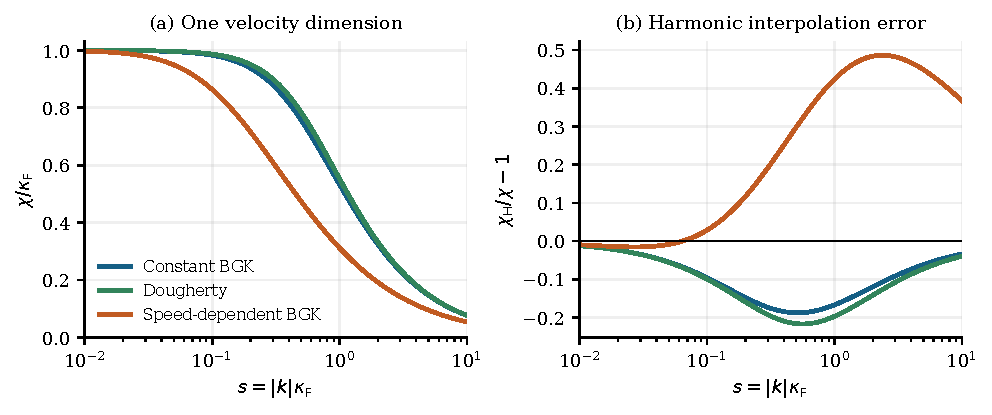
\includegraphics[width=\textwidth]{figures/relaxation_comparison.pdf}
\caption{One-dimensional responses with physical energy flux.
(a) Conductivity matching leaves a substantial difference between collision
models. (b) Signed relative error of the harmonic interpolant
\eqref{eq:harmonic}; positive values mean an overestimate.
Curves use saved quadrature results, with no fitted parameters.}
\label{fig:relaxation}
\end{figure}

A common way to interpolate between the two endpoints is the harmonic
interpolant
\begin{equation}
 \chi_{\rm H}(k)=
 \left(\F^{-1}+\frac{|k|}{\theta_\infty}\right)^{-1}.
 \label{eq:harmonic}
\end{equation}
Figure~\ref{fig:relaxation} shows that this interpolant is too low for
the constant-rate models over the displayed range, but that it crosses
above the speed-dependent BGK response at intermediate $s$.
There is also a simple reason that the interpolant cannot be right near
the origin. Whereas
$\chi/\F=1-Kk^2+o(k^2)$, the interpolant satisfies
\[
 \chi_{\rm H}/\F
      =1-(\F/\theta_\infty)|k|+O(k^2).
\]
In other words, it has the wrong first correction at the origin, and so
it underestimates every model covered by \cref{thm:leading} at
\emph{sufficiently small} nonzero $k$, including the variable-rate
example. The sign reversal that we observe happens at finite wavenumber;
it is not a property of Coulomb-like relaxation at all wavenumbers.

\subsection{Landau transport constants and refinement}

\begin{table}[tb]
\centering
\caption{Landau transport quantities from the degree hierarchy.
All values use \eqref{eq:landauform}. The relatively fast convergence
of $\F$ does not imply equally fast convergence of $K$.}
\label{tab:landauconstants}
\begin{tabular}{rrrrrr}\toprule
$D$ & $\kappa_{\rm F}/\tau$ & $\eta/\tau$ & $C/\tau$ & $X_0/\tau$ & $K/\tau^2$\\\midrule
6 & 3.906250 & 0.965282 & 4.30792 & 0.88314 & 15.67789 \\
8 & 3.950050 & 0.965288 & 5.95775 & 0.81311 & 22.46279 \\
10 & 3.950180 & 0.965291 & 5.93696 & 0.81525 & 22.37857 \\
12 & 3.950196 & 0.965292 & 5.92781 & 0.81526 & 22.34253 \\
16 & 3.950208 & 0.965292 & 5.92911 & 0.81527 & 22.34774 \\
\bottomrule\end{tabular}

\end{table}

Table~\ref{tab:landauconstants} gives
$\F/\tau\simeq3.9502$, $\eta/\tau\simeq0.9653$ and
$K/\tau^2\simeq22.35$. The normalized coefficient is
$c_{\rm L}\simeq1.432$, compared with $c_{\rm D}=0.192$:
a ratio of approximately $7.45$ for two three-dimensional models at
equal conductivity. This compares asymptotic curvatures. It does not
say that the errors of the two models have that ratio at every $k$.

\begin{table}[tb]
\centering
\caption{Landau response refinement and quadratic asymptote.
The difference is the absolute difference of the two normalized
responses, not a rigorous error estimate. The small-$k$ expansion
is deliberately not extrapolated across the entire table.}
\label{tab:landaucurves}
\small
\begin{tabular}{rrrrr}\toprule
$|k|\tau$ & $\chi_{12}/\kappa_{12}$ & $\chi_{16}/\kappa_{16}$ & Difference & $1-K_{16}k^2$\\\midrule
0.005 & 0.999443 & 0.999443 & 1.2e-07 & 0.999441 \\
0.010 & 0.997788 & 0.997788 & 4.2e-07 & 0.997765 \\
0.020 & 0.991405 & 0.991404 & 9.4e-07 & 0.991061 \\
0.050 & 0.954261 & 0.954290 & 2.9e-05 & 0.944131 \\
0.100 & 0.870950 & 0.871115 & 1.7e-04 & 0.776523 \\
0.200 & 0.727113 & 0.727166 & 5.3e-05 & --- \\
0.300 & 0.626028 & 0.627579 & 1.6e-03 & --- \\
0.500 & 0.501588 & 0.502997 & 1.4e-03 & --- \\
1.000 & 0.349755 & 0.350566 & 8.1e-04 & --- \\
\bottomrule\end{tabular}

\end{table}

At $|k|\tau=0.1$, the computed conductivity is $0.8711\F$, a
$12.9\%$ deficit. At the same conductivity-scaled wavenumber
$s\simeq0.395$, the Dougherty deficit is only about $3\%$.
At $|k|\tau=0.3$, the degree-12 to degree-16 difference is approximately
$1.5\times10^{-3}$, so we cannot report six converged digits of the
continuum closure there.
The quadratic asymptote at $|k|\tau=0.1$ is already visibly less
accurate than the computed response. Asymptotic truncation and Galerkin
truncation are different errors.

\begin{figure}[tb]
\centering
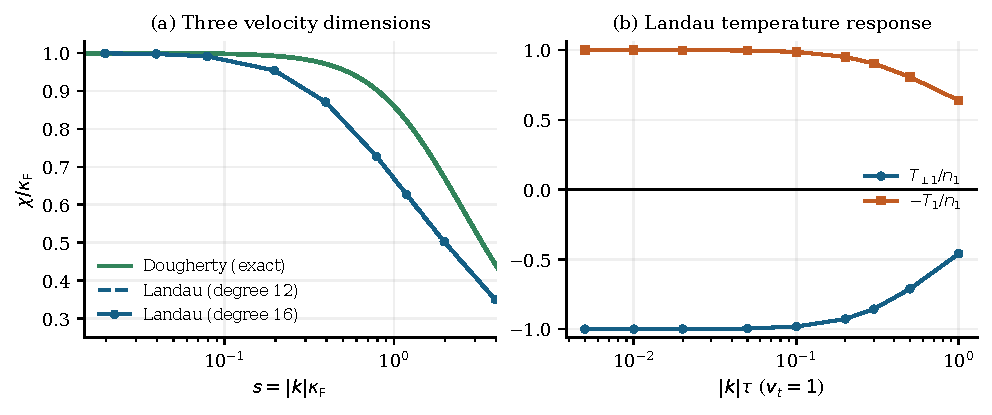
\includegraphics[width=\textwidth]{figures/landau_comparison.pdf}
\caption{(a) Three-dimensional conductivity at matched $s=|k|\F$.
For the Landau refinement curves, the horizontal scale uses the
degree-16 conductivity; the ratios use each degree's own conductivity.
(b) The Landau perpendicular-temperature response remains negative
at all sampled points, consistent with positive heat conduction.
These are finite-degree observations and do not establish an
all-wavenumber theorem.}
\label{fig:landau}
\end{figure}

The positivity criterion gives the \emph{estimated} threshold
$|k|\tau\simeq\sqrt{3/(3.9502\cdot0.9653)}\simeq0.887$.
That number is an estimate. The calculation does not certify it, and
the rigorous statement is still $k^2\F\eta<3$ with the exact
coefficients. The data also support
$-n_1\leq T_{\perp1}\leq0$ over the sampled interval
(\cref{fig:landau}), but they do not prove it outside that interval or
in the continuum. For the potential drive, we leave open an all-$k$
proof of positivity and a proof of $\chi<\F$ for Landau. For the thermal
drive, \cref{cor:th-electronbounds} gives both.

\subsection{An embedded initial-value test}\label{sec:embedded}

Getting the static response right is one thing; using it as a closure in
\eqref{eq:hierarchy} is another, and it has to be tested separately.
To do so, we evolve the one-dimensional
Dougherty model with $\nu=1$, no force, and a single spatial Fourier
mode whose velocity amplitude is
$h(0,v)=\He_2(v)/2$. This means $(n,u,T)(0)=(0,0,1)$ and $q(0)=0$.
The unit amplitude stands for a normalized infinitesimal perturbation;
we do not claim that the unscaled linear distribution is nonnegative
everywhere. Reference trajectories use Hermite degrees $64$ and $128$.
We use matrix-exponential actions, which avoid a time-step
discretization.
We compare three closures: the exact quasi-static coefficient
\eqref{eq:doughertyclosed}, Fourier's coefficient $1/2$, and
\eqref{eq:harmonic} with $\theta_\infty=\sqrt{2/\pi}$.
The closed equations are
\begin{equation}
 \dot n=-iku,\qquad \dot u=-ik(n+T),\qquad
 \dot T=-2iku-2k^2\chi T .
 \label{eq:embedded}
\end{equation}
For $\chi>0$ their resolved quadratic energy
$\mathcal E=(|n|^2+|u|^2+|T|^2/2)/2$ satisfies
$\dot{\mathcal E}=-k^2\chi|T|^2\leq0$.
The kinetic energy $\|h\|_{L^2(M)}^2/2$ also decreases.
The zero spatial mode preserves density, momentum and temperature.
These are checks of linear conservation and dissipation; they do not
test nonlinear realizability.

\begin{figure}[tb]
\centering
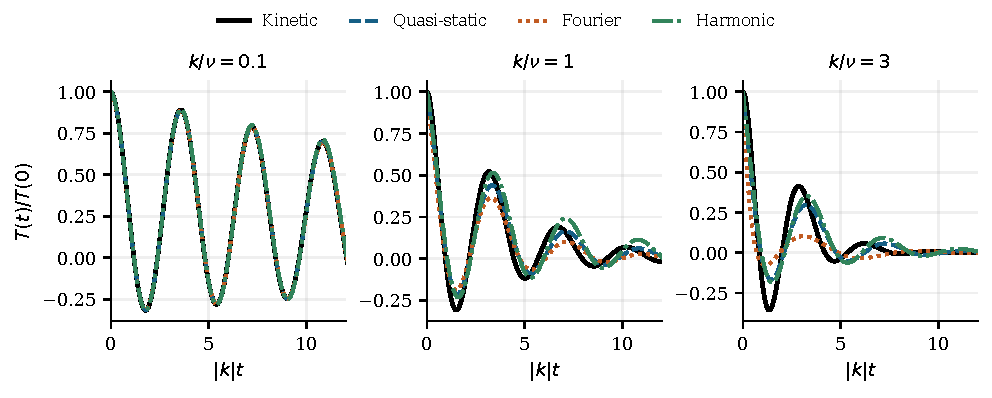
\includegraphics[width=\textwidth]{figures/embedded_rollouts.pdf}
\caption{Freely evolving temperature modes in the one-dimensional
Dougherty model. The exact quasi-static coefficient reduces errors
relative to Fourier in these cases, but does not reproduce the kinetic
transient. Only the first $|k|t=12$ is plotted; errors in
\cref{tab:embedded} use the full interval $0\leq|k|t\leq30$.}
\label{fig:embedded}
\end{figure}

For $U=(n,u,T)$ define
\[
 E_U=\left[
 \frac{\int_0^{30/|k|}\|U_{\rm m}(t)-U_{\rm kin}(t)\|_2^2\dd t}
      {\int_0^{30/|k|}\|U_{\rm kin}(t)\|_2^2\dd t}
 \right]^{1/2}.
\]
We compute this metric with 601 uniform output times and the trapezoidal
rule. It is dimensionless and weights the three moments equally, so it
is not the physical quadratic energy.
Doubling the number of output intervals changes every reported
history error by less than $1.4\times10^{-6}$ in absolute value.
\begin{table}[tb]
\centering
\caption{Embedded history error $E_U$. Kinetic refinement compares
degrees 64 and 128 with the same metric. All candidates satisfy the
linear energy-decay check. Stability does not imply accuracy.}
\label{tab:embedded}
\begin{tabular}{rrrrr}\toprule
$k/\nu$ & Quasi-static & Fourier & Harmonic & Kinetic refinement\\\midrule
0.1 & 0.02028 & 0.02039 & 0.03114 & 9.3e-14 \\
1.0 & 0.23684 & 0.29247 & 0.28443 & 1.8e-14 \\
3.0 & 0.33802 & 0.59308 & 0.35350 & 5.7e-15 \\
\bottomrule\end{tabular}

\end{table}

The quasi-static closure has errors of about $2.0\%$, $23.7\%$ and
$33.8\%$ at $k/\nu=0.1,1,3$, respectively.
These errors are much larger than the kinetic degree-refinement
differences. The reason is already visible at $t=0$: the kinetic heat
flux is zero, whereas the instantaneous law gives
$q_{\rm m}(0)=-ik\chi$. The initial velocity distribution carries
information that the slow-forcing ratio does not specify. We read this
experiment as a negative result about transferring a response formula,
without restriction, to an evolution law. It is not evidence against the
response formula itself. \Cref{sec:memory} identifies the exact law, a
convolution in time whose zero-frequency value is $\chi(k)$, and bounds
the error of replacing it by that value.

\FloatBarrier
\section{Numerical results for the thermal drive and electron collisions}\label{sec:th-numerics}

\subsection{Methods}

All calculations are deterministic; there is no ensemble and no trained
model. We use the polynomial Galerkin basis of \cref{sec:numerics},
$\psi_n(v_x)L_m(v_\perp^2/2)$ with $n+2m\leq D$, and its like-particle
Landau matrices for $D=6,8,10,12,16$. The Lorentz matrix is assembled
from \eqref{eq:th-electron} in spherical coordinates. The factor $|v|^{-1}$
in $U$ combines with the volume element so that the integrand is a
polynomial in $|v|^2/2$ and in the direction of $v$; Gauss--Laguerre,
Gauss--Legendre and periodic quadratures of orders
$\lfloor D/2\rfloor+2$, $D+3$ and $2D+6$ then integrate it exactly in
exact arithmetic. We check every Lorentz matrix for symmetry, a
nonnegative spectrum, the kernel $\{1,|v|^2\}$, the normalization
$\av{|v|^{-1}}=\sqrt{2/\pi}$, and the exact entry
$\av{v_x\Lambda_{ei}v_x}=1/\tau_e$; all hold to about $10^{-14}$.

Because the Lorentz rate behaves like $|v|^{-3}$, the exact solutions are
not smooth at $v=0$ and polynomial approximations converge slowly,
especially at large $Z$. The Galerkin conductivities are lower bounds in
exact arithmetic, since $L_{11}$ and the Schur complement \eqref{eq:th-schur}
are monotone in the trial space. The computed $K_\thr$ is not monotone. We
report differences between degrees as diagnostics; they are not
certified error bars. The bounds \eqref{eq:th-bounds} hold at every computed
point, for every operator and degree, as they must for the Galerkin
problem.

\subsection{Validation against known transport coefficients}

\begin{table}[tb]
\centering
\caption{Electron transport coefficients versus ion charge, with
$\kap$ and $\sigma=L_{11}$ in units of $\tau_e$ and subscripts giving the
degree $D$. The column ``Brag.'' quotes Braginskii's coefficient
$\gamma_0$ \cite{Braginskii1965}. The last three columns give the leading
deficit coefficient in units of $\lambda_e^2$ and in normalized form; $K$ in the
column heads is $K_\thr$.}
\label{tab:th-electron}
\small
\begin{tabular}{rrrrrrrrr}\toprule
$Z$ & $\kappa_6$ & Brag. & $\kappa_{12}$ & $\kappa_{16}$ & $\sigma_{16}$ & $K_{12}/\lambda_e^2$ & $K_{16}/\lambda_e^2$ & $K/\kappa^2$\\\midrule
1 & 3.1616 & 3.1616 & 3.1881 & 3.1967 & 1.9742 & 43.5 & 43.65 & 4.27 \\
2 & 4.8901 & 4.890 & 4.9242 & 4.9294 & 2.3283 & 147 & 147.4 & 6.07 \\
3 & 6.0641 & 6.064 & 6.1124 & 6.1145 & 2.5312 & 287.4 & 288.1 & 7.71 \\
4 & 6.9201 & 6.920 & 6.9934 & 6.9940 & 2.6662 & 452.9 & 453.6 & 9.27 \\
8 & 8.8497 & --- & 9.0643 & 9.0649 & 2.9419 & 1256 & 1255 & 15.27 \\
16 & 10.3336 & --- & 10.7846 & 10.7867 & 3.1350 & 3139 & 3130 & 26.90 \\
64 & 11.8529 & --- & 12.7222 & 12.7249 & 3.3216 & 15563 & 15503 & 95.74 \\
\bottomrule\end{tabular}

\end{table}

\Cref{tab:th-electron} gives the constants. At $D=6$ the odd part of the
basis contains exactly the three Sonine polynomials used by Braginskii,
and we reproduce his heat-conductivity coefficients $3.1616$, $4.890$,
$6.064$ and $6.920$ for $Z=1,2,3,4$ to all quoted digits. At $Z=1$ we
also obtain $\sigma/\tau_e=1.9499$ and $L_{12}/L_{11}=0.7110$, compared
with his $1/0.5129=1.9497$ and $0.711$. These agreements test the relative
normalization of the two collision terms in \eqref{eq:th-electron}, which is
the easiest place to lose a factor of $\sqrt2$. (We did not. We checked.)

As the degree increases, the $Z=1$ values rise to $\kap/\tau_e=3.1967$ and
$\sigma/\tau_e=1.9742$ at $D=16$. They are still increasing slowly, and
they sit just below the values usually quoted from Spitzer and H\"arm
\cite{SpitzerHarm1953}, about $3.20$ and $1.98$. This is the expected
behavior of a lower bound, and the difference between $D=12$ and $D=16$,
about $0.3\%$, is the size of the truncation error we can see.

\begin{table}[tb]
\centering
\caption{Approach to the Lorentz limit $Z\to\infty$, where
$\sigma/\tau_e=32/(3\pi)$ and $\kap/\tau_e=128/(3\pi)$ in closed form.}
\label{tab:th-lorentz}
\small
\begin{tabular}{rrrr}\toprule
$Z$ & $D$ & $\kappa/\tau_e$ & $\sigma/\tau_e$\\\midrule
256 & 12 & 13.3513 & 3.3761 \\
256 & 16 & 13.3536 & 3.3762 \\
4096 & 12 & 13.5641 & 3.3940 \\
4096 & 16 & 13.5662 & 3.3941 \\
$\infty$ & exact & 13.5812 & 3.3953 \\
\bottomrule\end{tabular}

\end{table}

\Cref{tab:th-lorentz} tests the opposite extreme. As $Z\to\infty$ the
Lorentz term dominates and both coefficients are known in closed form. At
$Z=4096$ and $D=16$ we are within $0.11\%$ and $0.04\%$ of them.

\subsection{The deficit coefficient and its dependence on charge}

The last columns of \cref{tab:th-electron} are new. In units of the
collision length, the leading deficit is
$1-\chi_\thr/\kap\simeq43.7\,(k\lambda_e)^2$ for $Z=1$ and
$1.55\times10^4\,(k\lambda_e)^2$ for $Z=64$. Equivalently, the
delocalization length $\sqrt{K_\thr}$ is about $6.6\lambda_e$ at $Z=1$ and
$125\lambda_e$ at $Z=64$. This quantifies the familiar observation that
electron heat conduction becomes nonlocal at $k\lambda_e$ of order
$10^{-2}$ \cite{LMV1983,EpperleinShort1991}.

The normalized coefficient $K_\thr/\kap^2$, which measures the deficit at
matched conductivity, grows from $4.27$ at $Z=1$ to $95.7$ at $Z=64$.
Between $Z=16$ and $Z=64$ the growth is close to linear, with slope about
$1.43$. The reason is visible in \eqref{eq:th-constants}. The conductivity is
set by electron--ion scattering and scales like $1/Z$ in units of
$\tau_{ee}$, whereas $C_\thr$ involves the collision inverse of the isotropic
part of $b_\thr$, which only electron--electron collisions can relax. So
$\sqrt{K_\thr}$ scales like $\sqrt Z\,\lambda_e$, the geometric mean of the
scattering and energy-exchange lengths. \Cref{thm:largeZ} makes this
exact: $K_\thr/\kap^2=(C_\infty/\kap_{\rm L})Z+O(1)$, and the slope is
$1.4305$ (\cref{sec:th-largeZnum}). For
comparison, the like-particle Landau value is $K_\thr/\kap^2=1.69$ for the
thermal drive, so even at $Z=1$ electron--ion scattering makes the
closure about $2.5$ times more nonlocal at matched conductivity.

The degree dependence of $K_\thr$ at fixed $Z$ is the weakest part of the
computation. Between $D=12$ and $D=16$, $K_\thr$ changes by $0.4\%$ at both $Z=1$
and $Z=64$, but between $D=10$ and $D=12$ the change at $Z=1$
is $4.6\%$, so the sequence is not yet monotone and we would not quote
more than two digits.

\begin{figure}[tb]
\centering
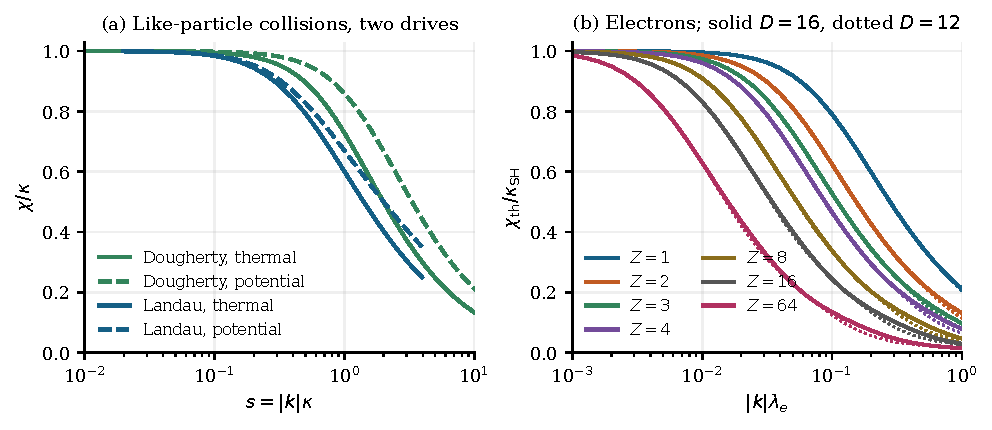
\includegraphics[width=\textwidth]{../electron_heat_flux_extension/figures/responses.pdf}
\caption{(a) Like-particle operators at matched conductivity: the thermal
and potential drives share $\kap$ and differ beyond it. Dougherty curves
are the closed forms; Landau curves are Galerkin solves at $D=16$.
(b) Thermally driven electron response for several ion charges. The gap
between solid and dotted curves is the visible truncation error.}
\label{fig:th-responses}
\end{figure}

\subsection{Response curves and the two drives}

\Cref{fig:th-responses}(b) shows $\chi_\thr/\kap$ against $|k|\lambda_e$. At
$|k|\lambda_e=0.1$ the conductivity is $79\%$ of Spitzer--H\"arm for
$Z=1$ and $34\%$ for $Z=8$. The two degrees agree to plotting accuracy
for $|k|\lambda_e\lesssim0.1$ and separate beyond it, more so at large
$Z$. A polynomial basis cannot resolve the resonant layer at large
$|k|\lambda_e$, and we make no claim there. All curves lie between the
bounds \eqref{eq:th-bounds}.

\begin{table}[tb]
\centering
\caption{Like-particle Landau collisions: the conductivity and the
leading deficit coefficients for the potential and thermal drives.}
\label{tab:th-drives}
\small
\begin{tabular}{rrrrr}\toprule
$D$ & $\kappa/\tau$ & $K_{\rm pot}/\tau^2$ & $K_{\rm th}/\tau^2$ & ratio\\\midrule
6 & 3.906250 & 15.6779 & 19.5555 & 1.2473 \\
8 & 3.950050 & 22.4628 & 26.4761 & 1.1787 \\
10 & 3.950180 & 22.3786 & 26.3892 & 1.1792 \\
12 & 3.950196 & 22.3425 & 26.3532 & 1.1795 \\
16 & 3.950208 & 22.3477 & 26.3584 & 1.1795 \\
\bottomrule\end{tabular}

\end{table}

\Cref{fig:th-responses}(a) and \cref{tab:th-drives} compare the two drives for
like-particle collisions. For Landau the thermal coefficient is
$K_\thr/\tau^2\simeq26.36$, compared with $K_\pot/\tau^2\simeq22.35$, a
ratio of $1.18$. For Dougherty the ratio is $(16/45)/(2/15)=8/3$. In all
of our Landau computations $\chi_\pot\geq\chi_\thr$. We prove this
ordering for BGK, the ellipsoidal-statistical operator and Dougherty, and
show that it is not general (\cref{prop:ce-order}); for Landau it is an
observation.
The thermally driven Landau response is positive and below $\kap$ at
every sampled $k$, which \cref{cor:th-bounds} guarantees for the Galerkin
problem at any $k$ and, by \cref{prop:th-solv}, for the continuum.

\begin{table}[tb]
\centering
\caption{Like-particle Landau collisions: the response matrix
\eqref{eq:th-matrix} at degree $16$, scaled by $|k|$, with the two
quantities of \cref{prop:intermediate}. The refinement column is the
largest change in an entry from degree $12$ to $16$, relative to
$M_{\parallel\parallel}$. The last row is the proved limit of
\cref{cor:th-landaulimit}.}
\label{tab:matrix}
\small
\begin{tabular}{rrrrrrr}\toprule
$|k|\tau$ & $|k|M_{\parallel\parallel}$ & $|k|M_{\parallel\perp}$ & $|k|M_{\perp\perp}$ & $T_{\perp1}/n_1$ & $N_\vartheta/(9n_1)$ & Refinement\\\midrule
0.1 & 2.943 & 2.888 & 3.115 & -0.981 & 0.043 & 2.0e-04 \\
0.3 & 1.487 & 1.273 & 1.807 & -0.856 & 0.223 & 2.4e-03 \\
0.5 & 1.246 & 0.887 & 1.610 & -0.712 & 0.386 & 2.7e-03 \\
1.0 & 1.130 & 0.518 & 1.483 & -0.459 & 0.620 & 4.0e-03 \\
2.0 & 1.134 & 0.278 & 1.408 & -0.245 & 0.778 & 1.3e-02 \\
3.0 & 1.163 & 0.191 & 1.375 & -0.164 & 0.824 & 8.8e-03 \\
5.0 & 1.188 & 0.112 & 1.343 & -0.094 & 0.863 & 3.8e-02 \\
\midrule
$\infty$ & 1.253 & 0 & 1.253 & 0 & 0.889 & --- \\
\bottomrule\end{tabular}

\end{table}

\Cref{tab:matrix} gives the like-particle response matrix itself. The
off-diagonal entry falls from equality with the diagonal at small $k$ to
a tenth of it at $|k|\tau=5$, and the diagonal entries approach
$\sqrt{\pi/2}\simeq1.253$ from opposite sides. Both conditions of
\cref{prop:intermediate} hold at every row, with
$N_\vartheta/(9n_1)$ rising monotonically toward $8/9$. The last rows
are converged to about two digits only; a polynomial basis does not reach
the layer, and this table is evidence, not proof.

\subsection{A check of the Stieltjes structure}\label{sec:th-stcheck}

\Cref{thm:stieltjes} predicts the sign of $\Imag\chi$ at complex $k^2$,
which is easy to test and easy to get wrong. We evaluated the responses at
$56$ points $k^2=re^{i\pi a}$ with $0.01\leq r\leq30$ and
$0.1\leq a\leq0.9$, and at eleven real points, in units $\nu=1$ or
$\tau_{ee}=1$ and with $r$ multiplied by $Z^2$ for electrons. For every case the theorem
covers, $\Imag\chi\leq0$ at every sampled point, $\chi$ decreases and
$k^2\chi$ increases along the real axis. The cases are the closed forms
\eqref{eq:bgkclosed}, \eqref{eq:doughertyclosed} in one dimension and
\eqref{eq:th-dougherty}, continued analytically; the thermally driven
Galerkin responses for Dougherty, Landau and electrons with $Z=1$ and
$8$ at degrees $12$ and $16$; and twenty random finite-dimensional models
of the two quadratic forms. The Dougherty integrals converge only for
$\Real k^2>-\nu^2$, so the closed forms were sampled at the $45$ points
with $\Real k^2>-\nu^2/2$. For the Galerkin problems the theorem holds
exactly, so those runs test the code and not the continuum.

The Dougherty coefficient $K_2=499/2025$ was computed in rational
arithmetic. The upper bound in \eqref{eq:st-pade} then exceeds the exact
$\chi_\thr$ by $0.06\%$ at $k/\nu=0.55$ and by $1\%$ at $k/\nu=1$, where
the lower bound is $6\%$ below.

The potential drive in three dimensions is not covered, and the two
operators behave differently. For Dougherty the closed form and the
Galerkin response satisfy all three sign conditions at every sampled
point; we have no proof. For Landau the Galerkin response has
$\Imag\chi_\pot>0$ at two of the eight points nearest the negative axis,
at each degree. A finite-degree response is a rational function with poles
on the negative axis, so at these degrees some pole of $\chi_\pot$ has a
negative weight. The points differ between the two degrees, and we do not
know what survives in the continuum. On the positive axis $\chi_\pot$ is
monotone at every sampled point.

\subsection{The large-charge limit}\label{sec:th-largeZnum}

The limit problem of \cref{sec:th-largeZ} is radial, so it can be solved
far more accurately than the three-dimensional one, and by different
means. For radial $f$ and $h$ the angular integrals in
\eqref{eq:landauform} can be done in closed form: with $a=|v|$, $b=|v'|$,
\[
 \D_{ee}(f,h)=\frac{3\sqrt\pi}{2\tau_{ee}}\Bigl[\av{A\,f'h'}
  -\frac23\iint M_3M_3'\,f'(a)\,h'(b)\,
     \frac{\min(a,b)}{\max(a,b)^2}\dd v\dd v'\Bigr],
\]
where $A(a)=\tfrac{8\pi}3\int_0^\infty M_3(b)\,b^4\max(a,b)^{-3}\dd b$ is
elementary. We discretize with polynomials in $|v|$, not in $|v|^2$,
orthonormal for the radial Maxwellian weight, of degree up to $64$. This
basis contains $b_\infty$ and $w$ exactly. The kernel has a kink on the
diagonal; the inner integral is split there and evaluated with running
integrals on a composite Gauss--Legendre grid, $320$ panels of ten nodes
on $0\leq|v|\leq16$.

Three checks. The form annihilates $1$ and $|v|^2$ to $3\times10^{-12}$.
Restricted to even polynomials of degree at most $12$ and $16$, its
eigenvalues agree with those of the radial block of the cached
three-dimensional Landau matrices to $2\times10^{-14}$; the two assemblies
share no code. And the quadrature of $\av{w\varphi_0^2}$ reproduces
$\kap_{\rm L}=64\sqrt2/(3\pi)$ to rounding.

The result is
\[
 C_\infty=13.737821,\qquad \frac{C_\infty}{\kap_{\rm L}}=1.430520,\qquad
 \kap_{\rm L}C_\infty=131.9294,
\]
unchanged to ten digits between degrees $32$ and $64$ and between $160$
and $320$ panels. Unlike the constants of \cref{tab:th-electron}, these
digits are converged, although the convergence is observed and not
certified.

\begin{table}[tb]
\centering
\caption{Approach to the large-charge limit of \cref{thm:largeZ} in the
three-dimensional Galerkin computation at degrees $12$ and $16$, in units
$\tau_{ee}=1$. The last row is the limit, computed with the radial
solver.}
\label{tab:th-largeZ}
\small
\begin{tabular}{rrrrrrr}\toprule
$Z$ & $Z\kappa_{12}/\kappa_{\rm L}$ & $Z\kappa_{16}/\kappa_{\rm L}$ & $C_{\thr,12}$ & $C_{\thr,16}$ & $K_{12}/(\kappa^2Z)$ & $K_{16}/(\kappa^2Z)$\\\midrule
1 & 0.2347 & 0.2354 & 9.647 & 9.656 & 4.279 & 4.272 \\
4 & 0.5149 & 0.5150 & 11.449 & 11.465 & 2.315 & 2.318 \\
16 & 0.7941 & 0.7942 & 12.862 & 12.824 & 1.687 & 1.681 \\
64 & 0.9367 & 0.9369 & 13.516 & 13.461 & 1.502 & 1.496 \\
256 & 0.9831 & 0.9832 & 13.721 & 13.666 & 1.453 & 1.447 \\
1024 & 0.9956 & 0.9957 & 13.776 & 13.722 & 1.441 & 1.435 \\
4096 & 0.9987 & 0.9989 & 13.790 & 13.736 & 1.438 & 1.432 \\
\midrule
$\infty$ & \multicolumn{2}{c}{1} & \multicolumn{2}{c}{13.738} & \multicolumn{2}{c}{1.431} \\
\bottomrule\end{tabular}

\end{table}

\Cref{tab:th-largeZ} compares with the three-dimensional computation.
$Z\kap$ increases toward $\kap_{\rm L}$, as the theorem says it must, and
at $Z=4096$ and degree $16$ the three-dimensional values are
$C_\thr=13.736$ and $K_\thr/(\kap^2Z)=1.432$. The remaining differences
are comparable to the change between the two degrees, so this is
agreement within the truncation error of the three-dimensional basis and
no better. Earlier we estimated the slope as $1.43$ from the values at
$Z=16$ and $64$; the approach to the limit is slow in $Z$, as the table
shows, and that estimate was better than it had a right to be.

\begin{figure}[tb]
\centering
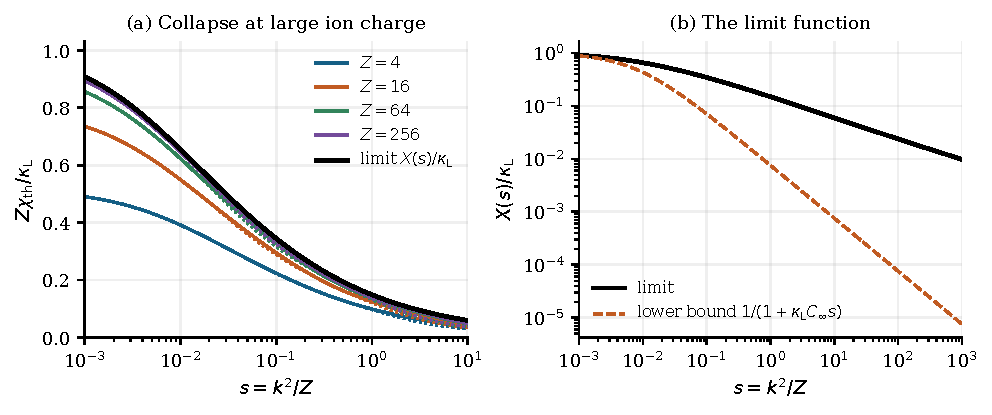
\includegraphics[width=\textwidth]{figures/large_z.pdf}
\caption{(a) The scaled conductivity $Z\chi_\thr/\kap_{\rm L}$ against
$s=k^2/Z$ for several ion charges (three-dimensional Galerkin, degree
$16$ solid and $12$ dotted) and the limit $X(s)/\kap_{\rm L}$ of
\cref{thm:LZ-limit} (radial solver). (b) The limit function and its lower
bound from \eqref{eq:LZ-Xbounds}.}
\label{fig:th-largeZ}
\end{figure}

\Cref{fig:th-largeZ}(a) shows the collapse. At every sampled point with
$s\leq10$ the finite-$Z$ curves lie below the limit, as
\eqref{eq:LZ-chi} requires; the largest ratio is $0.988$, at $Z=256$. At
$s=10^{-2}$ the ratio is $0.60$, $0.84$, $0.95$ and $0.99$ for
$Z=4,16,64,256$, consistent with an error of order $1/Z$. Beyond
$s\approx1$ the two degrees separate and the three-dimensional curves are
not converged.

The limit function departs from its small-$s$ expansion very early
(\cref{fig:th-largeZ}(b)). The ratio $(1-X/\kap_{\rm L})/s$ is $131.9$ at
$s=10^{-6}$ and has already fallen to $91.8$ at $s=10^{-3}$, where the
deficit is $9\%$. Half of the conductivity is gone at $s\approx0.03$,
that is at $k\lambda_e\approx0.13/\sqrt Z$. At large $s$ the local
exponent $\dd\log X/\dd\log s$ is $-0.40$ between $s=1$ and $100$,
$-0.36$ near $10^4$ and $-0.33$ near $10^6$; at $s=10^6$ the value of $X$
still changes by $6\times10^{-4}$ between degrees $48$ and $64$. We do
not extrapolate the exponent.

\subsection{An embedded test: decay of a temperature perturbation}\label{sec:th-embedded}

A static response is not an evolution law until it has been tested as
one. The natural experiment here is the decay of an electron temperature
perturbation, the setting of \cite{EpperleinShort1991}. The kinetic model
is \eqref{eq:th-kinetic} with $p=0$ and with the ambipolar force chosen at
each time so that the current vanishes:
\begin{equation}
 \partial_th=-P\,(ikv_x+\Lambda_Z)\,Ph,\qquad
 P=1-|v_x\rangle\langle v_x| ,\qquad h(0)=\tfrac12(|v|^2-3).
 \label{eq:th-kineticqn}
\end{equation}
The initial condition is a Maxwellian with a temperature perturbation,
$T(0)=1$ and $n=u=q=0$. The density and current remain zero, and
$\|h\|_{L^2(M)}$ is nonincreasing; we verify both numerically. The exact
energy equation is $\tfrac32\dot T=-ikq$, so the closed model is
\begin{equation}
 \tfrac32\dot T=-k^2\chi\,T .
 \label{eq:th-closed}
\end{equation}
We compare three choices of $\chi$: the quasi-static thermal response
$\chi_\thr(k)$, the local value $\kap$, and the value that makes
\eqref{eq:th-closed} decay at the rate of the least-damped kinetic mode
carrying temperature. Time is advanced with a matrix exponential, so
there is no time-step error. The error is the relative $L^2$ error of
$T(t)$ over six quasi-static decay times, computed with $601$ samples and
the trapezoidal rule. The reference uses $D=16$, and the column
``Refinement'' applies the same metric to the difference between the
$D=12$ and $D=16$ kinetic solutions.

\begin{table}[tb]
\centering
\caption{Embedded history error of the closed temperature equation
\eqref{eq:th-closed} for three conductivities. Errors smaller than the
refinement column are not resolved.}
\label{tab:th-embedded}
\small
\begin{tabular}{rrrrrrrr}\toprule
$Z$ & $|k|\lambda_e$ & $t_{\rm decay}/\tau_e$ & $\chi_{\rm th}/\kappa$ & Quasi-static & Spitzer--H\"arm & Least-damped & Refinement\\\midrule
1 & 0.01 & 4713 & 0.9957 & 0.0003 & 0.0031 & 0.0004 & 1.9e-03 \\
1 & 0.03 & 540.1 & 0.9654 & 0.0021 & 0.0248 & 0.0030 & 2.0e-03 \\
1 & 0.1 & 59.34 & 0.7907 & 0.0103 & 0.1561 & 0.0144 & 4.2e-03 \\
1 & 0.3 & 10.87 & 0.4798 & 0.0202 & 0.4230 & 0.0202 & 5.2e-04 \\
8 & 0.01 & 1818 & 0.9102 & 0.0015 & 0.0649 & 0.0020 & 8.9e-05 \\
8 & 0.03 & 274.8 & 0.6691 & 0.0038 & 0.2556 & 0.0051 & 2.9e-04 \\
8 & 0.1 & 49.01 & 0.3376 & 0.0401 & 0.5662 & 0.0693 & 6.7e-03 \\
8 & 0.3 & 12.4 & 0.1483 & 0.1141 & 0.7716 & 0.2220 & 5.3e-02 \\
\bottomrule\end{tabular}

\end{table}

\begin{figure}[tb]
\centering
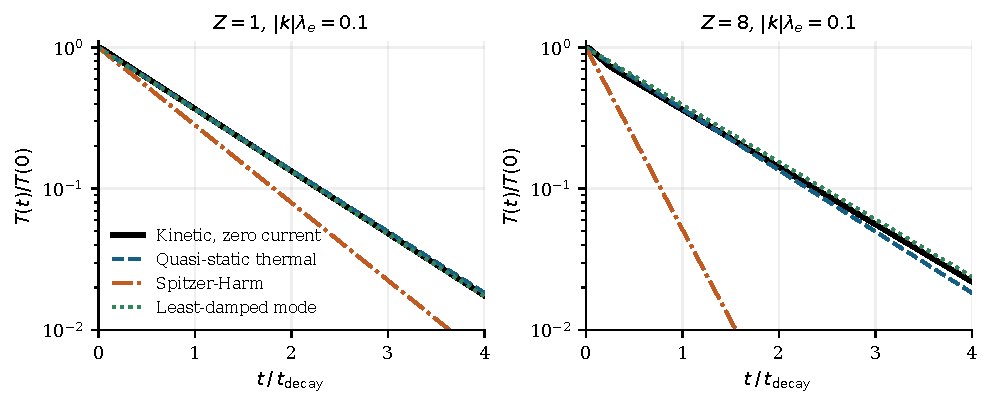
\includegraphics[width=\textwidth]{../electron_heat_flux_extension/figures/embedded_decay.pdf}
\caption{Decay of a temperature perturbation at $|k|\lambda_e=0.1$ in
the quasi-neutral kinetic model and in the closed equation
\eqref{eq:th-closed}.}
\label{fig:th-embedded}
\end{figure}

\Cref{tab:th-embedded} and \cref{fig:th-embedded} give the results. For $Z=1$
the quasi-static closure has errors of $1\%$ at $|k|\lambda_e=0.1$ and
$2\%$ at $0.3$, where the conductivity has dropped to $48\%$ of its local
value and Spitzer--H\"arm conduction is off by $42\%$. For $Z=8$ the
errors are $0.4\%$ at $|k|\lambda_e=0.03$ and $4\%$ at $0.1$. The entry
at $Z=8$, $|k|\lambda_e=0.3$ has a refinement difference of $5\%$, so its
$11\%$ model error is only partly resolved, and we do not interpret it.
At the two smallest wavenumbers for $Z=1$ the model errors are below the
refinement difference, which there reflects the $0.3\%$ change in $\kap$
between degrees.

This is a much better outcome than the embedded test of \cref{sec:embedded}, where the exact quasi-static closure had errors of $24\%$ and
$34\%$. Why? The difference is the time scale, and \cref{sec:memory} turns
this into a bound. There, the temperature
was coupled to sound waves with frequencies comparable to the collision
rate. Here, quasi-neutrality removes the acoustic dynamics and the
temperature decays over $10$ to several thousand collision times
(\cref{tab:th-embedded}), so a zero-frequency response is the appropriate
one. The quasi-static closure is also at least as accurate as the
least-damped-mode closure, which matches the late-time rate exactly but
not the initial layer.

\FloatBarrier
\section{A frequency-dependent closure and the error of the quasi-static one}\label{sec:memory}

The quasi-static coefficient is the value at zero frequency of a
frequency-dependent response. In this section we write that response as a
resolvent of the kinetic operator compressed to the unresolved subspace,
show that it is positive real, and bound the error that the quasi-static
closure makes in an initial-value problem by the variation of the response
over the frequencies that the closed model excites. The bound is small in
the quasi-neutral test of \cref{sec:th-embedded} and of order one in the
sound-wave test of \cref{sec:embedded}.

\subsection{Setting}

Let $d=1$ or $3$. Let $\mathcal Y$ be the orthogonal complement of
$\operatorname{span}\{1,v_x,|v|^2\}$ in complex $L^2(M_d)$, restricted to
axisymmetric functions when $d=3$, and let $\Pi$ be the orthogonal
projection onto $\mathcal Y$. We write $\av{fg}$ for the bilinear pairing,
$(f,g)=\av{\bar fg}$ for the Hermitian one, and $\norm f^2=(f,f)$. In this
section $s$ is a Laplace variable. It is related to the frequency of
\cref{sec:setting} by $s=-i\omega$, so that $\Real s=\Imag\omega$ and
$\widehat h(s)=\int_0^\infty e^{-st}h(t)\dd t$; it is not the scaled
wavenumber of \eqref{eq:units}. Define the compressed operator, the two
unresolved flux functions, and the kernel
\begin{equation}
 B_k=\Pi\,\A_k\,\Pi\big|_{\mathcal Y},\qquad
 Q=Q_d,\qquad \varsigma=v_x^2-\tfrac13|v|^2=-\tfrac13\vartheta\quad(d=3),
 \label{eq:mem-B}
\end{equation}
\begin{equation}
 \chi(k,s)=\av{Q\,(B_k+s)^{-1}Q},\qquad
 \mathsf K(k,s)=
 \begin{pmatrix}
 \av{Q\,(B_k+s)^{-1}Q}&\av{Q\,(B_k+s)^{-1}\varsigma}\\[2pt]
 \av{\varsigma\,(B_k+s)^{-1}Q}&\av{\varsigma\,(B_k+s)^{-1}\varsigma}
 \end{pmatrix}.
 \label{eq:mem-chi}
\end{equation}
Both $Q$ and $\varsigma$ lie in $\mathcal Y$, and $\pi=\av{\varsigma h}$ is
the stress of \eqref{eq:hierarchy}. The projections that produce them are
\begin{equation}
 \Pi(v_x)=0,\qquad \Pi(v_x^2)=\varsigma\ \ (d=3),\quad \Pi(v^2)=0\ \ (d=1),
 \qquad \Pi(v_x\zeta_d)=\tfrac2d\,Q_d .
 \label{eq:mem-proj}
\end{equation}
The last one follows from $v_x\zeta_d=\tfrac2d(Q_d+v_x)$.

\begin{assumption}[Evolution]\label[assumption]{ass:mem-evolution}
One of the following holds.
\begin{enumerate}[label=(\alph*)]
\item \emph{Galerkin.} $L^2(M_d)$ is replaced by a finite-dimensional space
of polynomials that contains every polynomial of degree at most three and
is invariant under reflection in $v_x$ and under complex conjugation, and
$\A_k$ is the Galerkin compression of $ikv_x+\Lambda$ to it.
\item \emph{Continuum.} $-\A_k$ generates a contraction semigroup on
$L^2(M_d)$; the polynomials of degree at most three lie in the domains of
$\A_k$ and $\A_k^*$, on which these operators act as $ikv_x+\Lambda$ and
$-ikv_x+\Lambda$; and $\A_k^*=\overline{\A_k}$, the complex conjugate
operator.
\end{enumerate}
\end{assumption}

Alternative~(b) holds for constant-frequency BGK and for the Dougherty
operator, which are finite-rank perturbations of $ikv_x+\nu$ and of
$ikv_x+\nu N$. This is standard, and we do not write out the
generation argument. We do not verify it for the Landau operator. For
$\Lambda_Z$ it fails as stated, because
$\Lambda_{ei}v_x=\nu_{ei}(v)v_x$ grows like $|v|^{-2}$ at the origin and is
not in $L^2(M)$; a form version of the reduction below would be needed,
and we do not supply one. For the Landau and electron operators the
results of this section are therefore statements about the Galerkin
truncations of \cref{sec:numerics,sec:th-numerics}.

Under either alternative $B_k$ is accretive,
\begin{equation}
 \Real\,(y,B_ky)=\Real\,(y,\A_ky)\ \geq0,\qquad
 \Real\,(y,B_ky)=\D[\Real y]+\D[\Imag y]\ \text{ in case (a)},
 \label{eq:mem-accretive}
\end{equation}
and $B_k+s$ is boundedly invertible on $\mathcal Y$ for $\Real s>0$, with
$\norm{(B_k+s)^{-1}}\leq1/\Real s$. In case~(a) this is immediate. In
case~(b), $1-\Pi$ has finite rank with range in the domains of $\A_k$ and
$\A_k^*$, so $\A_k-\Pi\A_k\Pi$ is bounded; a bounded perturbation of a
generator is a generator, and an accretive generator generates a
contraction semigroup. We write $e^{-tB_k}$ for this semigroup on
$\mathcal Y$.

\subsection{The exact closure for data in the retained space}

\begin{theorem}[Memory form of the closure]\label{thm:mem-closure}
Assume \cref{ass:mem-evolution}. Let $h$ solve
\begin{equation}
 \partial_th+\A_kh=p(t)\,\zeta_d+a(t)\,v_x,\qquad
 h(0)\in\operatorname{span}\{1,v_x,|v|^2\},
 \label{eq:mem-kinetic}
\end{equation}
with bounded $p$ and $a$. Then for $\Real s>0$:
\begin{enumerate}[label=(\roman*)]
\item If $d=1$ and $\Lambda$ conserves mass, momentum and energy,
\begin{equation}
 \widehat q(s)=-ik\,\chi(k,s)\,\widehat T(s).
 \label{eq:mem-1d}
\end{equation}
\item If $d=3$ and $\Lambda$ conserves mass, momentum and energy,
\begin{equation}
 \begin{pmatrix}\widehat q\\ \widehat\pi\end{pmatrix}
 =-ik\,\mathsf K(k,s)
 \begin{pmatrix}\widehat T\\ \widehat u\end{pmatrix}.
 \label{eq:mem-3d}
\end{equation}
\item If $d=3$, $\Lambda$ satisfies \eqref{eq:th-kernel}, $\av{v_xh(0)}=0$,
and the force $a(t)$ is the one that keeps $u(t)=0$ for all $t$, which is
the quasi-neutral model \eqref{eq:th-kineticqn} with a heating source
added, then $\widehat q=-ik\,\chi(k,s)\,\widehat T$ with the same
$\chi=\mathsf K_{qq}$, and
\begin{equation}
 \widehat T(s)=\frac{T(0)+\tfrac23\widehat p(s)}
                    {s+\tfrac23k^2\chi(k,s)} .
 \label{eq:mem-T}
\end{equation}
\end{enumerate}
In each case the unresolved part of the solution is
$\Pi\widehat h=-ik\,(B_k+s)^{-1}(\widehat T\,Q+\widehat u\,\varsigma)$,
with the term in $\varsigma$ absent when $d=1$ or $u=0$. In the time
domain, with $K_k(t)=\av{Q\,e^{-tB_k}Q}$,
\begin{equation}
 q(t)=-ik\int_0^tK_k(t-t')\,T(t')\dd t'
 \label{eq:mem-time}
\end{equation}
in cases (i) and (iii), and the same with the matrix kernel
$\av{b_i\,e^{-tB_k}b_j}$, $b=(Q,\varsigma)$, in case (ii).
\end{theorem}

\begin{proof}
The solution grows at most linearly in $L^2(M_d)$, so its transform exists
for $\Real s>0$ and satisfies
$s\widehat h-h(0)+\A_k\widehat h=\widehat p\,\zeta_d+\widehat a\,v_x$.
Apply $\Pi$. It annihilates $h(0)$, $\zeta_d$ and $v_x$, so
$s\,\Pi\widehat h+\Pi\A_k\widehat h=0$: neither the data nor the sources,
and in particular not the force, enter the unresolved equation. Write
$\widehat h=(1-\Pi)\widehat h+y$ with $y=\Pi\widehat h$. Since
$\norm{\zeta_d}^2=2/d$,
\[
 (1-\Pi)\widehat h=\widehat n+\widehat u\,v_x+\tfrac d2\,\widehat T\,\zeta_d .
\]
In cases (i) and (ii) $\Lambda$ annihilates this function. In case (iii)
it need not annihilate $v_x$, but $\widehat u=0$. In all cases, therefore,
$\A_k(1-\Pi)\widehat h=ikv_x(1-\Pi)\widehat h$, and \eqref{eq:mem-proj}
gives
\[
 \Pi\A_k(1-\Pi)\widehat h=ik\bigl(\widehat u\,\varsigma+\widehat T\,Q\bigr),
\]
with $\varsigma$ replaced by zero when $d=1$. Hence
$(B_k+s)y=-ik(\widehat T\,Q+\widehat u\,\varsigma)$, and $B_k+s$ is
invertible. Because $Q$ and $\varsigma$ lie in $\mathcal Y$,
$\widehat q=\av{Qy}$ and $\widehat\pi=\av{\varsigma y}$. This proves
\eqref{eq:mem-1d} and \eqref{eq:mem-3d} and the first statement of (iii).
In case (iii) pair \eqref{eq:mem-kinetic} with the collision invariant
$\tfrac12(|v|^2-3)=\tfrac32\zeta$ and use
$\tfrac12v_x(|v|^2-3)=Q+v_x$ and $u=0$:
$\tfrac32(s\widehat T-T(0))=-ik\widehat q+\widehat p$. Inserting
$\widehat q=-ik\chi\widehat T$ gives \eqref{eq:mem-T}. Finally
$(B_k+s)^{-1}=\int_0^\infty e^{-st}e^{-tB_k}\dd t$ for $\Real s>0$, and a
product of transforms is the transform of a convolution, which is
\eqref{eq:mem-time}.
\end{proof}

Three remarks. First, \cref{sec:setting} says that the ratio
$\widehat q/\widehat T$ is tied to its input. The theorem makes this
precise in one dimension: the ratio is the same function
$-ik\chi(k,s)$ for every force $a(t)$ and for every initial condition in
$\operatorname{span}\{1,v,v^2\}$. What changes it is initial data, or a
source, with a component $h_\perp$ in $\mathcal Y$, which adds
$\av{Q\,(B_k+s)^{-1}h_\perp}$ to $\widehat q$. Second, the initial
condition of \cref{sec:embedded} lies in the retained space, so
\eqref{eq:mem-time} applies to it and gives $q(0)=0$: the mismatch
$q_{\rm m}(0)=-ik\chi$ noted there is the difference between a convolution
and its instantaneous replacement. Third, for constant-frequency BGK,
$\Lambda=\nu(1-\Pi_H)$ with $\Pi_H$ the projection on the collision
invariants, so $\Lambda=\nu$ on $\mathcal Y$ and
$B_k+s=ik\,\Pi v\Pi+(\nu+s)$: the kernel depends on $s$ and $\nu$ only
through $s+\nu$. This is the statement after \eqref{eq:bgkfrequency} that
the collisional response is a collisionless one at a shifted phase
velocity. Comparing \eqref{eq:mem-1d} with \eqref{eq:bgkfrequency}, which
is derived in \cref{app:bgk} for the same forced problem,
\begin{equation}
 -ik\,\chi(k,-i\omega)=\sgn(k)\,\Phi\Bigl(\frac{\omega+i\nu}{|k|}\Bigr),
 \qquad \Imag\omega>0,
 \label{eq:mem-bgk}
\end{equation}
since two exact expressions for $\widehat q/\widehat T$ must agree
wherever $\widehat T\ne0$, and both sides are analytic.

\subsection{The static value, and one kernel for two drives}

\begin{proposition}[Zero frequency]\label[proposition]{prop:mem-static}
Assume \cref{ass:mem-evolution}, and suppose that $B_k$ is invertible on
$\mathcal Y$ and that the stationary solutions used below exist. In
case~(a) both hold for every $k\ne0$ when the kernel of $\Lambda$
satisfies \eqref{eq:th-kernel}.
\begin{enumerate}[label=(\roman*)]
\item For $d=1$, $\chi(k,0)$ is the quasi-static coefficient $\chi(k)$ of
\eqref{eq:chi}.
\item For $d=3$ and $\Lambda$ satisfying \eqref{eq:th-kernel},
$\mathsf K_{qq}(k,0)=\chi_\thr(k)$.
\item For $d=3$ and $\Lambda$ conserving momentum,
\begin{equation}
 \chi_\pot(k)=\frac{\mathsf K_{qq}(k,0)}{1-ik\,\mathsf K_{q\pi}(k,0)},
 \label{eq:mem-chipot}
\end{equation}
where $\mathsf K_{q\pi}$ is the off-diagonal entry of $\mathsf K$.
\end{enumerate}
For real $s\geq0$ the matrix $\mathsf K(k,s)$ is symmetric, its diagonal
entries are real, even in $k$ and nonnegative (positive in case~(a)), and
$\mathsf K_{q\pi}$ is purely imaginary and odd in $k$.
\end{proposition}

\begin{proof}
In case~(a), if $B_ky=0$ then $\D[\Real y]+\D[\Imag y]=0$ by
\eqref{eq:mem-accretive}, so $y\in\N\cap\mathcal Y=\{0\}$; the same
argument with \eqref{eq:th-kernel} shows that $\A_kg=0$ forces
$g\in\N$, so $\Lambda g=0$ and then $v_xg=0$, hence $g=0$, so the stationary
problems are solvable.

Let $g=\A_k^{-1}\zeta$ be the thermal solution \eqref{eq:th-g}. By
\eqref{eq:th-identities}, $\av{v_xg}=0$ and $\av{Qg}=1/(ik)$. Apply $\Pi$
to $\A_kg=\zeta$ and repeat the computation in the proof of
\cref{thm:mem-closure} with $s=0$, $\widehat u=0$ and
$\widehat T=T_\thr$: $\Pi g=-ikT_\thr B_k^{-1}Q$. Pairing with $Q$ gives
$1/(ik)=-ikT_\thr\mathsf K_{qq}(k,0)$, that is
$\mathsf K_{qq}(k,0)=1/(k^2T_\thr)=\chi_\thr$. This is (ii).

Let now $g=\A_k^{-1}1$ with $\Lambda$ conserving momentum. By
\eqref{eq:stationarymom}, $\av{v_xg}=1/(ik)$ and $\av{Qg}=i/k$. The same
computation, now with $\widehat u=1/(ik)$ and $\widehat T=T_1$, gives
$\Pi g=-B_k^{-1}(\varsigma+ikT_1Q)$, and pairing with $Q$,
\[
 \frac ik=-\mathsf K_{q\pi}-ikT_1\mathsf K_{qq},
 \qquad
 T_1=-\frac{1-ik\,\mathsf K_{q\pi}}{k^2\,\mathsf K_{qq}} ,
\]
which with $\chi_\pot=-1/(k^2T_1)$ is \eqref{eq:mem-chipot}. For $d=1$
there is no $\varsigma$, and the same lines give (i).

Symmetry of $\mathsf K$ follows from $\av{f\,B_kg}=\av{g\,B_kf}$. Let
$\mathcal R$ be reflection in $v_x$. Then
$\overline{B_k}=B_{-k}=\mathcal RB_k\mathcal R$, $\mathcal RQ=-Q$ and
$\mathcal R\varsigma=\varsigma$. Hence
$\overline{\mathsf K_{ij}(k,s)}=\mathsf K_{ij}(-k,\bar s)
 =\epsilon_i\epsilon_j\mathsf K_{ij}(k,\bar s)$ with
$\epsilon_q=-1$, $\epsilon_\pi=1$. At real $s$ the diagonal entries are
real and even in $k$ and the off-diagonal one is imaginary and odd.
The sign is \cref{prop:mem-positive} below; at $s=0$ the identity
\eqref{eq:mem-positive} still holds because $B_k$ is invertible.
\end{proof}

So $\chi_\thr$ is a diagonal entry of the static kernel, and $\chi_\pot$
is not. A potential drive sets up a flow together with the temperature
perturbation, with $\widehat u/\widehat T\to(ikT_1)^{-1}$ as
$\omega\to0$, and by \eqref{eq:mem-3d} the heat flux responds to the
velocity gradient through $\mathsf K_{q\pi}$. The ratio
$\widehat q/\widehat T$ then mixes two entries of $\mathsf K$. This is
the obstruction of \cref{sec:3d,prop:th-matrix} seen from the unresolved
side: \cref{prop:mem-positive} controls the quadratic form of
$\mathsf K$, and it does not control the sign of
$1-ik\mathsf K_{q\pi}$. A closure for a three-dimensional
momentum-conserving plasma with flow needs the three independent entries of $\mathsf K$, as functions of $k$ and
$s$. In one dimension, and under the zero-current constraint, a single
scalar suffices.

\subsection{Positivity and dissipation}

\begin{proposition}[Positive-real kernel]\label[proposition]{prop:mem-positive}
Assume \cref{ass:mem-evolution}. For $\Real s>0$ and $c\in\mathbb C^2$,
\begin{equation}
 \Real\sum_{i,j}\bar c_i\,\mathsf K_{ij}(k,s)\,c_j
 =\Real s\,\norm y^2+\Real\,(y,B_ky)\ \geq\ \Real s\,\norm y^2,
 \qquad y=(B_k+s)^{-1}(c_1Q+c_2\varsigma).
 \label{eq:mem-positive}
\end{equation}
In particular $\Real\chi(k,s)>0$ for $\Real s>0$, and the Hermitian part
of $\mathsf K(k,s)$ is positive definite. In case~(a) the right side is
$\Real s\,\norm y^2+\D[\Real y]+\D[\Imag y]$, the identity extends to
$\Real s=0$, and $\Real\chi(k,-i\omega)>0$ for every real $\omega$.
\end{proposition}

\begin{proof}
Let $b=c_1Q+c_2\varsigma$. The functions $Q$ and $\varsigma$ are real, so
$\sum\bar c_i\mathsf K_{ij}c_j=\av{\bar b\,y}=(b,y)=((B_k+s)y,y)$, whose
real part is $\Real s\norm y^2+\Real(y,B_ky)$. This is the energy identity
\eqref{eq:st-key} with the frequency in place of the wavenumber. If the
left side vanishes with $\Real s>0$ then $y=0$ and $b=0$. In case~(a),
$B_k-i\omega$ is invertible because a vector in its kernel has
$\D[\Real y]+\D[\Imag y]=0$, lies in $\N\cap\mathcal Y$ and vanishes; and
if $\D[\Real y]+\D[\Imag y]=0$ for $y=(B_k-i\omega)^{-1}b$, the same
argument gives $y=0$.
\end{proof}

\begin{corollary}[Positive type and energy]\label[corollary]{cor:mem-energy}
Assume \cref{ass:mem-evolution}. The kernel $K_k$ is real, even in $k$,
bounded by $\norm Q^2$, and of positive type: for $\tau>0$ and
$T\in L^2(0,\tau)$, with
$Y(t)=\int_0^te^{-(t-t')B_k}Q\,T(t')\dd t'$,
\begin{equation}
 \Real\int_0^\tau\overline{T(t)}\int_0^tK_k(t-t')T(t')\dd t'\dd t
 =\tfrac12\norm{Y(\tau)}^2+\int_0^\tau\Real\,(Y,B_kY)\dd t\ \geq0 .
 \label{eq:mem-postype}
\end{equation}
Consequently the exactly closed equations, \eqref{eq:hierarchy} with $a=0$
and \eqref{eq:mem-time}, satisfy
$\mathcal E(\tau)\leq\mathcal E(0)$ for the resolved energy
$\mathcal E=\tfrac12(|n|^2+|u|^2+\tfrac d2|T|^2)$, and
$\mathcal E+\tfrac12k^2\norm Y^2$ is nonincreasing. The same holds for the
matrix kernel in case (ii) of \cref{thm:mem-closure}, with
$Y$ driven by $Q\,T+\varsigma\,u$, and for $\mathcal E=\tfrac34|T|^2$ in
case (iii).
\end{corollary}

\begin{proof}
Reality and evenness follow from
$\overline{B_k}=\mathcal RB_k\mathcal R$ and $\mathcal RQ=-Q$, as in the
proof of \cref{prop:mem-static}, and the bound from contractivity. The
function $Y$ solves $\dot Y=-B_kY+Q\,T$, $Y(0)=0$, and
$\av{QY}=K_k*T$. Therefore
\[
 \tfrac12\tfrac{\dd}{\dd t}\norm Y^2
 =-\Real\,(Y,B_kY)+\Real\bigl(\overline{\av{QY}}\,T\bigr)
 =-\Real\,(Y,B_kY)+\Real\bigl(\overline T\,(K_k*T)\bigr),
\]
and integration gives \eqref{eq:mem-postype}. For the energy, multiply the
three equations of \eqref{eq:hierarchy} by $\bar n$, $\bar u$ and
$\bar T$ and take real parts. The terms $-ik(\bar nu+\bar un)$ and
$-ik(\bar uT+\bar Tu)$ are imaginary, and what remains is
\[
 \dot{\mathcal E}=\Real\bigl(-ik\,\bar u\,\pi-ik\,\bar T\,q\bigr)
 =-k^2\,\Real\bigl(\overline T\,(K_k*T)\bigr)
\]
when $\pi=0$, and the analogous quadratic form of the matrix kernel
otherwise. Since $\Pi h=-ikY$, the conserved-or-decreasing quantity
$\mathcal E+\tfrac12k^2\norm Y^2$ is the kinetic energy
$\tfrac12\norm h^2$.
\end{proof}

The energy inequality is a statement about the exact kernel. The
quasi-static model replaces $K_k$ by $\chi(k,0)\,\delta(t)$; it is also
dissipative, but it is a different equation, and we now estimate the
difference.

\subsection{The error of the quasi-static closure}

Fix $k\ne0$ and a number $\chi_0>0$; the case of interest is
$\chi_0=\chi(k,0)$, but the next theorem does not use this. For $d=1$ let
$U=(n,u,T)$ be the moments of the kinetic solution of
\eqref{eq:mem-kinetic} with $p=a=0$, and let $U_{\rm c}$ solve the closed
equations \eqref{eq:embedded} with $\chi=\chi_0$ and the same initial
values:
\[
 \dot U_{\rm c}=-M_0U_{\rm c},\qquad
 M_0=\begin{pmatrix}0&ik&0\\ ik&0&ik\\ 0&2ik&2k^2\chi_0\end{pmatrix},
 \qquad e_T=(0,0,1)^{\mathsf T}.
\]
For $\Real s\geq0$ put
\begin{equation}
 r(s)=(s+M_0)^{-1}e_T,\qquad
 \mu_U(s)=2k^2\,|\chi(k,s)-\chi_0|\,\|r(s)\|_2,\qquad
 \mu_T(s)=2k^2\,|\chi(k,s)-\chi_0|\,|e_T\cdot r(s)| ,
 \label{eq:mem-mu}
\end{equation}
and
\[
 \eta_U=\sup_{\Real s>0}\mu_U(s),\qquad
 \eta_T=\sup_{\Real s>0}\mu_T(s)\ \leq\eta_U ,
\]
which may be infinite. The matrix $s+M_0$ is invertible for
$\Real s\geq0$: if $M_0x=\lambda x$, the weighted energy gives
$\Real\lambda\,(|x_1|^2+|x_2|^2+\tfrac12|x_3|^2)=k^2\chi_0|x_3|^2$, and
$\Real\lambda=0$ forces $x_3=0$, then $x_2=0$ and $x_1=0$ from the third
and second rows. The vector $r(-i\omega)$ is the response of the closed
model to a temperature source at frequency $\omega$. Norms without a
subscript are those of $L^2(0,\infty)$ in time, with the Euclidean norm
for vectors.

\begin{theorem}[Transfer bound]\label{thm:mem-transfer}
Assume \cref{ass:mem-evolution}, $d=1$, a conserving $\Lambda$, and
$h(0)\in\operatorname{span}\{1,v,v^2\}$. Then:
\begin{enumerate}[label=(\roman*)]
\item $\norm{U-U_{\rm c}}\leq\eta_U\,\norm T\leq\eta_U\,\norm U$.
\item Suppose in addition that $\chi(k,\cdot)$ extends to a bounded
continuous function on $\Real s\geq0$ and that $\eta_T<1$. Then
\begin{equation}
 \norm{U-U_{\rm c}}\leq\frac{W}{1-\eta_T},\qquad
 W^2=\frac1{2\pi}\int_{-\infty}^\infty
 \mu_U(-i\omega)^2\,|\widehat T_{\rm c}(-i\omega)|^2\dd\omega ,
 \label{eq:mem-W}
\end{equation}
where $\widehat T_{\rm c}(s)=e_T\cdot(s+M_0)^{-1}U(0)$. Under the same
continuity hypothesis $\eta_U$ and $\eta_T$ are the suprema of
$\mu_U$ and $\mu_T$ over the imaginary axis.
\end{enumerate}
\end{theorem}

\begin{proof}
The moments $U$ are bounded, so their transforms exist for $\Real s>0$.
By \eqref{eq:hierarchy} and \eqref{eq:mem-1d},
$(s+M(s))\widehat U=U(0)$, where $M(s)$ is $M_0$ with $\chi_0$ replaced by
$\chi(k,s)$, and $(s+M_0)\widehat U_{\rm c}=U(0)$. Subtracting,
\begin{equation}
 \widehat U-\widehat U_{\rm c}
 =-2k^2\bigl(\chi(k,s)-\chi_0\bigr)\,\widehat T(s)\,r(s) .
 \label{eq:mem-diff}
\end{equation}
Fix $\varepsilon>0$. Plancherel's theorem on the line
$\Real s=\varepsilon$ and \eqref{eq:mem-diff} give
\[
 \int_0^\infty e^{-2\varepsilon t}\|U-U_{\rm c}\|_2^2\dd t
 =\frac1{2\pi}\int\|(\widehat U-\widehat U_{\rm c})(\varepsilon-i\omega)\|_2^2\dd\omega
 \leq\eta_U^2\int_0^\infty e^{-2\varepsilon t}|T|^2\dd t
 \leq\eta_U^2\norm T^2 .
\]
Let $\varepsilon\downarrow0$ and use monotone convergence. This is (i);
no boundary values of $\chi$ are involved.

For (ii), take the third component of \eqref{eq:mem-diff}:
$\widehat T\,[1+2k^2(\chi-\chi_0)\,e_T\cdot r]=\widehat T_{\rm c}$, so
$|\widehat T|\leq|\widehat T_{\rm c}|/(1-\eta_T)$ for $\Real s>0$.
Insert this in \eqref{eq:mem-diff} and apply Plancherel on
$\Real s=\varepsilon$ as before:
\[
 \int_0^\infty e^{-2\varepsilon t}\|U-U_{\rm c}\|_2^2\dd t
 \leq\frac1{(1-\eta_T)^2}\,\frac1{2\pi}\int
 \mu_U(\varepsilon-i\omega)^2\,|\widehat T_{\rm c}(\varepsilon-i\omega)|^2\dd\omega .
\]
The rational function $\widehat T_{\rm c}$ has no poles in
$\Real s\geq0$ and decays like $1/|s|$, so
$|\widehat T_{\rm c}(\varepsilon-i\omega)|^2\leq C/(1+\omega^2)$ for
$0\leq\varepsilon\leq1$; $\mu_U$ is bounded and continuous on the closed
half-plane. Dominated convergence gives \eqref{eq:mem-W}. For the last
statement, $(\chi(k,s)-\chi_0)\,r(s)$ is a bounded analytic vector function
in the half-plane, continuous up to the boundary, and the norm of such a
function is subharmonic; the Phragm\'en--Lindel\"of form of the maximum
principle puts its supremum on the imaginary axis.
\end{proof}

The proof uses only that the two models differ in one coefficient of the
retained equations. It applies verbatim, with $U=T$, to the quasi-neutral
problem, where every quantity is explicit.

\begin{corollary}[Zero-current decay]\label[corollary]{cor:mem-zero}
In case (iii) of \cref{thm:mem-closure} with $p=0$, let
$\gamma_0=\tfrac23k^2\chi_0$ and
$T_{\rm c}(t)=T(0)e^{-\gamma_0t}$, the solution of \eqref{eq:th-closed}
with $\chi=\chi_0$. Put
\begin{equation}
 \eta=\sup_{\Real s>0}
 \left|\frac{\chi(k,s)}{\chi_0}-1\right|\frac{\gamma_0}{|s+\gamma_0|},
 \qquad
 \eta_2^2=\frac{\gamma_0}{\pi}\int_{-\infty}^{\infty}
 \left|\frac{\chi(k,-i\omega)}{\chi_0}-1\right|^2
 \frac{\gamma_0^2}{(\gamma_0^2+\omega^2)^2}\dd\omega .
 \label{eq:mem-eta}
\end{equation}
Then $\norm{T-T_{\rm c}}\leq\eta\,\norm T$. If $\chi(k,\cdot)$ is bounded
and continuous on $\Real s\geq0$ and $\eta<1$, then also
$\norm{T-T_{\rm c}}\leq\eta_2\,\norm{T_{\rm c}}/(1-\eta)$, and
$\eta_2\leq\eta$.
\end{corollary}

\begin{proof}
By \eqref{eq:mem-T},
$\widehat T-\widehat T_{\rm c}
 =-\tfrac23k^2(\chi-\chi_0)\,\widehat T/(s+\gamma_0)$, which is
\eqref{eq:mem-diff} with $r=1/(s+\gamma_0)$ and $2k^2$ replaced by
$\tfrac23k^2$. The proof of \cref{thm:mem-transfer} applies, with
$\mu_U=\mu_T$. Here $|\widehat T_{\rm c}(-i\omega)|^2
 =|T(0)|^2/(\gamma_0^2+\omega^2)$ and
$\norm{T_{\rm c}}^2=|T(0)|^2/(2\gamma_0)$, so $W=\eta_2\norm{T_{\rm c}}$.
The weight $\gamma_0\pi^{-1}(\gamma_0^2+\omega^2)^{-1}$ has unit mass,
whence $\eta_2\leq\eta$.
\end{proof}

The factor $\gamma_0/|s+\gamma_0|$ is what distinguishes the two embedded
tests. In the quasi-neutral problem the closed model is a single decaying
exponential, and the kernel is sampled, with a Lorentzian weight, at
frequencies of the order of the decay rate $\gamma_0\propto k^2\chi$. In
the sound-wave problem $r(-i\omega)$ is resonant near the acoustic
frequency $\sqrt3\,|k|$, which is not small compared with the collision
rate unless $|k|\ll\nu$, however slowly the temperature decays.

The bounds can be reduced to a product of a rate and a time when the
collision operator has a gap on the unresolved space.

\begin{corollary}[Rate times memory time]\label[corollary]{cor:mem-time}
Assume \cref{ass:mem-evolution} and
\begin{equation}
 (y,\Lambda y)\geq\lambda_*\norm y^2\quad\text{for }y\in\mathcal Y,
 \qquad\lambda_*>0 .
 \label{eq:mem-gap}
\end{equation}
Then $B_k+s$ is invertible for $\Real s>-\lambda_*$,
$\chi(k,\cdot)$ is analytic there, and with $y_0=B_k^{-1}Q$ and
$\chi_0=\chi(k,0)$,
\begin{equation}
 |\chi(k,s)-\chi(k,0)|\leq|s|\,\tau_*\,\chi(k,0)\quad(\Real s\geq0),
 \qquad
 \tau_*=\frac{\norm Q\,\norm{y_0}}{\lambda_*\,\chi(k,0)} .
 \label{eq:mem-lip}
\end{equation}
Consequently $\eta\leq\gamma_0\tau_*$ and
$\eta_2\leq\gamma_0\tau_*/\sqrt2$ in \cref{cor:mem-zero}, and
$\eta_U\leq\Omega_k\tau_*$ in \cref{thm:mem-transfer}, where
$\Omega_k=\sup_{\omega}2k^2\chi_0\,|\omega|\,\|r(-i\omega)\|_2$ depends
only on the closed model. Moreover $y_0=y_o+iy_e$ with $y_o$ real and odd
in $v_x$ and $y_e$ real and even, and the memory time
\begin{equation}
 \tau_{\rm m}:=-\partial_s\log\chi(k,s)\Big|_{s=0}
 =\frac{\norm{y_o}^2-\norm{y_e}^2}{\chi(k,0)}
 \qquad\text{satisfies}\qquad
 |\tau_{\rm m}|\leq\frac{\norm{y_0}^2}{\chi(k,0)}\leq\tau_* .
 \label{eq:mem-taum}
\end{equation}
\end{corollary}

\begin{proof}
By \eqref{eq:mem-accretive} and \eqref{eq:mem-gap},
$\Real(y,(B_k+s)y)\geq(\lambda_*+\Real s)\norm y^2$, so $B_k+s$ is
invertible with $\norm{(B_k+s)^{-1}}\leq(\lambda_*+\Real s)^{-1}$; in
case~(b) surjectivity holds because $B_k+s$ is a shift of a generator.
The resolvent identity gives
$\chi(k,s)-\chi(k,0)=-s\,\av{Q\,(B_k+s)^{-1}y_0}$, which is at most
$|s|\norm Q\norm{y_0}/\lambda_*$ in modulus when $\Real s\geq0$. Then
$|\chi/\chi_0-1|\,\gamma_0/|s+\gamma_0|\leq\gamma_0\tau_*|s|/|s+\gamma_0|
 \leq\gamma_0\tau_*$, and
\[
 \eta_2^2\leq\frac{\gamma_0}{\pi}\int
 \frac{\tau_*^2\omega^2\gamma_0^2}{(\gamma_0^2+\omega^2)^2}\dd\omega
 =\frac{\gamma_0^2\tau_*^2}2 ,
\]
because $\int\omega^2(\gamma_0^2+\omega^2)^{-2}\dd\omega=\pi/(2\gamma_0)$.
The bound on $\eta_U$ is the definition of $\Omega_k$; it is finite
because $|\omega|\,\|r(-i\omega)\|_2\to1$ as $|\omega|\to\infty$. For the
memory time, $\partial_s\chi(k,0)=-\av{Q\,B_k^{-2}Q}=-\av{y_0^2}$ by the
bilinear symmetry of $B_k$. From
$\overline{B_k}=\mathcal RB_k\mathcal R$ and $\mathcal RQ=-Q$ we get
$\mathcal R\overline{y_0}=-y_0$, which is the stated parity, so
$\av{y_oy_e}=0$ and $\av{y_0^2}=\norm{y_o}^2-\norm{y_e}^2$. Finally
$\norm{y_0}\leq\norm Q/\lambda_*$.
\end{proof}

The gap \eqref{eq:mem-gap} holds for constant-frequency BGK with
$\lambda_*=\nu$, and for the one-dimensional Dougherty operator with
$\lambda_*=3\nu$, since there $\Lambda\He_n=\nu n\He_n$ for $n\geq3$. As
$k\to0$ the Dougherty values tend to $y_0=Q/(3\nu)$ and
$\tau_*=\tau_{\rm m}=1/(3\nu)$, so \eqref{eq:mem-lip} is sharp to first
order. Every Galerkin truncation has a gap, but for Coulomb collisions it
is not uniform in the degree, and we do not have \eqref{eq:mem-gap} for
the Landau or electron operators in the continuum. For those operators
\cref{thm:mem-transfer}(i) and the first bound of \cref{cor:mem-zero}
remain valid under \cref{ass:mem-evolution}(b) alone, with the supremum
over the open half-plane; we do not claim that this supremum is attained
on, or is even finite near, the imaginary axis. \Cref{prop:landauwell}
gives the parabolic region \eqref{eq:sector} only. Note also that $\tau_{\rm m}$ has no sign.
It is positive as $k\to0$, where $y_0\to\Lambda^+Q$ is odd, and it is
negative in some of the electron cases below.

\subsection{Numerical evaluation for the two embedded tests}\label{sec:mem-numerics}

The script \texttt{frequency\_response.py} evaluates these quantities in
the Galerkin spaces of the two embedded tests: Hermite degrees $64$ and
$128$ for the one-dimensional Dougherty model with $\nu=1$, and
polynomial degrees $12$ and $16$ for $\Lambda_Z$ with $Z=1$ and $8$. In
these spaces every statement above is a theorem, with
$\chi_0=\chi(k,0)$. The checks are as follows. The kernel
\eqref{eq:mem-chi} for constant-frequency BGK, computed at Hermite degree
$6000$, agrees with the closed form \eqref{eq:mem-bgk} to
$2.1\times10^{-11}$ at fifteen pairs $(k,\omega)$, nine of them with real
$\omega$. The identities of \cref{thm:mem-closure}, tested against the
kinetic resolvent at six values of $s$ per case, hold with relative
residual below $3\times10^{-11}$, and so do those of
\cref{prop:mem-static}, including \eqref{eq:mem-chipot} for the
three-dimensional Dougherty and Landau operators at three wavenumbers. For the electron cases the
reduced system for $(T,Y)$ reproduces the saved kinetic temperature
histories of \cref{sec:th-embedded} to $3\times10^{-11}$. On every
frequency grid $\Real\chi(k,-i\omega)>0$, and the Hermitian part of
$\mathsf K(k,-i\omega)$ is positive definite. The suprema in
\eqref{eq:mem-mu} and \eqref{eq:mem-eta} are taken on a grid of about
$1.9\times10^4$ frequencies and refined locally; they are numerical
suprema, not certified ones. Exact $L^2(0,\infty)$ norms come from
Lyapunov equations, and the same error computed from
\eqref{eq:mem-diff} by quadrature in $\omega$ agrees to a relative
$2\times10^{-5}$ or better.

\begin{table}[tb]
\centering
\caption{Quasi-static closure: measured error and a priori bounds.
$E_{\rm saved}$ is the finite-window error of
\cref{tab:embedded,tab:th-embedded}; $E_\infty$ is the same relative error
over $0\leq t<\infty$. ``Sup'' is $\eta_U$ of \cref{thm:mem-transfer}(i)
for the sound-wave test and $\eta$ of \cref{cor:mem-zero} for the
electron test. ``Weighted'' is $W/(1-\eta_T)$, respectively
$\eta_2\norm{T_{\rm c}}/(1-\eta)$, divided by the kinetic norm. The last
two columns are $\Omega_k\tau_{\rm m}$ and $\Omega_k\tau_*$, with
$\Omega_k=\gamma_0$ for the electron test; $\tau_*$ uses the gap of the
Galerkin matrix for electrons. Hermite degree $128$; polynomial degree
$16$.}
\label{tab:mem-bounds}
\small
\begin{tabular}{llrrrrrr}\toprule
Test & $k$ & $E_{\rm saved}$ & $E_\infty$ & Sup & Weighted
 & Rate${}\times\tau_{\rm m}$ & Rate${}\times\tau_*$\\\midrule
Sound, $\nu=1$ & $0.1$ & 0.0203 & 0.0332 & 0.0810 & 0.0351 & 0.0812 & 0.0818\\
               & $1$   & 0.237 & 0.237 & 0.523 & 0.329 & 0.546 & 0.894\\
               & $3$   & 0.338 & 0.338 & 0.670 & 0.509 & 0.680 & 3.36\\\midrule
Electrons, $Z=1$ & $0.01$ & 0.00028 & 0.00028 & 0.00039 & 0.00028 & 0.00039 & 0.0018\\
 ($|k|\lambda_e$) & $0.03$ & 0.0021 & 0.0021 & 0.0030 & 0.0021 & 0.0030 & 0.016\\
                 & $0.1$  & 0.0103 & 0.0103 & 0.0179 & 0.0104 & 0.0142 & 0.148\\
                 & $0.3$  & 0.0202 & 0.0202 & 0.0578 & 0.0208 & 0.0132 & 0.903\\\midrule
Electrons, $Z=8$ & $0.01$ & 0.0015 & 0.0015 & 0.0029 & 0.0015 & 0.0020 & 0.046\\
                 & $0.03$ & 0.0038 & 0.0038 & 0.0142 & 0.0038 & $-0.0031$ & 0.353\\
                 & $0.1$  & 0.0401 & 0.0401 & 0.0604 & 0.0441 & $-0.0585$ & 2.46\\
                 & $0.3$  & 0.114 & 0.114 & 0.165 & 0.150 & $-0.186$ & 11.7\\
\bottomrule\end{tabular}
\end{table}

\Cref{tab:mem-bounds} compares the bounds with the errors that
\cref{sec:embedded,sec:th-embedded} reported. The supremum bound exceeds
$E_\infty$ by a factor between $1.4$ and $3.8$ in the electron test and
between $2.0$ and $2.4$ in the sound-wave test; using
$\norm T\leq\norm U$ less wastefully, as $\eta_U\norm T/\norm U$, the
latter factors are $1.5$ to $1.7$. The weighted bound exceeds $E_\infty$
by at most $32\%$ in the electron test, and by $6\%$, $39\%$ and $51\%$
at $k=0.1,1,3$ in the sound-wave test. So the bounds are not loose, and
they order the two experiments correctly: $0.0004$ to $0.06$ for
electrons with $Z=1$, and $0.5$ to $0.7$ for sound waves at $k\geq1$,
where they say only that the error may be of order one. The explanation
offered in \cref{sec:th-embedded}, that the difference is the time scale,
is correct, in the sense that the error is controlled by the variation of
$\chi(k,-i\omega)$ over the frequencies excited by the closed model, and
those are $|\omega|\lesssim\gamma_0$ in one test and
$|\omega|\approx\sqrt3\,|k|$ in the other.

Four qualifications. First, the theorem is about the infinite time
window. At $k=0.1$ the window $|k|t\leq30$ of \cref{tab:embedded} contains
$86.5\%$ of $\norm U^2$, and the error on it, $0.020$, is smaller than
$E_\infty=0.033$; a bound for the window follows by dividing by
$\sqrt{0.865}$. Second, the product of a rate and the memory time
$\tau_{\rm m}$ is a good estimate at small values, where
$E_\infty\approx\gamma_0\tau_{\rm m}/\sqrt2$ in the first two electron
rows, but it is not a bound: at $Z=1$, $|k|\lambda_e=0.3$ it is $0.013$
and the error is $0.020$, and for $Z=8$ the memory time is negative at
the three larger wavenumbers. Third, the rigorous product
$\gamma_0\tau_*$ is useful for the Dougherty model at small $k$ and
useless for the electron operator, where it exceeds the supremum bound by
factors of $4.5$ to $71$ and rests on a Galerkin gap that decreases from
$0.247$ at degree $12$ to $0.206$ at degree $16$. Fourth, the row
$Z=8$, $|k|\lambda_e=0.3$ is not resolved: at degree $12$ the same
quantities are $E_\infty=0.143$, $0.210$ and $0.206$, consistent with the
$5\%$ refinement difference of \cref{tab:th-embedded}. Degree differences
are diagnostics and not error bars.

None of this repairs the quasi-static closure where it fails. What it
gives is a computable criterion, in terms of the closed model and one
kernel, for when a zero-frequency response can be used as an evolution
law, and the exact object, \eqref{eq:mem-time} or \eqref{eq:mem-3d}, that
a closure with memory would have to approximate. By
\cref{prop:mem-positive,cor:mem-energy} that object is positive real, so
passivity is the constraint a fitted or learned kernel should satisfy.

\section{Implications for closure benchmarks and model design}\label{sec:discussion}

Our analysis suggests a sequence of four tests, each of which supports
a different scientific claim. The first fixes the collision operator,
velocity dimension, moment convention and potential forcing, and then
compares $\chi(k)$ with the exact formulas or variational intervals.
The second tests the small-$k$ coefficient as well as the limiting
conductivity. The third changes the collision model at matched
conductivity. The fourth is an embedded initial-value or driven
experiment, which tests the actual resolved evolution. A closure that
passes one level does not automatically pass the next.

For a learned correction, we can keep the classical operator explicit:
$q=-\F\,\partial_xT+\delta q$.
Within the one-dimensional quasi-static class,
$\delta\widehat q=ik(\F-\chi)\widehat T$ and
$0\leq\F-\chi\leq\F Kk^2/(1+Kk^2)$.
This gives a model-specific constraint on the amplitude of the flux
correction, together with its $O(k^3)$ long-wavelength scaling.
A learned symbol could build in these properties by construction.
In three dimensions the answer depends on the drive. For the potential
drive, enforcing $0<\chi\leq\F$ for every conserving collision operator
would be wrong: both inequalities fail for admissible operators
(\cref{thm:ce-fourier,thm:ce-negative}). For
the thermal drive, $0<\chi_\thr\leq\kap$ holds at every wavenumber for a
large class of collision operators, so a learned symbol can build in
positivity and the Fourier upper bound without that assumption. It can
build in more. By \cref{cor:st-chi} the exact symbol is
$\int(\mu+k^2)^{-1}\dd\rho$ with $\rho\geq0$, so a finite sum
$\sum_jw_j/(\mu_j+k^2)$ with $w_j\geq0$, $\sum_jw_j/\mu_j=\kap$ and
$\sum_jw_j/\mu_j^2=\kap K_\thr$ has the right analytic type, the right
conductivity and the right leading deficit, and in real space it costs one
screened diffusion solve per term. The
thermal drive also has a direct physical interpretation for electrons,
which makes it the better benchmark target in three dimensions.
Whichever drive is used, the benchmark should record it:
\cref{prop:th-matrix} shows that the two responses are different
functions of one response matrix, and they differ at order $k^2$.

The electron results also suggest how to hold out collision physics. The
ion charge is a one-parameter family along which the conductivity changes
by a factor of four and the normalized deficit by a factor of twenty. A
closure fitted at one value of $Z$ and matched to the local conductivity
at another will be wrong at order $k^2$ by a known amount. At large $Z$
the family has an exact scaling form, $Z\chi_\thr\to X(2Z(k\lambda_e)^2)$
with the error bound \eqref{eq:LZ-chi}, which is a test that a closure
with $Z$ as an input either passes or does not.

The two embedded tests point in different directions, and the difference
is the time scale (\cref{thm:mem-transfer,cor:mem-zero}). When the temperature is coupled to dynamics at
frequencies comparable to the collision rate (\cref{sec:embedded}), the
transient results suggest retaining the heat flux as a state, or
learning a causal memory kernel. When quasi-neutrality removes those
dynamics (\cref{sec:th-embedded}), the zero-frequency response is
enough over the range we resolve. In three dimensions, temperature anisotropy
or stress may be needed as well. The static analysis alone does not
validate either architecture choice. Comparisons must also give each
method the same input information. Access to full kinetic trajectories,
frequency responses, or additional moments is a different data budget
from access to scalar temperature profiles alone.

For future training experiments, we recommend assigning the
collision-rate family, complete trajectories and parameter combinations
to training, validation and test sets before any normalization or
fitting. An operator-transfer test must hold out the collision physics,
and not merely a random subset of samples on a curve that has already
been fitted. Reference-solver error, quadrature error, ensemble
uncertainty when sampling is used, and learned approximation error
should be recorded separately, and numerical failures and nonconverged
velocity resolutions should stay on the scorecard.

The scope of this paper is intentionally narrow. Our results are linear,
they refer to a homogeneous Maxwellian background, and they use a single
spatial Fourier direction on a periodic or unbounded domain. The ions,
where present, are immobile. We do not
treat sheaths, magnetic geometry, ion dynamics, strong
coupling, nonlinear temperature contrasts, or a derivation from
microscopic charged-particle dynamics.
What we gain from this restricted class is that the retained and
discarded information, the limiting operation, and the closure defect
are all explicit.

How far is this from a realistic setting? Still some distance. Here is
what remains for the electron problem, in what we think is increasing
order of difficulty.
\begin{enumerate}
\item \emph{Certified constants and larger $|k|\lambda_e$.} A basis
adapted to the $|v|^{-3}$ singularity, or a speed grid, would remove the
slow convergence at large $Z$ and reach the collisionless layer.
\item \emph{Comparison with practical nonlocal models.} The constants
$\kap(Z)$ and $K_\thr(Z)$ are direct tests of the small-$k$ behavior of
multigroup diffusion and convolution closures
\cite{LMV1983,EpperleinShort1991,Brodrick2017}.
\item \emph{Frequency dependence.} The quasi-neutral embedded test
succeeds because the dynamics are slow. Driven problems with frequencies
comparable to the collision rate need the kernel $\chi(k,s)$ of
\cref{sec:memory} or a retained heat flux. For the Landau and electron
operators that section is proved only in Galerkin truncations; the
continuum statement needs resolvent bounds on the imaginary axis that we
do not have.
\item \emph{Magnetization, ion dynamics, and nonlinear temperature
contrasts.} None of these is addressed here.
\end{enumerate}

\section{Conclusions}

What did the restricted setting buy us? A response for which we can
bound closure error without pretending that it describes arbitrary
kinetic dynamics. In one velocity dimension, conservation and positivity
of the collision form yield exact dual certificates and a comparison
with Fourier conduction at all wavenumbers, and the BGK and Dougherty
models supply explicit reference responses with sharp leading deficits.
In three dimensions a perpendicular-temperature contribution changes the
mathematical structure: the bounds now require both heat and stress
collision solves, and they give the positivity criterion
$k^2\F\eta<3$. At the other end, the Landau response converges to the
collisionless value shared with Dougherty, so it is positive at small
and at large wavenumbers. Heating the plasma instead of pushing it removes that
contribution. The thermally driven response satisfies the
one-dimensional bounds in three dimensions, at every wavenumber, with or
without momentum conservation, and so it reaches electrons colliding
with ions. For that operator the stationary problem is solvable and the
collisionless limit is $\tfrac95\sqrt{2/\pi}$ for every ion charge. The
thermally driven response is also a Stieltjes function of $k^2$: a
positive superposition of screened diffusion modes, with a positive
real-space kernel, constrained by its first two inverse moments.

The two negative results matter as much as the bounds. Our Landau
calculations show that matching the conductivity does not match the
first nonlocal correction, and electron--ion scattering widens the gap
in proportion to the ion charge, a law we prove together with the
diffusive limit of the response at large charge. The one-dimensional embedded experiment
shows that matching an exact quasi-static response does not guarantee an
accurate transient. (The quasi-neutral electron experiment shows that it
sometimes does, when the dynamics are slow, and the transfer bound of
\cref{sec:memory} says how slow.) Anyone who uses a simple
conserving collision model to evaluate a closure meant for plasma
transport should keep both in mind. Four analytical problems remain:
certified continuum bounds for the Landau and electron constants,
positivity at intermediate wavenumbers for the potential-driven Landau
response (which, by the counterexamples of \cref{sec:ce}, cannot follow
from conservation, symmetry and isotropy alone), the
true rate and an explicit constant in the collisionless limits, and the spectral measure
of the thermal closure beyond its first two moments. None of them is
settled here.

\paragraph{Data and code availability.}
The accompanying repository directory contains the configuration,
standalone reproduction and plotting scripts, unit checks, saved
machine-readable metrics, source audit and build instructions.
The Landau assembly code is in
\texttt{shared/scripts/landau\_closure/}.
The code, tests, configuration and saved metrics for the thermal-drive
and electron results of \cref{sec:th-numerics} are in the neighboring
directory \texttt{electron\_heat\_flux\_extension/}, and the tables and
figures of that section are read from it.
No result in this paper depends on an unrecorded training run, and all
of the source notes are preserved.

\appendix
\section{Derivation of the BGK transfer function}\label{app:bgk}

For $k>0$ put $z=(\omega+i\nu)/k$.
The transformed kinetic equation has the form
\[
 \widehat h=\frac{A+Bv+C(v^2-1)}{ik(v-z)},\qquad
 A=\nu\widehat n,\quad B=\nu\widehat u+\widehat a,\quad
 C=\nu\widehat T/2.
\]
Define $I_j=\av{v^j/(v-z)}$. Polynomial division gives
$I_0=W$, $I_1=R$, $I_2=zR$, $I_3=1+z^2R$,
and $I_4=z+z^3R$. Taking the zeroth and second moments, then
eliminating $B$, yields
\[
 i\omega E\,\widehat n
       =(ikzR+\nu E/2)\widehat T.
\]
The exact conservation equations are
$-i\omega\widehat n+ik\widehat u=0$ and
$-i\omega\widehat T+2ik\widehat u+2ik\widehat q=0$.
Combining them without dividing by $\omega$ gives
\[
 E\,\widehat q=\frac z2(E-2R)\widehat T,
\]
which is \eqref{eq:bgkfrequency}.

To show that the division by $E$ is legitimate, let $t=v^2$ under
the Maxwellian law and $\xi=z^2\notin[0,\infty)$.
Evenness gives
$E(z)=\xi\,\mathbb E[(t-1)/(t-\xi)]$.
If $\Imag\xi\ne0$ and this expectation vanishes, its real and
imaginary parts imply
$\mathbb E[(t-1)^2/|t-\xi|^2]=0$, a contradiction.
For $\xi=-s<0$,
\[
 E(z)=\frac{s}{1+s}\,
        \mathbb E\frac{(t-1)^2}{t+s}>0.
\]
Thus $\Phi$ is analytic in the upper half-plane.
For $k<0$, reflection in velocity changes the sign of the odd flux
and produces the $\sgn(k)$ in \eqref{eq:bgkfrequency}.

At $z=iy$, $s=y^2$, write
$G(s)=\mathbb E[(s+t)^{-1}]$,
$N=2+s-s(3+s)G$ and $D=s[(1+s)G-1]$.
Then $\theta=yN/(2D)$ and
\[
 D=\frac{s}{1+s}\mathbb E\frac{(t-1)^2}{s+t},\qquad
 N=\frac1{3+s}\mathbb E\frac{t(t-3)^2}{s+t},
\]
proving \eqref{eq:bgkclosed}.
Expansion of $(s+t)^{-1}$ with a remainder bounded by the next
Gaussian moment gives
$N=6s^{-2}-60s^{-3}+O(s^{-4})$ and
$D=2s^{-1}-12s^{-2}+O(s^{-3})$.
This proves the sharp local coefficient in \eqref{eq:bgklimits};
the collisionless value also follows from
\cref{prop:bgklimit}.

\section{The Dougherty resolvent calculation}\label{app:dougherty}

In one velocity dimension let $\A_k^0=ikv+\nu N$.
For $\sigma\geq0$ put $f_\sigma=(\A_k^0+\sigma\nu)^{-1}1$.
The solution of $\partial_th+\A_k^0h=0$, $h(0)=1$, is
$h(t,v)=\exp(A(t)v+B(t))$, where
\[
 A(t)=-\frac{ik}{\nu}(1-e^{-\nu t}),\qquad
 B(t)=\nu\int_0^t A(r)^2\dd r.
\]
Its mean is
$\av{h(t)}=\exp[-a(\nu t-1+e^{-\nu t})]$, $a=k^2/\nu^2$.
Integrating in time and setting $s=1-e^{-\nu t}$ gives
\begin{equation}
 \nu\av{f_\sigma}
   =\int_0^1(1-s)^{a+\sigma-1}e^{as}\dd s.
 \label{eq:OU}
\end{equation}
For $\sigma=0$, integration by parts gives
$\nu\av{f_0}=a^{-1}+S_0$, where
$S_j=\int_0^1(1-s)^jE_a(s)\dd s$.
The zeroth and first moment equations give
$\av{vf_0}=1/(ik)$ and $\av{v^2f_0}=\nu/k^2$.

The conserving stationary solution in one dimension obeys
\[
 \A_k^0g=1+\frac{\nu}{ik}v-\nu n_1\He_2.
\]
The bilinear symmetry of $\A_k^0$ permits its mean to be computed
by pairing the right-hand side with $f_0$.
The preceding identities give
$\nu n_1=S_0/(1-S_0)$.
Since
$1-S_0=a\int_0^1sE_a(s)\dd s$ and
$\theta=1/(|k|n_1)$, the one-dimensional formula follows.

In three dimensions let $\xi=v_\perp^2/2-1$. The stationary
solution lies in the invariant space $c(v_x)+d(v_x)\xi$.
The nonconserving operator acts as $\A_k^0$ on the first channel
and $\A_k^0+2\nu$ on the second. Writing
$\epsilon_1=\av{\xi g}$, the conserving equation is
\[
 (ikv_x+\nu N)g
 =1+\frac{\nu}{ik}v_x+\nu T_1\He_2(v_x)+2\nu T_1\xi .
\]
Equation \eqref{eq:OU} then gives
$\nu n_1=S_0(1-\nu T_1)$ and $\epsilon_1=2T_1S_1$.
Together with $3T_1=-n_1+2\epsilon_1$, these imply
\[
 \nu T_1(3-S_0-4S_1)=-S_0,\qquad
 \theta_3=y\,\frac{3-S_0-4S_1}{S_0}.
\]
Finally integration by parts gives
$3-S_0-4S_1=a\int_0^1s(3-2s)E_a(s)\dd s$.

The unperturbed Ornstein--Uhlenbeck operator has compact resolvent;
velocity multiplication is relatively bounded with arbitrarily small
relative bound. The conserving terms are finite rank. Injectivity at
zero follows from the energy identity and the invariant kernel:
$(ikv_x+\Lambda)g=0$ first forces $g\in H$ and then $v_xg=0$.
The Fredholm alternative yields a stationary inverse and local
resolvent continuity. This justifies the quasi-static limit used in
the calculation, so the inversion is more than formal.

\section{Weighted Landau solvability and the frequency limit}\label{app:weighted}

This appendix records the analytic inputs and the proof of
\cref{prop:landauwell}. It does not assume a spectral gap in
$L^2(M)$. Let $\Pi$ project onto the collision invariants.
With $\widetilde f=\sqrt M f$, a convenient representative norm is
\[
 \|f\|_{\sigma,\ell}^2
  =\int m^{2\ell}\left[
   S^{ij}\partial_i\widetilde f\,\partial_j\overline{\widetilde f}
     +\frac14 S^{ij}v_iv_j|\widetilde f|^2\right]\dd v.
\]
Positive normalization factors can be absorbed into its constants.
The diffusion matrix has radial eigenvalue comparable to $m^{-3}$
and transverse eigenvalues comparable to $m^{-1}$.
We use the following estimates, with a positive decaying Gaussian
$\rho$, constants depending on $\ell$, and some $\delta>0$:
\begin{align}
 \av{m^{2\ell-1}|f|^2}&\leq C_\ell\|f\|_{\sigma,\ell}^2,
 \label{eq:W1}\\
 \D[f]&\geq\delta\|f-\Pi f\|_{\sigma,0}^2,
 \label{eq:W2}\\
 \Real\D(f,m^{2\ell}f)&\geq c_\ell\|f\|_{\sigma,\ell}^2
                         -C_\ell\av{\rho|f|^2},
 \label{eq:W3}\\
 |\D(f,m^{2\ell}h)|&\leq
              C_\ell\|f\|_{\sigma,\ell}\|h\|_{\sigma,\ell}.
 \label{eq:W4}
\end{align}
The diffusion estimates, weighted lower bound, coercivity and
localized-remainder estimates appear in Lemmas 2.3 and 2.5--2.7 of
the preprint version of Kim, Guo and Hwang
\cite{KimGuoHwang2020}; see also the constructive estimate
of Mouhot \cite{Mouhot2006}.
After the Maxwellian dilation and change of dependent variable, they
give \eqref{eq:W1}--\eqref{eq:W3}.
Continuity \eqref{eq:W4} follows by Cauchy--Schwarz for the principal
diffusion matrix and the same bounds on the lower-order and integral
terms. Derivatives of $m^\ell$ cost one velocity power, controlled
by the radial diffusion estimate and \eqref{eq:W1}.
We cite these operator estimates and do not reprove them here.

\subsection{Collision inverses preserve polynomial weights}

Let $b\perp H$ with $\av{m^{2\ell+1}|b|^2}<\infty$.
For $h\in\HH_0$,
\[
 |\av{bh}|\leq \av{m|b|^2}^{1/2}
     \av{m^{-1}|h-\Pi h|^2}^{1/2}
 \leq C\av{m|b|^2}^{1/2}\|h-\Pi h\|_{\sigma,0}.
\]
Riesz representation in $(\HH_0\cap H^\perp,\D)$ gives a
unique $f$ with $\D(f,h)=\av{bh}$.
To obtain weights without assuming them in a test function, solve
on $\HH_\ell$ the coercive auxiliary problem
\[
 \D(f_\ell,m^{2\ell}h)+C_\ell\av{\rho f_\ell\bar h}
 =\av{b m^{2\ell}\bar h}+C_\ell\av{\rho f\bar h}.
\]
Estimates \eqref{eq:W1}, \eqref{eq:W3}, and \eqref{eq:W4} permit
Lax--Milgram. For $d=f_\ell-f$, the test
$h=m^{-2\ell}d\in\HH_\ell$ is admissible.
Subtract the unweighted weak equation to obtain
$\D[d]+C_\ell\av{\rho m^{-2\ell}|d|^2}=0$.
Therefore $f_\ell=f$, and
\[
 \|f\|_{\sigma,\ell}\leq C_\ell\left[
        \av{m^{2\ell+1}|b|^2}^{1/2}+\|f\|_{\sigma,0}\right].
\]
Polynomial sources have every required weight. Successive application
to $Q,\vartheta,b_*$, and $v_x\widetilde G$ proves the collision-inverse
part of \cref{prop:landauwell}. Multiplication by $v_x$ loses only
a finite weight, which is harmless in the intersection of all
weighted spaces. Orthogonality of the last source is exactly the
moment constraint in \cref{ass:second}.

\subsection{A uniform regularized resolvent}

For $\epsilon>0$ solve
\begin{equation}
 (-i\omega+\epsilon m^2+ikv_x+\Lambda)g=1.
 \label{eq:regularized}
\end{equation}
On $V=\{g:\|g\|_{\sigma,0}^2+\av{m^2|g|^2}<\infty\}$ the
associated form is bounded and coercive. The real part of its diagonal
is
$\Imag\omega\av{|g|^2}+\epsilon\av{m^2|g|^2}+\D[g]$;
the $\epsilon$ term controls the finite-dimensional invariant space.
Lax--Milgram gives a unique solution.

The same auxiliary-problem argument as above, now adding the streaming
and $\epsilon m^2$ terms, shows that this solution lies in
$V_\ell=\{g:\|g\|_{\sigma,\ell}^2+\av{m^{2\ell+2}|g|^2}<\infty\}$.
Streaming contributes no real diagonal term even with the weight.
For the difference of the weighted and unweighted auxiliary solutions,
testing with $m^{-2\ell}$ times that difference yields
$\epsilon\av{m^2|d|^2}\leq0$. Thus the solutions coincide.

The following bound is uniform for $0<\epsilon\leq1$ and
$\omega\in S_\Gamma$. Let $n=\Real\av g$. The unweighted energy
identity is
\begin{equation}
 \Imag\omega\av{|g|^2}+\epsilon\av{m^2|g|^2}+\D[g]=n.
 \label{eq:regenergy}
\end{equation}
With $\psi_*=(v_x-\Xi/\F)/k$ and $\Lambda G=b_*$,
\[
 \av g=\D(g,G)+k\av{v_xg\psi_*}.
\]
Test \eqref{eq:regularized} against $\psi_*$, whose mean is zero.
Cauchy--Schwarz and \eqref{eq:regenergy} give
\[
 |\av g|\leq n^{1/2}\left[
 C^{1/2}+(k^2\F)^{-1/2}
       +\Gamma^{1/2}\|\psi_*\|_{L^2(M)}
       +\|m\psi_*\|_{L^2(M)}\right].
\]
Here $|\omega|/\sqrt{\Imag\omega}\leq\sqrt\Gamma$; at $\omega=0$
the frequency term is simply absent. Hence $n$, $|\av g|$ and
$\D[g]$ are bounded.

In the axisymmetric class, $\Pi g=a+b|v|^2+\beta v_x$.
Tests against $1$ and $v_x$ show that
$\av{v_xg}$ and $\av{v_x^2g}$ are bounded. For example
$|\epsilon\av{m^2v_xg}|
\leq\sqrt\epsilon\,n^{1/2}\av{m^2v_x^2}^{1/2}$.
Together with $\av g$ and the coercively controlled $g-\Pi g$,
these moments bound $(a,b,\beta)$.
Thus $\|g\|_{\sigma,0}$ and $\av{\rho|g|^2}$ are bounded.

Testing against $m^{2\ell}g$, which is legitimate after the auxiliary
construction, and using \eqref{eq:W3} now gives
\[
 \Imag\omega\av{m^{2\ell}|g|^2}
 +\epsilon\av{m^{2\ell+2}|g|^2}
 +c_\ell\|g\|_{\sigma,\ell}^2
 \leq C_\ell+|\av{m^{2\ell}g}|.
\]
The last term is at most
$\av{m^{2\ell+1}}^{1/2}\av{m^{2\ell-1}|g|^2}^{1/2}$
and is absorbed into the weighted norm.
This proves uniform bounds in every $\HH_\ell$.

Letting $\epsilon\downarrow0$, weak compactness and a diagonal
subsequence give a solution $g_\omega$ in every weighted space.
All terms pass to the limit against
$\HH_\infty=\bigcap_{\ell\geq0}\HH_\ell$ test functions.
The regularizing term vanishes by the weighted bounds.
Uniqueness holds in $\HH_1$: for a homogeneous solution $d$,
testing with $d$ is legitimate since
$\av{m|d|^2}<\infty$. The real part gives
$\Imag\omega\av{|d|^2}+\D[d]=0$,
so $d\in H$ and $(kv_x-\omega)d=0$ forces $d=0$.
At $\omega=0$ reflection and conjugation give the required parity,
and the energy identity and all polynomial moment tests follow.

\subsection{Passage to zero frequency}

For $\omega_j\to0$ in $S_\Gamma$, the uniform weighted bounds give
weakly convergent subsequences. The frequency term in the weak
equation vanishes because, for fixed $\varphi\in\HH_\infty$,
\[
 |\omega_j\av{g_{\omega_j}\bar\varphi}|
 \leq |\omega_j|\,
       \av{m^{-1}|g_{\omega_j}|^2}^{1/2}
       \av{m|\varphi|^2}^{1/2}
 \longrightarrow0.
\]
This uses the \emph{uniform weighted bound}, not only
$|\omega|^2\leq\Gamma\Imag\omega$: the latter alone bounds
$|\omega|/\sqrt{\Imag\omega}$ but does not make it vanish.
Every limit solves the stationary equation, so uniqueness identifies
it with $g_0$. Polynomial moments are continuous functionals on
$\HH_0$ by \eqref{eq:W1}; they converge along the entire family.
The transfer ratio converges wherever $T_1\ne0$, in particular in
the positivity range of \cref{thm:3dbounds}.

\subsection{Electron--ion collisions and the thermal source}\label{app:th-solv}

Here we prove \cref{prop:th-solv}. Two things change relative to the
preceding subsections: the operator may be $\Lambda_Z$ of
\eqref{eq:th-electron}, and the source is no longer $1$.

\paragraph{The Lorentz form.}
Let $c_Z=3\sqrt\pi Z/(2\tau_{ee})$, so
$\D_{ei}(f,h)=c_Z\av{\nabla f\cdot U(v)\nabla\bar h}$, and let $\D_Z=\D+\D_{ei}$.
Everything we need comes from $U(v)v=0$. First, with
$\widetilde f=\sqrt Mf$,
\begin{equation}
 \D_{ei}[f]=c_Z\int U\nabla\widetilde f\cdot\nabla\overline{\widetilde f}\dd v ,
 \label{eq:L1}
\end{equation}
because the term in which the derivative falls on $\sqrt M$ is
proportional to $U(v)v$. Second, a radial weight passes through the form:
\begin{equation}
 \D_{ei}(f,m^{2\ell}h)=c_Z\int M\,m^{2\ell}\,U\nabla f\cdot\nabla\bar h\dd v .
 \label{eq:L2}
\end{equation}
Define $\|f\|_{Z,\ell}^2=\|f\|_{\sigma,\ell}^2
+c_Z\int m^{2\ell}U\nabla\widetilde f\cdot\nabla\overline{\widetilde f}\dd v$ and let
$\HH_\ell^Z$ be the corresponding spaces. In the axisymmetric class the
kernel of $\Lambda_Z$ is $H_Z=\operatorname{span}\{1,|v|^2\}$, with
projection $\Pi_Z$. Estimate \eqref{eq:W1} holds for the larger norm. By
\eqref{eq:L1} and \eqref{eq:L2}, the Lorentz form adds exactly the new
term of $\|f\|_{Z,\ell}^2$ to $\Real\D(f,m^{2\ell}f)$ in \eqref{eq:W3}, and it is
bounded by $\|f\|_{Z,\ell}\|h\|_{Z,\ell}$ in \eqref{eq:W4}. So
\eqref{eq:W3} and \eqref{eq:W4} hold for $\D_Z$ with the norms
$\|\cdot\|_{Z,\ell}$. Coercivity needs an argument, because $v_x$ has left
the kernel.

\begin{lemma}[Coercivity with ions]\label[lemma]{lem:Zcoercive}
For $Z>0$ there is $\delta_Z>0$ such that
$\D_Z[f]\geq\delta_Z\|f-\Pi_Zf\|_{Z,0}^2$ for axisymmetric $f\in\HH_0^Z$.
\end{lemma}

\begin{proof}
Write $\Pi f=\Pi_Zf+\beta v_x$ and $f^\perp=f-\Pi f$. By \eqref{eq:W2},
$\D[f]\geq\delta\|f^\perp\|_{\sigma,0}^2$. On the shell
$A=\{1\leq|v|\leq2\}$ the matrix $U$ is bounded by a multiple of $S$, and
$\int_AMS\nabla f^\perp\cdot\nabla f^\perp\leq C\|f^\perp\|_{\sigma,0}^2$.
Since $\D_{ei}$ annihilates $\Pi_Zf$,
\[
 \D_{ei}[f]\geq c_Z\!\int_A\!MU\nabla(\beta v_x+f^\perp)\cdot\nabla(\beta v_x+f^\perp)
 \geq\frac{\beta^2}2\,c_Z\!\int_A\!MU^{xx}\dd v-C\|f^\perp\|_{\sigma,0}^2 .
\]
Hence $\beta^2\leq C\D_Z[f]$, and
$\|f-\Pi_Zf\|_{Z,0}^2=\|\beta v_x+f^\perp\|_{\sigma,0}^2+\D_{ei}[f]
\leq C\D_Z[f]$.
\end{proof}

\paragraph{Collision inverses.}
The first subsection of this appendix uses only
\eqref{eq:W1}--\eqref{eq:W4}. It therefore applies to $\Lambda_Z$ with
$H_Z$, $\Pi_Z$ and the spaces $\HH_\ell^Z$: a source orthogonal to $H_Z$
with every polynomial weight finite has a unique collision inverse
orthogonal to $H_Z$, in every $\HH_\ell^Z$. Apply this in turn to $v_x$
and $Q$, which gives $L_{11}$, $L_{12}$, $L_{22}$, $\Xi$ and $\kap$; to
$b_\thr$; and to $v_x\widetilde G$. For the like-particle operator the same
sources are covered by the first subsection directly. This is the first
statement of \cref{prop:th-solv}.

\paragraph{The stationary problem.}
Let $\Lambda$ be the like-particle operator or $\Lambda_Z$, with kernel
$\N$, and write $\D$, $\HH_\ell$ and $\Pi$ for the corresponding form,
spaces and projection on $\N$. Let $s$ be a real, even, axisymmetric
polynomial with $\av s=0$, and $k\ne0$. As in \eqref{eq:regularized} we
solve
\[
 (\epsilon m^2+ikv_x+\Lambda)g=s,\qquad0<\epsilon\leq1,
\]
by Lax--Milgram, and the solution lies in every weighted space by the
auxiliary-problem argument. The energy identity is
\[
 \epsilon\av{m^2|g|^2}+\D[g]=n,\qquad n=\Real\av{sg}.
\]
The uniform bound on $n$ needs a dual trial adapted to $s$. Put
$c_s=\tfrac12\av{s|v|^2}$, $\psi_s=-c_s\Xi/(k\kap)$ and
$b_s=s+kv_x\psi_s$. Since $\av{v_x\Xi}=0$ and $\av{v_x|v|^2\Xi}=2\kap$, the
function $b_s$ is orthogonal to $\N$; let $\Lambda G_s=b_s$. Then
$\av{sg}=\D(g,G_s)-k\av{v_xg\,\psi_s}$. Testing the equation against the
odd function $\psi_s$ gives
$ik\av{v_xg\,\psi_s}=-\epsilon\av{m^2g\,\psi_s}-\D(g,\psi_s)$, and so
\[
 n\leq|\av{sg}|\leq n^{1/2}\Bigl[\D[G_s]^{1/2}+\D[\psi_s]^{1/2}
       +\|m\psi_s\|_{L^2(M)}\Bigr].
\]
Hence $n$ and $\D[g]$ are bounded uniformly in $\epsilon$.

Next the component in $\N$. Testing against the odd functions $v_x$ and
$\Xi$, for which the source term vanishes,
\[
 ik\av{v_x^2g}=-\epsilon\av{m^2v_xg}-\D(g,v_x),\qquad
 ik\av{v_x\Xi\,g}=-\epsilon\av{m^2\Xi g}-\D(g,\Xi).
\]
The right-hand sides are bounded by $Cn^{1/2}$; here $\D[v_x]$ is zero
for the like-particle operator and $1/\tau_e$ for $\Lambda_Z$. On
$a+b|v|^2$ the two functionals on the left take the values $a+5b$ and
$2\kap b$, so they determine $a$ and $b$. When $v_x\in\N$ the test against
$1$ gives $ik\av{v_xg}=-\epsilon\av{m^2g}$, which controls the remaining
coefficient. The same three moments of $g-\Pi g$ are bounded by
\eqref{eq:W1} and coercivity. So $\Pi g$, and with it $\|g\|_{\sigma,0}$
and $\av{\rho|g|^2}$, are bounded.

From here the proof is that of the second and third subsections with
$\omega=0$. The weighted test gives uniform bounds in every $\HH_\ell$,
with $|\av{m^{2\ell}sg}|$ absorbed in the weighted norm. Weak limits as
$\epsilon\downarrow0$ give a solution in every $\HH_\ell$. Uniqueness in
$\HH_1$ follows from $\D[d]=0$ and $kv_xd=0$ for a homogeneous solution.
Reflection and conjugation give the parity decomposition $g=g_e+iw$. The
weak equations $\Lambda g_e=s+kv_xw$ and $\Lambda w=-kv_xg_e$ show that
$s+kv_xw$ and $v_xg_e$ are orthogonal to $\N$, with
$\dual{s+kv_xw}=\D[g_e]$ and $k^2\dual{v_xg_e}=\D[w]$. So $g_e$ and $w$ are
admissible trials, and testing with $g$ itself is legitimate because
$\av{m|g|^2}<\infty$. This proves \cref{prop:th-solv}. \qed

\section{Proof of the Landau collisionless limit}\label{app:airy}

This appendix proves \cref{thm:airy}. Since $N_k$ is even in $k$, we take
$k>0$. We write $m_\perp=(1+v_\perp^2)^{1/2}$, and $C$ denotes a constant
that does not depend on $k$ and may change from line to line. The layer
width $\delta$ below is unrelated to the coercivity constant in
\eqref{eq:W2}.

\subsection{Inputs and the form domain}

Here the diffusion matrix carries its exact normalization,
$S=(3\sqrt\pi/2\tau)\,U*M_3$, and
\[
 \mathfrak a[f]=\|f\|_{\sigma,0}^2
   =\int\Bigl[S^{ij}\partial_i\widetilde f\,\partial_j\widetilde f
     +\tfrac14S^{ij}v_iv_j\widetilde f^{\,2}\Bigr]\dd v,
 \qquad\widetilde f=\sqrt M f .
\]
Expanding \eqref{eq:landauform} gives
$\D[f]=\int MS^{ij}\partial_if\,\partial_jf\dd v$ plus a nonlocal term, and
the first integral equals $\mathfrak a[f]-\tfrac12\int\partial_i(S^{ij}v_j)
\widetilde f^{\,2}\dd v$. Besides \eqref{eq:W1}, \eqref{eq:W2} and
\eqref{eq:W4} with $\ell=0$, we use two more published estimates.
\begin{enumerate}[label=(W\arabic*),start=5]
\item \emph{Local form plus a localized remainder.} For every
$\epsilon\in(0,1)$ there are $C_\epsilon$ and $R_\epsilon$ such that
\begin{equation}
 \bigl|\D[f]-\mathfrak a[f]\bigr|\leq\epsilon\,\mathfrak a[f]
   +C_\epsilon\int_{|v|\leq R_\epsilon}M f^2\dd v .
 \label{eq:W5}
\end{equation}
This is the bound on the divergence term and on the nonlocal term in
Lemma~2.6 of \cite{KimGuoHwang2020} (Lemma~5 of Guo's periodic-box paper,
as cited there), after the Maxwellian dilation.
\item \emph{The diffusion matrix.} $S$ is smooth,
$S=\lambda_1P_v+\lambda_2(I-P_v)$ with $P_v$ the projection on $v$,
$\lambda_1$ comparable to $m^{-3}$, $\lambda_2$ comparable to $m^{-1}$, and
$|\nabla S|\leq Cm^{-2}$ (Lemmas~2.2 and 2.3 of \cite{KimGuoHwang2020}).
\end{enumerate}
From (W6),
\begin{equation}
 S^{xx}=\lambda_1\frac{v_x^2}{|v|^2}
        +\lambda_2\Bigl(1-\frac{v_x^2}{|v|^2}\Bigr)\leq C,\qquad
 (S^{-1})_{xx}=\frac{v_x^2}{\lambda_1|v|^2}
        +\frac1{\lambda_2}\Bigl(1-\frac{v_x^2}{|v|^2}\Bigr)\leq Cm^3 .
 \label{eq:Sxx}
\end{equation}
Both are continuous, and at $v_x=0$ they equal $d$ and $1/d$, where
\begin{equation}
 d(v_\perp)=S^{xx}(0,v_\perp)=\lambda_2(|v_\perp|),\qquad
 C^{-1}m_\perp^{-1}\leq d\leq C,\qquad|\nabla_\perp d|\leq Cd .
 \label{eq:dprops}
\end{equation}

For a function $b$ with $\av{m\,b^2}<\infty$ define the dual seminorm
\[
 \nstar b=\sup\bigl\{\av{bf}/\D[f]^{1/2}:\ f\in\HH_0,\ \Pi f=0,\
 f\ne0\bigr\}.
\]
By \eqref{eq:W1} and \eqref{eq:W2},
$\nstar b\leq C\av{m\,b^2}^{1/2}$. Collision invariants have zero
seminorm, and $\nstar b^2=\dual b$ when $b\perp H$.

\begin{lemma}[Density]\label[lemma]{lem:density}
Smooth compactly supported functions are dense in $\HH_0$, and
$\{\zeta-\Pi\zeta:\zeta\in C_c^\infty\}$ is dense in
$(\HH_0\cap H^\perp,\D)$.
\end{lemma}

\begin{proof}
Let $\theta_R(v)=\theta(|v|/R)$ with $\theta$ a smooth cutoff. Its gradient
is radial, so
$S\nabla\theta_R\cdot\nabla\theta_R=\lambda_1|\theta'|^2/R^2\leq CR^{-2}m^{-3}$
and
\[
 \mathfrak a[(1-\theta_R)f]\leq
 2\!\int_{|v|\geq R}\!\Bigl[S^{ij}\partial_i\widetilde f\,\partial_j\widetilde f
     +\tfrac14S^{ij}v_iv_j\widetilde f^{\,2}\Bigr]\dd v
 +\frac{C}{R^2}\int m^{-1}\widetilde f^{\,2}\dd v\longrightarrow0 .
\]
On a ball $S$ is smooth and uniformly elliptic, so a compactly supported
element of $\HH_0$ is an $H^1$ function and mollification converges. For
the second statement let $f\in\HH_0\cap H^\perp$ and $\zeta_n\to f$ in
$\HH_0$. Then $\D[f-(\zeta_n-\Pi\zeta_n)]=\D[f-\zeta_n]
\leq C\|f-\zeta_n\|_{\sigma,0}^2$ by \eqref{eq:W4}.
\end{proof}

By the same continuity, \eqref{eq:W5} holds on all of $\HH_0$. The trial
functions below are smooth with polynomially bounded derivatives, so they
lie in every $\HH_\ell$.

\subsection{The profile and the variational bounds}

\begin{lemma}[Boundary-layer profile]\label[lemma]{lem:profile}
Let $\gamma(u)=\int_0^\infty e^{-iut-t^3/3}\dd t=F(u)+iW(u)$. Then
\begin{enumerate}[label=(\alph*)]
\item $-uW-F''=1$ and $uF-W''=0$;
\item $F$ is even, $W$ is odd, and as $|u|\to\infty$,
$F=-2u^{-4}+O(u^{-7})$ and $W=-u^{-1}+O(u^{-4})$, and these expansions may
be differentiated term by term;
\item $\int F\dd u=\pi$ and $\int_u^\infty tF(t)\dd t=-W'(u)$;
\item $\int F'^2\dd u+\int W'^2\dd u=\pi$.
\end{enumerate}
\end{lemma}

\begin{proof}
(a) Integration by parts gives
$iu\gamma=1-\int_0^\infty t^2e^{-iut-t^3/3}\dd t=1+\gamma''$.
(b) Parity is immediate. Repeated integration by parts with
$a(t)=e^{-t^3/3}$, for which $a(0)=1$, $a'(0)=a''(0)=0$ and $a'''(0)=-2$,
gives $\gamma=(iu)^{-1}-2(iu)^{-4}+O(u^{-7})$; derivatives of $\gamma$ are
integrals of the same type. (c) $2F$ is the Fourier transform of
$a(|t|)$, so $\int F=\pi a(0)$. Since $W''=uF$ and $W'\to0$ at both ends,
$W'(u)=-\int_u^\infty tF$. (d) Multiply the first equation of (a) by $F$
and the second by $W$, integrate and add. The boundary terms vanish by
(b), and $\int F'^2+\int W'^2=\int F$.
\end{proof}

Write $\mathcal Q_k[\varphi]=\D[\varphi]+k^2\nstar{v_x\varphi}^2$ for
even $\varphi\in\HH_0$; for admissible $\varphi$ this is the form in
\eqref{eq:gap}.

\begin{lemma}[Two-sided bounds]\label[lemma]{lem:twosided}
Let $\sigma=\sigma(v_\perp)$ be an even axisymmetric polynomial.
\begin{enumerate}[label=(\alph*)]
\item For every even axisymmetric $\varphi\in\HH_1$, with
$t=\av{v_x^2\varphi}$,
\[
 N_k(\sigma)\geq
 \frac{(\av{\sigma\varphi}-t\av\sigma)^2}{\mathcal Q_k[\varphi]} .
\]
\item For every odd axisymmetric $\psi\in\HH_1$ such that
$b=\sigma-kv_x\psi$ is orthogonal to $1$ and $|v|^2$,
\[
 N_k(\sigma)\leq\D[\psi]+\nstar b^2 .
\]
\end{enumerate}
\end{lemma}

\begin{proof}
(a) The function $\varphi-t$ is admissible, $\D[\varphi-t]=\D[\varphi]$,
and $\nstar{v_x(\varphi-t)}=\nstar{v_x\varphi}$ because $v_x\in H$.
(b) For admissible $\varphi$,
$\av{\sigma\varphi}=\av{b\varphi}+k\av{v_x\varphi\,\psi}$. Since $b$ is
even and orthogonal to $1$ and $|v|^2$, $\av{b\,\Pi\varphi}=0$, and since
$v_x\varphi\perp H$, $\av{v_x\varphi\,\Pi\psi}=0$. So the two terms are at
most $\nstar b\,\D[\varphi]^{1/2}$ and
$k\nstar{v_x\varphi}\D[\psi]^{1/2}$. Apply Cauchy--Schwarz in $\RR^2$.
\end{proof}

\subsection{A sharp bound for the dual seminorm}

The estimate $\nstar b\leq C\av{m\,b^2}^{1/2}$ loses a constant, and we
cannot afford one. The next lemma does not.

\begin{lemma}[Flux bound]\label[lemma]{lem:flux}
Let $\Phi_k$ be smooth functions with polynomially bounded derivatives,
let $b_k=-M^{-1}\partial_{v_x}(M\Phi_k)$, and put
$\mathcal I_k=\int M\Phi_k^2\,(S^{-1})_{xx}\dd v$. Suppose that, as
$k\to\infty$,
\begin{equation}
 \int M|\Phi_k|\dd v=o\bigl(\mathcal I_k^{1/2}\bigr),\qquad
 \int M\Phi_k^2\,v_x^2\,m\dd v=o(\mathcal I_k).
 \label{eq:fluxhyp}
\end{equation}
Then $\nstar{b_k}^2\leq(1+o(1))\,\mathcal I_k$.
\end{lemma}

\begin{proof}
Let $s_k=\nstar{b_k}^2$. It suffices to consider a subsequence along which
$s_k>\mathcal I_k$. By the Riesz theorem in $(\HH_0\cap H^\perp,\D)$ there
is $f_k$ with $\D(f_k,h)=\av{b_kh}$ for all $h$ in that space and
$\D[f_k]=\av{b_kf_k}=s_k$. For $f\in\HH_0$ and
$\widetilde f=\sqrt Mf$, integration by parts gives
\begin{equation}
 \av{b_kf}=\int M\Phi_k\,\partial_xf\dd v
  =\int\sqrt M\,\Phi_k\,\partial_x\widetilde f\dd v
   +\frac12\int M\Phi_k\,v_xf\dd v ;
 \label{eq:fluxparts}
\end{equation}
it holds for $f\in C_c^\infty$ and extends by \cref{lem:density}. In the
first term we use
$|\partial_x\widetilde f|\leq(S^{-1})_{xx}^{1/2}
(S^{ij}\partial_i\widetilde f\,\partial_j\widetilde f)^{1/2}$,
and in the second \eqref{eq:W1} and \eqref{eq:W2}:
\begin{equation}
 s_k\leq\mathcal I_k^{1/2}\,\mathfrak a[f_k]^{1/2}
   +C\Bigl(\int M\Phi_k^2v_x^2m\Bigr)^{1/2}s_k^{1/2}
  =\mathcal I_k^{1/2}\bigl(\mathfrak a[f_k]^{1/2}+o(1)\,s_k^{1/2}\bigr).
 \label{eq:fluxstep}
\end{equation}
Fix $\epsilon$. By \eqref{eq:W5},
$\mathfrak a[f_k]\leq(1-\epsilon)^{-1}\bigl(s_k
+C_\epsilon\int_{|v|\leq R_\epsilon}Mf_k^2\bigr)$. We claim the last
integral is $o(s_k)$. Let $\hat f_k=f_k/s_k^{1/2}$, which has $\D$-norm
one. For $\zeta\in C_c^\infty$, \eqref{eq:fluxparts} gives
\[
 \D(\hat f_k,\zeta-\Pi\zeta)
   =s_k^{-1/2}\int M\Phi_k\,\partial_x(\zeta-\Pi\zeta)\dd v .
\]
Here $\partial_x\Pi\zeta$ is a combination of $1$ and $v_x$, and
$|\int M\Phi_kv_x|\leq C(\int M\Phi_k^2v_x^2m)^{1/2}$, so by
\eqref{eq:fluxhyp} the right-hand side is
$o(\mathcal I_k^{1/2})/s_k^{1/2}\to0$. With \cref{lem:density},
$\hat f_k\to0$ weakly. By \eqref{eq:W1}, \eqref{eq:W2} and (W6) the $\D$-norm controls
the $H^1$ norm of $\sqrt M\hat f_k$ on the ball $|v|\leq R_\epsilon$, so
Rellich's theorem gives
$\int_{|v|\leq R_\epsilon}M\hat f_k^{\,2}\to0$. This is the claim. Now
\eqref{eq:fluxstep} reads
$s_k^{1/2}\leq\mathcal I_k^{1/2}\bigl((1-\epsilon)^{-1/2}+o(1)\bigr)$, and
$\epsilon$ is arbitrary.
\end{proof}

\subsection{The lower bound}

Let $\delta=\delta(v_\perp)=(d(v_\perp)/k)^{1/3}$ and $u=v_x/\delta$. By
\eqref{eq:dprops},
\begin{equation}
 C^{-1}k^{-1/3}m_\perp^{-1/3}\leq\delta\leq Ck^{-1/3},\qquad
 |\nabla_\perp\delta|\leq C\delta,\qquad\delta^3=d/k .
 \label{eq:deltaprops}
\end{equation}
We change variables from $v_x$ to $u$ in every integral and pass to the
limit in $(u,v_\perp)$ by dominated convergence. The dominating functions
have the form $p(v_\perp)M_\perp(v_\perp)G(u)$ with $p$ a polynomial in
$m_\perp$ and $G$ integrable; we name $G$ each time.

Take $\varphi_k=\sigma\,\delta^{-1}F(u)$ in \cref{lem:twosided}(a).

\emph{Numerator.}
$\av{\sigma\varphi_k}=\int M_\perp\sigma^2\!\int M_1(\delta u)F(u)\dd u\dd v_\perp
\to\pi M_1(0)\av{\sigma^2}_\perp$, with $G=|F|$. Also
$t_k=\av{v_x^2\varphi_k}=\int M_\perp\sigma\,\delta^2\!\int u^2F(u)M_1(\delta u)
\dd u\dd v_\perp=O(k^{-2/3})$, because $u^2F$ is integrable.

\emph{Collision form.} For any $f$ with $\widetilde f=\sqrt Mf$,
\begin{equation}
 \mathfrak a[f]=\int M\bigl[S\nabla f\cdot\nabla f-f\,Sv\cdot\nabla f
    +\tfrac12Sv\cdot v\,f^2\bigr]\dd v
 \leq\bigl(A[f]^{1/2}+B[f]^{1/2}\bigr)^2,
 \label{eq:aAB}
\end{equation}
where $A[f]=\int MS\nabla f\cdot\nabla f$ and
$B[f]=\int M\,Sv\cdot v\,f^2\leq C\int Mf^2$. For the trial,
\[
 \partial_x\varphi_k=\sigma\delta^{-2}F'(u),\qquad
 \nabla_\perp\varphi_k=\delta^{-1}F(u)\nabla_\perp\sigma
   -\sigma\,\delta^{-2}\nabla_\perp\delta\,\bigl(F(u)+uF'(u)\bigr),
\]
so $|\nabla_\perp\varphi_k|\leq C\delta^{-1}(|\sigma|+|\nabla\sigma|)
(|F|+|uF'|)$ by \eqref{eq:deltaprops}. Therefore
\begin{align*}
 \int MS^{xx}(\partial_x\varphi_k)^2
 &=k\int M_\perp\sigma^2\!\int\frac{S^{xx}(\delta u,v_\perp)}{d(v_\perp)}
    M_1(\delta u)F'(u)^2\dd u\dd v_\perp
  =k\,M_1(0)\av{\sigma^2}_\perp\!\int F'^2\,(1+o(1)),\\
 \int M|\nabla_\perp\varphi_k|^2
 &\leq C\int M_\perp(|\sigma|+|\nabla\sigma|)^2\delta^{-1}\!
     \int(|F|+|uF'|)^2\dd u\dd v_\perp=O(k^{1/3}).
\end{align*}
In the first line $S^{xx}/d\leq Cm_\perp$ by \eqref{eq:Sxx} and
\eqref{eq:dprops}, and $G=F'^2$. The cross term in $A$ is at most twice
the geometric mean of the other two, so
$A[\varphi_k]=kM_1(0)\av{\sigma^2}_\perp\int F'^2\,(1+o(1))$. Finally
$\int M\varphi_k^2=\int M_\perp\sigma^2\delta^{-1}\!\int M_1F^2=O(k^{1/3})$,
which bounds both $B[\varphi_k]$ and the localized remainder in
\eqref{eq:W5}. Hence
\begin{equation}
 \D[\varphi_k]\leq(1+\epsilon)\,k\,M_1(0)\av{\sigma^2}_\perp\!\int F'^2\,(1+o(1)).
 \label{eq:lowerD}
\end{equation}

\emph{Streaming term.} The function $b_k=v_x\varphi_k=\sigma\,uF(u)$ is odd
in $v_x$, so $b_k=-M^{-1}\partial_x(M\Phi_k)$ with
\[
 \Phi_k=\frac1{M_1(v_x)}\int_{v_x}^\infty b_kM_1\dd s
   =\sigma\,\delta\,j_\delta(u),\qquad
 j_\delta(u)=\frac1{M_1(\delta u)}\int_u^\infty tF(t)M_1(\delta t)\dd t .
\]
For $u>0$ the ratio of Maxwellians is at most one, and for $u<0$ oddness
gives the same formula with $-\int_{-\infty}^u$. So
$|j_\delta(u)|\leq C(1+u^2)^{-1}$ uniformly in $\delta$, and
$j_\delta\to-W'$ pointwise by \cref{lem:profile}(c). Using
$\delta^3=d/k$,
\[
 \mathcal I_k=\frac1k\int M_\perp\sigma^2\!\int d\,(S^{-1})_{xx}(\delta u,v_\perp)\,
   M_1(\delta u)\,j_\delta(u)^2\dd u\dd v_\perp
 =\frac1k\,M_1(0)\av{\sigma^2}_\perp\!\int W'^2\,(1+o(1)).
\]
The domination uses $d\,(S^{-1})_{xx}M_1(\delta u)\leq Cm_\perp^3$, from
\eqref{eq:Sxx}, and $G=(1+u^2)^{-2}$. The hypotheses \eqref{eq:fluxhyp}
hold:
\begin{align*}
 \int M|\Phi_k|&=\int M_\perp|\sigma|\delta^2\!\int M_1|j_\delta|=O(k^{-2/3}),\\
 \int M\Phi_k^2v_x^2m&\leq C\!\int M_\perp\sigma^2m_\perp\delta^5\!\int u^2j_\delta^2
   =O(k^{-5/3}).
\end{align*}
\Cref{lem:flux} gives
$k^2\nstar{v_x\varphi_k}^2\leq kM_1(0)\av{\sigma^2}_\perp\int W'^2\,(1+o(1))$.

\emph{Conclusion.} Adding this to \eqref{eq:lowerD} and using
\cref{lem:profile}(d),
\begin{equation}
 \mathcal Q_k[\varphi_k]\leq(1+\epsilon)\,\pi M_1(0)\av{\sigma^2}_\perp\,k\,(1+o(1)),
 \label{eq:Qtrial}
\end{equation}
so $\liminf kN_k(\sigma)\geq\pi M_1(0)\av{\sigma^2}_\perp/(1+\epsilon)$ for
every $\epsilon$.

\subsection{The upper bound}

Take
\[
 \psi_k=\psi_k^0+\frac1k\bigl(\alpha_kv_x+\beta_kv_x|v|^2\bigr),\qquad
 \psi_k^0=-\frac{\sigma}{k\delta}W(u),
\]
in \cref{lem:twosided}(b). By \cref{lem:profile}(a), $1+uW=-F''$, so
\[
 b_k=\sigma-kv_x\psi_k=-\sigma F''(u)-\alpha_kv_x^2-\beta_kv_x^2|v|^2 .
\]
For a polynomial $p$, two integrations by parts give
$\int F''(v_x/\delta)\,p\,M_1\dd v_x
=\delta^3\!\int F(u)\,(pM_1)''(\delta u)\dd u=O(\delta^3)$. So the moments
of $-\sigma F''$ against $1$ and $|v|^2$ are $O(k^{-1})$. The matrix of
moments of $v_x^2$ and $v_x^2|v|^2$ against $1$ and $|v|^2$ has
determinant $1\cdot35-5\cdot5=10$, so there are
$\alpha_k,\beta_k=O(k^{-1})$ that make $b_k$ orthogonal to $1$ and
$|v|^2$.

\emph{Collision form.} As before,
\[
 \partial_x\psi_k^0=-\frac{\sigma}{k\delta^2}W'(u),\qquad
 |\nabla_\perp\psi_k^0|\leq\frac{C}{k\delta}(|\sigma|+|\nabla\sigma|)
   (|W|+|uW'|),
\]
and $W$, $uW'$ and $W'$ are square integrable by \cref{lem:profile}(b).
Hence
\begin{align*}
 \int MS^{xx}(\partial_x\psi_k^0)^2
  &=\frac1k\int M_\perp\sigma^2\!\int\frac{S^{xx}}{d}M_1(\delta u)W'^2
   \dd u\dd v_\perp\\
  &=\frac1k\,M_1(0)\av{\sigma^2}_\perp\!\int W'^2\,(1+o(1)),\\
 \int M|\nabla_\perp\psi_k^0|^2+\int M(\psi_k^0)^2
  &\leq\frac{C}{k^2}\int M_\perp(|\sigma|+|\nabla\sigma|)^2\delta^{-1}\dd v_\perp
   =O(k^{-5/3}).
\end{align*}
By \eqref{eq:aAB}, $\mathfrak a[\psi_k^0]=k^{-1}M_1(0)\av{\sigma^2}_\perp
\int W'^2\,(1+o(1))$. The polynomial correction has
$\mathfrak a^{1/2}=O(k^{-2})$, and $\mathfrak a^{1/2}$ is a seminorm.
With \eqref{eq:W5},
\begin{equation}
 \D[\psi_k]\leq(1+\epsilon)\,\frac1k\,M_1(0)\av{\sigma^2}_\perp\!\int W'^2\,(1+o(1)).
 \label{eq:upperD}
\end{equation}

\emph{Dual seminorm.} Let
$\mu_k(v_\perp)=-\sigma\int F''(s/\delta)M_1(s)\dd s$, so
$|\mu_k|\leq C|\sigma|/k$, and split $b_k=b_k^0+r_k$ with
\[
 b_k^0=-\sigma F''(u)-\mu_k,\qquad
 r_k=\mu_k-\alpha_kv_x^2-\beta_kv_x^2|v|^2 .
\]
Then $\nstar{r_k}\leq C\av{m\,r_k^2}^{1/2}=O(k^{-1})$. The function $b_k^0$
is even in $v_x$ and has zero $M_1$-mean for every $v_\perp$, so
$b_k^0=-M^{-1}\partial_x(M\Phi_k^0)$ with
$\Phi_k^0=M_1^{-1}\int_{v_x}^\infty b_k^0M_1\dd s$, an odd function of
$v_x$. For $v_x>0$, two integrations by parts and $M_1'=-v_xM_1$ give
\[
 \Phi_k^0=\sigma\delta\bigl[F'(u)+\delta^2uF(u)\bigr]
  -\frac{\sigma\delta^2}{M_1(v_x)}\int_{v_x}^\infty F(s/\delta)M_1''(s)\dd s
  -\frac{\mu_k}{M_1(v_x)}\int_{v_x}^\infty M_1\dd s .
\]
Since $|M_1''(s)|\leq(1+s^2)M_1(s)$ and
$(1+s^2)M_1(s)\leq C(1+v_x^2)M_1(v_x)$ for $s\geq v_x>0$, the first
integral term is at most
$C|\sigma|\delta^2(1+v_x^2)\int_0^\infty|F(s/\delta)|\dd s
\leq C|\sigma|\delta^3(1+v_x^2)$. The last term is at most
$C|\sigma|\delta^3$ by the bound on the Mills ratio, and $uF$ is bounded.
So, for all $v_x$ by oddness,
\[
 \bigl|\Phi_k^0-\sigma\,\delta\,F'(u)\bigr|\leq C|\sigma|\,\delta^3(1+v_x^2).
\]
The error contributes $O(k^{-2})$ to $\mathcal I_k^0$ and to the second
integral in \eqref{eq:fluxhyp}, and $O(k^{-1})$ to the first. The main
part is handled as in the lower bound, with $F'$ in place of $j_\delta$:
\[
 \mathcal I_k^0=\frac1k\,M_1(0)\av{\sigma^2}_\perp\!\int F'^2\,(1+o(1)),\qquad
 \int M|\Phi_k^0|=O(k^{-2/3}),\qquad
 \int M(\Phi_k^0)^2v_x^2m=O(k^{-5/3}).
\]
\Cref{lem:flux} and the triangle inequality give
\[
 \nstar{b_k}^2\leq\bigl(\nstar{b_k^0}+\nstar{r_k}\bigr)^2
 \leq\frac1k\,M_1(0)\av{\sigma^2}_\perp\!\int F'^2\,(1+o(1)).
\]

\emph{Conclusion.} With \eqref{eq:upperD} and \cref{lem:profile}(d),
$\limsup kN_k(\sigma)\leq(1+\epsilon)\,\pi M_1(0)\av{\sigma^2}_\perp$ for
every $\epsilon$. Together with the lower bound, this proves
\cref{thm:airy}. \qed

\medskip
Two remarks. The proof uses coercivity, a local diffusion form with a
relatively compact remainder, and a continuous positive diffusion
coefficient at $v_x=0$. The limit depends on none of the constants, which
is why Landau and Dougherty share it. And the compactness step in
\cref{lem:flux} is not constructive, so this proof gives no rate. The next
subsection removes that step.

\subsection{A rate of convergence}\label{app:rate}

The proof of \cref{thm:airy} has two steps without a rate: the
$\epsilon$-form of \eqref{eq:W5}, and the compactness argument in
\cref{lem:flux}. Both can be replaced. The first becomes an exact identity
for the form \eqref{eq:landauform}. The second becomes a duality argument
that uses one more derivative of a collision inverse. We keep the notation
of this appendix, write $c_\Lambda=3\sqrt\pi/(2\tau)$, so that
$S=c_\Lambda\,U*M$ with $M=M_3$, and put
\[
 \varrho(v)=M(v)^{1/2}m(v)^2,\qquad
 A[f]=\int MS\nabla f\cdot\nabla f\dd v
\]
as in \eqref{eq:aAB}. Throughout, $k\geq1$.

\begin{theorem}[Rate in the boundary-layer limit]\label{thm:rate}
For the Landau form \eqref{eq:landauform} and every even axisymmetric
polynomial $\sigma(v_\perp)$ there is a constant $C_\sigma$ such that, for
$|k|\geq1$,
\begin{equation}
 -C_\sigma\,|k|^{-2/3}\log(e+|k|)
 \;\leq\;|k|\,N_k(\sigma)-\pi M_1(0)\av{\sigma^2}_\perp
 \;\leq\;C_\sigma\,|k|^{-2/3}.
 \label{eq:rate}
\end{equation}
\end{theorem}

The constant depends on $\sigma$, on the constants in \eqref{eq:W1},
\eqref{eq:W2} and (W6), which we cite, and on explicit integrals. We have
not computed it. The estimate \eqref{eq:W5} is no longer used.

\begin{corollary}[Rates for the Landau closures]\label[corollary]{cor:rate}
For the like-particle Landau operator, with $c_0=\sqrt{\pi/2}$ and
$\ell_k=|k|^{-2/3}\log(e+|k|)$, as $|k|\to\infty$
\[
 |k|\,M(k)=c_0\begin{pmatrix}1&0\\0&1\end{pmatrix}+O(\ell_k),
\]
and therefore
\[
 |k|\,n_1=c_0+O(\ell_k),\quad
 |k|\,T_{\perp1}=O(\ell_k),\quad
 \theta_{\rm L}(k)=3\sqrt{2/\pi}+O(\ell_k),\quad
 |k|\,\chi_\thr(k)=\tfrac95\sqrt{2/\pi}+O(\ell_k).
\]
\end{corollary}

\begin{proof}
By the proof of \cref{cor:th-landaulimit}, $c\cdot M(k)c=N_k(\sigma_c)$ with
$\sigma_c=-c_\parallel+c_\perp\xi$ and
$\av{\sigma_c^2}_\perp=c_\parallel^2+c_\perp^2$. Apply \cref{thm:rate} with
$c=(1,0)$, $(0,1)$, $(1,1)$ and $(1,-1)$; since $M(k)$ is symmetric,
$4M_{\parallel\perp}=(1,1)\cdot M(1,1)-(1,-1)\cdot M(1,-1)$. Then
$n_1=M_{\parallel\parallel}$ and $T_{\perp1}=-M_{\parallel\perp}$ by
\cref{prop:th-matrix}, and the last two statements follow from
\eqref{eq:th-chipotM} and \eqref{eq:th-chithM}, whose denominators have
positive limits.
\end{proof}

Polarization matters here. The argument in the proof of
\cref{cor:landaulimit}, which passes through the gap identity and a
Cauchy--Schwarz inequality, would halve the exponent for $T_{\perp1}$.

\subsubsection*{An exact splitting of the Landau form}

\begin{lemma}[Local form plus an explicit remainder]\label[lemma]{lem:rate-split}
For $f\in C_c^\infty(\RR^3)$,
\begin{align}
 \D[f]&=A[f]-\mathfrak k[f],\qquad
 A[f]=\mathfrak a[f]-4\pi c_\Lambda\!\int M^2f^2\dd v,
 \label{eq:rate-split}\\
 \mathfrak k[f]&=8\pi c_\Lambda\!\int M^2f^2\dd v
  +c_\Lambda\!\iint MM'\,ff'\,
   \Bigl[\frac{|v\times v'|^2}{|v-v'|^3}-\frac{2}{|v-v'|}\Bigr]\dd v\dd v'.
 \nonumber
\end{align}
Moreover
\begin{equation}
 |\mathfrak k[f]|\leq C_0\av{\varrho f^2},\qquad
 C_0=c_\Lambda\Bigl[8\pi\sup\frac{M^{1/2}}{m^2}
   +2\sup_v\!\int\!\frac{M(v)^{1/4}M(v')^{1/4}}{|v-v'|}\dd v'\Bigr].
 \label{eq:rate-k}
\end{equation}
The identity and the bound extend to $f\in\HH_0$, and so does the
polarized identity $\D(f,h)=A(f,h)-\mathfrak k(f,h)$. In particular
\begin{equation}
 \bigl|\D[f]-\mathfrak a[f]\bigr|\leq
   \bigl(C_0+4\pi c_\Lambda\bigr)\av{\varrho f^2},\qquad f\in\HH_0 ,
 \label{eq:rate-W5}
\end{equation}
which replaces \eqref{eq:W5}, and \eqref{eq:W4} with $\ell=0$ follows from
\eqref{eq:W1}.
\end{lemma}

\begin{proof}
Expanding the square in \eqref{eq:landauform} and using the symmetry in
$(v,v')$,
\[
 \D[f]=\int MS\nabla f\cdot\nabla f\dd v
   -c_\Lambda\!\iint MM'\,\nabla f\cdot U(v-v')\nabla'f'\dd v\dd v' ,
\]
so $\D=A-\mathfrak k$ with $\mathfrak k$ the double integral. Write
$z=v-v'$. We use $U(z)z=0$, $\partial_iU^{ij}(z)=-2z_j/|z|^3$ and
$\Delta|z|^{-1}=-4\pi\delta$. The kernel $U$ and its first derivatives are
locally integrable in $\RR^3$, so the following integrations by parts have
no boundary term at $z=0$.

\emph{The term $\mathfrak k$.} For fixed $v'$,
\[
 \int M\,\partial_if\,U^{ij}(z)\dd v
  =\int fM\Bigl[v_iU^{ij}(z)+\frac{2z_j}{|z|^3}\Bigr]\dd v .
\]
Now integrate by parts in $v'$ against $M'\partial_j'f'$. For the first
bracket,
$\partial_j'\bigl(M'v_iU^{ij}(z)\bigr)
=M'\bigl[-v\cdot U(z)v'+2v\cdot z/|z|^3\bigr]$.
For the second, $z_j/|z|^3=\partial_j'|z|^{-1}$, and
\[
 2\!\int M'\nabla'f'\cdot\nabla'|z|^{-1}\dd v'
 =-2\!\int f'\,\nabla'\!\cdot\bigl(M'\nabla'|z|^{-1}\bigr)\dd v'
 =2\!\int f'M'\frac{v'\cdot z}{|z|^3}\dd v'+8\pi M(v)f(v).
\]
Adding, and using $(v'-v)\cdot z=-|z|^2$,
\[
 \mathfrak k[f]=c_\Lambda\!\iint MM'ff'\Bigl[v\cdot U(z)v'-\frac2{|z|}\Bigr]
   \dd v\dd v'+8\pi c_\Lambda\!\int M^2f^2\dd v .
\]
Since $U(z)v'=U(z)v$, we have
$v\cdot U(z)v'=(|z|^2|v|^2-(z\cdot v)^2)/|z|^3=|v\times v'|^2/|z|^3$.

\emph{The term $A$.} With $\widetilde f=\sqrt Mf$,
$MS\nabla f\cdot\nabla f=S\nabla\widetilde f\cdot\nabla\widetilde f
+\tfrac12Sv\cdot\nabla(\widetilde f^{\,2})+\tfrac14Sv\cdot v\,\widetilde f^{\,2}$,
so $A[f]=\mathfrak a[f]-\tfrac12\int\nabla\!\cdot(Sv)\,\widetilde f^{\,2}$.
Since $U(z)v=U(z)v'$ and $v'M'=-\nabla'M'$,
\[
 S^{ij}v_j=-c_\Lambda\!\int U^{ij}(z)\partial_j'M'\dd v'
  =-c_\Lambda\!\int(\partial_jU^{ij})(z)M'\dd v'
  =-2c_\Lambda\,\partial_i\bigl(|\cdot|^{-1}*M\bigr),
\]
and therefore $\nabla\!\cdot(Sv)=8\pi c_\Lambda M$. This gives
\eqref{eq:rate-split}.

\emph{The bound.} Since $v\times v'=-v\times z=z\times v'$,
$|v\times v'|^2\leq|v||v'||z|^2$, and the bracket in $\mathfrak k$ is at
most $(|v||v'|+2)/|z|\leq2mm'/|z|$ in absolute value. With
$G=M^{3/4}m|f|$,
\[
 \iint MM'|f||f'|\frac{2mm'}{|z|}
 =2\!\iint G\,G'\,\frac{M^{1/4}M'^{1/4}}{|z|}\dd v\dd v'
 \leq2\sup_v\!\int\!\frac{M^{1/4}M'^{1/4}}{|z|}\dd v'\int G^2\dd v
\]
by the Schur test for a symmetric kernel, and $\int G^2=\av{\varrho f^2}$.
Also $M^2\leq(\sup M^{1/2}m^{-2})\,M\varrho$. This is \eqref{eq:rate-k}.

\emph{Extension.} By \eqref{eq:W1}, $\av{\varrho f^2}\leq C\av{m^{-1}f^2}
\leq C\mathfrak a[f]$, and $0\leq A\leq\mathfrak a$. So $A$, $\mathfrak k$
and $\D$ are bounded by $C\mathfrak a$ on $C_c^\infty$, and the three forms
extend by \cref{lem:density}.
\end{proof}

As a check, at $f=1$ the four terms of
$\mathfrak a-12\pi c_\Lambda\!\int M^2f^2-c_\Lambda\!\iint(\cdots)$ are
$4$, $-12$, $-8$ and $+16$ times $\pi c_\Lambda\!\int M^2$, with sum zero. A
Monte Carlo evaluation of both sides of \eqref{eq:rate-split} for three
other functions agrees within sampling error (script
\texttt{rate\_check.py}).

\subsubsection*{One more derivative of a collision inverse}

We need the following facts about $S$. It is smooth, and
$|\partial^\alpha S^{ij}(v)|\leq c_\Lambda\!\int|z|^{-1}|\partial^\alpha
M(v-z)|\dd z\leq C_\alpha$ for every multi-index, because $|U^{ij}(z)|\leq
1/|z|$. With the reflection $Rv=(-v_x,v_\perp)$, $S(Rv)=RS(v)R$; so
$S^{xx}$ and $(S^{-1})_{xx}$ are even in $v_x$ and $S^{xj}$, $j\ne x$, is odd.
By (W6), $S\geq C^{-1}m^{-3}$ and $S^{-1}\leq Cm^3$ as matrices.

For $g\in\HH_0$ with $\partial_xg\in H^1_{\rm loc}$ let
\[
 \mathcal N(g)^2=\int M\,m^{-9}\bigl[(\partial_xg)^2
     +|\nabla\partial_xg|^2\bigr]\dd v .
\]

\begin{lemma}[Weighted second derivatives]\label[lemma]{lem:rate-H2}
Let $r\perp H$ with $\av{m\,r^2}<\infty$, and let
$g\in\HH_0\cap H^\perp$ be the solution of $\D(g,h)=\av{rh}$ for all
$h\in\HH_0\cap H^\perp$. Then $g\in H^2_{\rm loc}$ and
\[
 \D[g]+\mathcal N(g)^2\leq C_{\rm H}\av{m\,r^2}.
\]
\end{lemma}

\begin{proof}
\emph{Energy.} By \eqref{eq:W1} and \eqref{eq:W2},
$\D[g]=\av{rg}\leq\av{m\,r^2}^{1/2}\av{m^{-1}g^2}^{1/2}
\leq C\av{m\,r^2}^{1/2}\D[g]^{1/2}$. Hence
\begin{equation}
 \D[g]+\mathfrak a[g]+\av{m^{-1}g^2}
   +\int Mm^{-3}|\nabla g|^2\dd v\leq C\av{m\,r^2};
 \label{eq:rate-energy}
\end{equation}
the last term is at most $CA[g]\leq C\mathfrak a[g]$.

\emph{Local equation.} The form $\D$ vanishes when one argument is a
collision invariant, and $r\perp H$, so $\D(g,h)=\av{rh}$ for all
$h\in\HH_0$. By \cref{lem:rate-split}, for $h\in C_c^\infty$,
\[
 A(g,h)=\av{\widetilde r\,h},\qquad
 \widetilde r=r+8\pi c_\Lambda Mg+c_\Lambda\!\int M'g'
   \Bigl[\frac{|v\times v'|^2}{|z|^3}-\frac2{|z|}\Bigr]\dd v' .
\]
The integral is at most
$2m(v)\av{m^{-1}g^2}^{1/2}\bigl(\int M'm'^3|z|^{-2}\dd v'\bigr)^{1/2}
\leq Cm(v)\av{m^{-1}g^2}^{1/2}$, so by \eqref{eq:rate-energy}
\begin{equation}
 \av{\widetilde r^{\,2}}\leq C\av{m\,r^2}.
 \label{eq:rate-rt}
\end{equation}
Thus $g\in H^1_{\rm loc}$ is a weak solution of
$-\nabla\!\cdot(MS\nabla g)=M\widetilde r$ with
$\widetilde r\in L^2_{\rm loc}$. On every ball the coefficients are smooth
and uniformly elliptic, so $g\in H^2_{\rm loc}$ by interior regularity
\cite[Theorem~8.8]{GilbargTrudinger}, and the equation holds almost
everywhere.

\emph{Weighted estimate.} Let $w=\partial_xg\in H^1_{\rm loc}$, let
$\theta_R$ be the cutoff of \cref{lem:density} with $R\geq1$, and
$\psi=m^{-3}\theta_R$. Then $|\psi|\leq m^{-3}$ and
$|\nabla\psi|\leq Cm^{-4}$ uniformly in $R$, because
$|\nabla\theta_R|\leq C/R\leq C/m$ on its support. Multiply the equation by
$-M^{-1}\partial_x(M\psi^2w)$, a compactly supported $L^2$ function, and
integrate. For smooth $g$, two integrations by parts and
\[
 \partial_x\bigl[M^{-1}\partial_i(MS^{ij}\partial_jg)\bigr]
 =M^{-1}\partial_i(MS^{ij}\partial_jw)
  +M^{-1}\partial_i\bigl(M(\partial_xS^{ij})\partial_jg\bigr)
  -S^{xj}\partial_jg
\]
give
\begin{multline}
 \int MS\nabla w\cdot\nabla(\psi^2w)
  +\int M(\partial_xS)\nabla g\cdot\nabla(\psi^2w)
  +\int MS^{xj}\partial_jg\,\psi^2w\\
 =-\int M\widetilde r\,\bigl[\psi^2\partial_xw
    +(2\psi\partial_x\psi-v_x\psi^2)w\bigr].
 \label{eq:rate-id}
\end{multline}
Here the left side equals
$\int\partial_i(MS^{ij}\partial_jg)\,M^{-1}\partial_x(M\psi^2w)\dd v$ and
the right side is $\int M\widetilde r\,(-M^{-1})\partial_x(M\psi^2w)\dd v$.
Both sides of the equality between the first of these expressions and the
left side of \eqref{eq:rate-id} are continuous quadratic forms of $g$ in
$H^2$ of a ball containing the support of $\psi$, so
\eqref{eq:rate-id} holds for our $g$. Let
$Y=\int M\psi^2S\nabla w\cdot\nabla w$ and
$G=\int Mm^{-3}|\nabla g|^2$. We bound the other terms. By
Cauchy--Schwarz for $S$, $|\nabla w|\leq Cm^{3/2}(S\nabla w\cdot\nabla
w)^{1/2}$ and $|\partial_xw|\leq(S^{-1})_{xx}^{1/2}(S\nabla w\cdot\nabla
w)^{1/2}$, and $|S|+|\partial_xS|\leq C$:
\begin{align*}
 2\!\int M\psi|w|\,|S\nabla w\cdot\nabla\psi|
  &\leq\tfrac14Y+C\!\int Mm^{-8}w^2\leq\tfrac14Y+CG,\\
 \int M\psi^2|(\partial_xS)\nabla g\cdot\nabla w|
  &\leq\tfrac14Y+C\!\int M\psi^2m^3|\nabla g|^2\leq\tfrac14Y+CG,\\
 \int M\bigl[2\psi|\nabla\psi|\,|\partial_xS|+|S|\psi^2\bigr]|\nabla g|\,|w|
  &\leq CG,\\
 \int M|\widetilde r|\psi^2|\partial_xw|
  &\leq\tfrac14Y+\int M\widetilde r^{\,2}\psi^2(S^{-1})_{xx}
   \leq\tfrac14Y+C\av{\widetilde r^{\,2}},\\
 \int M|\widetilde r|\,|2\psi\partial_x\psi-v_x\psi^2|\,|w|
  &\leq C\!\int M|\widetilde r|m^{-5}|w|\leq C\av{\widetilde r^{\,2}}+CG .
\end{align*}
Since $Y<\infty$, $\tfrac14Y\leq C(G+\av{\widetilde r^{\,2}})$ uniformly in
$R$. Let $R\to\infty$ and use $S\geq C^{-1}m^{-3}$:
$\int Mm^{-9}|\nabla w|^2\leq C(G+\av{\widetilde r^{\,2}})$. Also
$\int Mm^{-9}w^2\leq G$. With \eqref{eq:rate-energy} and
\eqref{eq:rate-rt} this is the claim.
\end{proof}

\subsubsection*{A quantitative flux bound}

\begin{lemma}[Flux bound with remainder]\label[lemma]{lem:rate-flux}
Let $\Phi$ be smooth with polynomially bounded derivatives,
$b=-M^{-1}\partial_{v_x}(M\Phi)$ and
$\mathcal I=\int M\Phi^2(S^{-1})_{xx}\dd v$. Suppose $E\geq0$ is such that
\begin{equation}
 \Bigl|\int M\Phi\,\partial_xg\dd v\Bigr|\leq E\,\mathcal N(g)
 \label{eq:rate-E}
\end{equation}
for all $g\in\HH_0\cap H^2_{\rm loc}$ with $\mathcal N(g)<\infty$. Then
\[
 \nstar b^2\leq\mathcal I+C_1E^2 ,
\]
and for every $r$ with $\av{m\,r^2}<\infty$, with $f_r$ the Riesz
representer of $h\mapsto\av{rh}$ in $(\HH_0\cap H^\perp,\D)$,
\[
 |\av{bf_r}|\leq C_1E\av{m\,r^2}^{1/2}.
\]
\end{lemma}

\begin{proof}
For $f\in C_c^\infty$, $\av{bf}=\int M\Phi\,\partial_xf$, and
$|\partial_xf|\leq(S^{-1})_{xx}^{1/2}(S\nabla f\cdot\nabla f)^{1/2}$. So
\begin{equation}
 |\av{bf}|\leq\mathcal I^{1/2}A[f]^{1/2},
 \label{eq:rate-fluxA}
\end{equation}
and both the identity and the bound extend to $\HH_0$ by
\cref{lem:density}. The function $f_r$ is also the representer of
$r-\Pi r\perp H$, and $\av{m(r-\Pi r)^2}\leq C\av{m\,r^2}$. By
\cref{lem:rate-H2} and \eqref{eq:rate-E},
$|\av{bf_r}|=|\int M\Phi\,\partial_xf_r|\leq E\,\mathcal N(f_r)
\leq CE\av{m\,r^2}^{1/2}$. This is the second statement.

Let $f_b$ be the Riesz representer of $h\mapsto\av{bh}$, so
$s:=\nstar b^2=\D[f_b]=\av{bf_b}$. Take $r=\varrho f_b$. Since
$f_b\perp H$ and $f_r\perp H$,
\[
 \av{\varrho f_b^2}=\av{(r-\Pi r)f_b}=\D(f_r,f_b)=\av{bf_r}
 \leq CE\av{m\varrho^2f_b^2}^{1/2}\leq CE\av{\varrho f_b^2}^{1/2},
\]
because $m\varrho^2=Mm^5\leq C\varrho$. Hence
$\av{\varrho f_b^2}\leq CE^2$. By \eqref{eq:rate-fluxA} and
\cref{lem:rate-split},
\[
 s\leq\mathcal I^{1/2}\bigl(\D[f_b]+\mathfrak k[f_b]\bigr)^{1/2}
  \leq\mathcal I^{1/2}\bigl(s+C_1E^2\bigr)^{1/2}.
\]
If $s>\mathcal I$, then $s^2\leq\mathcal Is+\mathcal IC_1E^2$ gives
$s-\mathcal I\leq C_1E^2\mathcal I/s<C_1E^2$.
\end{proof}

Compared with \cref{lem:flux}, the weak-compactness step is gone, and so is
the second hypothesis in \eqref{eq:fluxhyp}: we estimate with $A$ directly
and never pass through $\mathfrak a$.

\begin{lemma}[Layer functionals]\label[lemma]{lem:rate-layer}
Let $\tau(v_\perp)$ be measurable, $\delta(v_\perp)>0$, $u=v_x/\delta$, and
$g$ as in \eqref{eq:rate-E}. There is an absolute constant $C$ such that
\begin{enumerate}[label=(\alph*)]
\item if $\Phi=\tau\,\eta(u)$ with $\eta=\eta_{v_\perp}\in L^1(\RR)$, then
$|\int M\Phi\,\partial_xg|\leq C\bigl(\int M_\perp\tau^2\delta^2
\|\eta\|_{L^1}^2m_\perp^9\dd v_\perp\bigr)^{1/2}\mathcal N(g)$;
\item if $\Phi=\tau\,\eta'(u)$ with $\eta$ bounded, $C^1$ and in
$L^2(\RR)$, then
\[
 \Bigl|\int M\Phi\,\partial_xg\Bigr|\leq C\Bigl(\int M_\perp\tau^2\delta^3
\|\eta\|_{L^2}^2m_\perp^9\dd v_\perp\Bigr)^{1/2}\mathcal N(g);
\]
\item if $|\Phi|\leq\tau\,(1+v_x^2)$, then
$|\int M\Phi\,\partial_xg|\leq C\bigl(\int M_\perp\tau^2m_\perp^9
\dd v_\perp\bigr)^{1/2}\mathcal N(g)$.
\end{enumerate}
\end{lemma}

\begin{proof}
Let $w=\partial_xg$ and, for fixed $v_\perp$,
$\omega(v_x)=M_1(v_x)w(v_x,v_\perp)$. Then
$\omega'=M_1(\partial_xw-v_xw)$ and
\[
 \int(\omega^2+\omega'^2)\dd v_x\leq C\!\int M_1m_x^{-9}
   \bigl(w^2+(\partial_xw)^2\bigr)\dd v_x,\qquad m_x=(1+v_x^2)^{1/2},
\]
because $M_1m_x^9(2+2v_x^2)$ is bounded. For almost every $v_\perp$ the
right side is finite, $\omega\in H^1(\RR)$, and
$\sup\omega^2\leq\int(\omega^2+\omega'^2)$. Since $m_\perp m_x\geq m$,
\[
 \int M_\perp m_\perp^{-9}\!\int(\omega^2+\omega'^2)\dd v_x\dd v_\perp
 \leq C\mathcal N(g)^2 .
\]
(a) $|\int M_1\eta(v_x/\delta)w\dd v_x|\leq\delta\|\eta\|_{L^1}\sup|\omega|$;
multiply by $M_\perp|\tau|$, integrate and use Cauchy--Schwarz with the
weight $m_\perp^9$. (b)
$\int\eta'(v_x/\delta)\,\omega\dd v_x=-\delta\!\int\eta(v_x/\delta)\,\omega'
\dd v_x$, at most $\delta^{3/2}\|\eta\|_{L^2}\|\omega'\|_{L^2}$ in absolute
value. (c) Write $M_1(1+v_x^2)|w|=\bigl[M_1^{1/2}(1+v_x^2)m_x^{9/2}\bigr]
\bigl[M_1^{1/2}m_x^{-9/2}|w|\bigr]$; the first factor is in $L^2(\dd v_x)$.
Apply Cauchy--Schwarz in $v$ with the weight $m_\perp^9$.
\end{proof}

\subsubsection*{Proof of \cref{thm:rate}}

Let $c_\sigma=M_1(0)\av{\sigma^2}_\perp$, and recall
$\delta=(d/k)^{1/3}\leq\bar\delta:=Ck^{-1/3}$. We go through the lower and
upper bounds of this appendix and replace each $o(1)$ by a power.

\emph{Three expansions.} By the facts about $S$ above, the bounds
\eqref{eq:dprops}, and Taylor's formula in $v_x$ for even functions,
\begin{gather}
 \Bigl|\frac{S^{xx}(v_x,v_\perp)M_1(v_x)}{d(v_\perp)}-M_1(0)\Bigr|
   \leq Cm_\perp v_x^2,\qquad
 \bigl|d(v_\perp)(S^{-1})_{xx}(v_x,v_\perp)M_1(v_x)-M_1(0)\bigr|
   \leq Cm_\perp^9v_x^2,\nonumber\\
 |S^{xj}(v)|\leq C|v_x|\quad(j\ne x).
 \label{eq:rate-taylor}
\end{gather}
For the second one, the second derivatives of $S^{-1}$ are bounded by
$Cm^9$, and $m(s,v_\perp)^9(1+s^2)M_1(s)\leq Cm_\perp^9$.

\emph{The flux profile.} For $u>0$, by \cref{lem:profile}(c),
\[
 j_\delta(u)+W'(u)=\int_u^\infty tF(t)
   \Bigl[\frac{M_1(\delta t)}{M_1(\delta u)}-1\Bigr]\dd t,\qquad
 \Bigl|\frac{M_1(\delta t)}{M_1(\delta u)}-1\Bigr|\leq\min(1,\delta^2t^2).
\]
With $|F(t)|\leq C(1+t)^{-4}$ and
$\beta(u)=\int_u^\infty t(1+t)^{-4}\min(1,\delta^2t^2)\dd t$, Fubini's
theorem gives
\begin{equation}
 \|j_\delta+W'\|_{L^1(\RR)}\leq C\!\int_0^\infty\!\frac{t^2\min(1,\delta^2t^2)}
   {(1+t)^4}\dd t\leq C\delta,\qquad
 \sup|j_\delta+W'|\leq C\beta(0)\leq C\delta^2\log(e+1/\delta).
 \label{eq:rate-j}
\end{equation}
Both functions are even.

\emph{Lower bound.} Take $\varphi_k=\sigma\delta^{-1}F(u)$ as before. Since
$|M_1(\delta u)-M_1(0)|\leq M_1(0)\delta^2u^2/2$ and $u^2F$ is integrable,
\[
 \bigl|\av{\sigma\varphi_k}-\pi c_\sigma\bigr|\leq Ck^{-2/3},\qquad
 |t_k|\leq Ck^{-2/3}.
\]
For the collision form we use $\D[\varphi_k]\leq A[\varphi_k]
+C_0\av{\varrho\varphi_k^2}$ from \cref{lem:rate-split}. By
\eqref{eq:rate-taylor},
\begin{align*}
 \int MS^{xx}(\partial_x\varphi_k)^2
  &\leq k\,c_\sigma\!\int F'^2
   +Ck\!\int M_\perp\sigma^2m_\perp\delta^2\dd v_\perp\!\int u^2F'^2\dd u
   \leq k\,c_\sigma\!\int F'^2+Ck^{1/3},\\
 2\Bigl|\int MS^{xj}\partial_x\varphi_k\,\partial_j\varphi_k\Bigr|
  &\leq C\!\int M_\perp(|\sigma|+|\nabla\sigma|)^2\delta^{-1}\dd v_\perp
    \!\int|u||F'|\bigl(|F|+|uF'|\bigr)\dd u\leq Ck^{1/3},
\end{align*}
and the perpendicular part of $A[\varphi_k]$ and $\int M\varphi_k^2$ are
$O(k^{1/3})$ as in the proof of the lower bound. So
\begin{equation}
 \D[\varphi_k]\leq k\,c_\sigma\!\int F'^2+Ck^{1/3}.
 \label{eq:rate-lowerD}
\end{equation}
For the streaming term, $\Phi_k=\sigma\delta j_\delta(u)$ and, by
\eqref{eq:rate-taylor} and \eqref{eq:rate-j},
\begin{align*}
 \mathcal I_k&=\frac1k\int M_\perp\sigma^2\!\int d\,(S^{-1})_{xx}M_1(\delta u)\,
   j_\delta^2\dd u\dd v_\perp\\
 &\leq\frac1k\Bigl[c_\sigma\!\int W'^2
   +C\bar\delta^2\!\int u^2(W'^2+j_\delta^2)\dd u
   +C\sup|j_\delta+W'|\!\int(|j_\delta|+|W'|)\dd u\Bigr]\\
 &\leq\frac1k\,c_\sigma\!\int W'^2+Ck^{-5/3}\log(e+k).
\end{align*}
We used $|j_\delta|+|W'|\leq C(1+u^2)^{-1}$ and that
$\delta\mapsto\delta^2\log(e+1/\delta)$ is increasing. For
\eqref{eq:rate-E}, split
$\Phi_k=-\sigma\delta W'(u)+\sigma\delta\,(j_\delta+W')(u)$ and apply
\cref{lem:rate-layer}(b) with $\tau=-\sigma\delta$, $\eta=W$, and (a) with
$\tau=\sigma\delta$, $\eta=j_\delta+W'$:
\[
 E_k\leq C\Bigl(\int M_\perp\sigma^2\delta^5m_\perp^9\Bigr)^{1/2}
   +C\Bigl(\int M_\perp\sigma^2\delta^6m_\perp^9\Bigr)^{1/2}\leq Ck^{-5/6}.
\]
\Cref{lem:rate-flux} gives
$k^2\nstar{v_x\varphi_k}^2\leq k^2\mathcal I_k+Ck^{1/3}$. With
\eqref{eq:rate-lowerD} and \cref{lem:profile}(d),
\[
 \mathcal Q_k[\varphi_k]\leq\pi c_\sigma\,k+Ck^{1/3}\log(e+k),
\]
and \cref{lem:twosided}(a) gives
$kN_k(\sigma)\geq(\pi c_\sigma-Ck^{-2/3})_+^2\,k/\mathcal Q_k[\varphi_k]
\geq\pi c_\sigma-Ck^{-2/3}\log(e+k)$.

\emph{Upper bound.} Take $\psi_k$, $b_k=b_k^0+r_k$ and $\Phi_k^0$ as before.
The same three steps with $W'$ in place of $F'$ give
\[
 A[\psi_k^0]\leq\frac1k\,c_\sigma\!\int W'^2+Ck^{-5/3},\qquad
 \av{\varrho(\psi_k^0)^2}\leq Ck^{-5/3};
\]
the integrals $\int u^2W'^2$ and $\int|u||W'|(|W|+|uW'|)$ converge by
\cref{lem:profile}(b). The polynomial correction changes $A^{1/2}$ and
$\av{\varrho\,\cdot^2}^{1/2}$ by $O(k^{-2})$, so
\begin{equation}
 \D[\psi_k]\leq\frac1k\,c_\sigma\!\int W'^2+Ck^{-5/3}.
 \label{eq:rate-upperD}
\end{equation}
For the dual seminorm, let $f^0$ and $f^r$ be the Riesz representers of
$b_k^0$ and $r_k$, so that
\[
 \nstar{b_k}^2=\nstar{b_k^0}^2+2\av{b_k^0f^r}+\nstar{r_k}^2 .
\]
Here $\av{m\,r_k^2}\leq Ck^{-2}$, so $\nstar{r_k}^2\leq Ck^{-2}$. Since
$|\Phi_k^0-\sigma\delta F'(u)|\leq C|\sigma|\delta^3(1+v_x^2)$,
\cref{lem:rate-layer}(b) with $\tau=\sigma\delta$, $\eta=F$ and (c) with
$\tau=C|\sigma|\delta^3$ give \eqref{eq:rate-E} for $\Phi_k^0$ with
$E_k^0\leq Ck^{-5/6}$. By the second statement of \cref{lem:rate-flux},
$|\av{b_k^0f^r}|\leq CE_k^0\av{m\,r_k^2}^{1/2}\leq Ck^{-11/6}$. By
\eqref{eq:rate-taylor},
\[
 \mathcal I_k^0\leq\frac1k\Bigl[c_\sigma\!\int F'^2
   +C\bar\delta^2\!\int u^2F'^2\Bigr]
   +C\bar\delta^5\!\int|F'|\dd u+C\bar\delta^6
 \leq\frac1k\,c_\sigma\!\int F'^2+Ck^{-5/3},
\]
where the last two terms come from the error in $\Phi_k^0$ and
$(S^{-1})_{xx}\leq Cm^3$. \Cref{lem:rate-flux} gives
$\nstar{b_k^0}^2\leq\mathcal I_k^0+Ck^{-5/3}$. Altogether
$\nstar{b_k}^2\leq k^{-1}c_\sigma\!\int F'^2+Ck^{-5/3}$, and with
\eqref{eq:rate-upperD}, \cref{lem:twosided}(b) and \cref{lem:profile}(d),
$kN_k(\sigma)\leq\pi c_\sigma+Ck^{-2/3}$. \qed

\begin{remark}[What limits the exponent]\label{rem:rate-limits}
Every error term above has relative size $k^{-2/3}=\bar\delta^2$: the
variation of $S^{xx}$, $(S^{-1})_{xx}$ and $M_1$ across the layer,
perpendicular diffusion of the trial functions, and the remainder
$C_1E^2$ of \cref{lem:rate-flux}. The logarithm comes from the tail
$F\sim-2u^{-4}$ in $j_\delta$. We bounded these terms in absolute value. We
do not know that $2/3$ is the true exponent, and the Dougherty operator
suggests that it is not: see \cref{prop:rate-dougherty}. To improve the
exponent one would have to evaluate the $\bar\delta^2$ terms rather than
bound them, correct the trial functions at the next order, and sharpen
\eqref{eq:rate-E}, which would need more than two derivatives of the
collision inverse. We have not done this.
\end{remark}

\begin{remark}[What is not covered]\label{rem:rate-gaps}
(i) The constant $C_\sigma$ is not explicit, so \cref{cor:rate} still gives
no explicit wavenumber beyond which the potential-driven conductivity is
positive. It depends on the constants of \eqref{eq:W1}, \eqref{eq:W2} and
(W6), which we cite and do not reprove. (ii) We have not proved a rate for
the electron operator $\Lambda_Z$ of \cref{prop:airyZ}. Two things break.
The Lorentz diffusion matrix $c_ZU(v)$ is singular at $v=0$, so
\cref{lem:rate-H2} does not apply as written; and the regularized width of
that proof has constants that depend on $\rho_0$, with $\rho_0\to0$ taken
after $k\to\infty$. A rate would need the dependence on $\rho_0$ made
explicit and then optimized.
\end{remark}

\subsubsection*{The exact rate for the Dougherty operator}

\begin{proposition}[Dougherty: first correction]\label[proposition]{prop:rate-dougherty}
For the conserving Dougherty operator, with $y=\nu/|k|\to0$ and
$c_0=\sqrt{\pi/2}$,
\begin{align*}
 d=1:&\quad |k|\,n_1=c_0+\Bigl(\frac\pi2-\frac23\Bigr)y+O(y^2),\\
 d=3:&\quad \theta_3=3\sqrt{\frac2\pi}\Bigl[1-\Bigl(\frac{5c_0}3
      -\frac2{3c_0}\Bigr)y+O(y^2)\Bigr],\qquad
   |k|\,T_{\perp1}=-\frac\pi3\,y+O(y^2),\\
 &\quad |k|\,\chi_\thr=\frac95\sqrt{\frac2\pi}\Bigl[1-\Bigl(\frac{5c_0}3
      -\frac{22}{15c_0}\Bigr)y+O(y^2)\Bigr].
\end{align*}
So the approach to the collisionless limit is exactly of first order in
$\nu/|k|$, with nonzero coefficients.
\end{proposition}

\begin{proof}
Let $a=y^{-2}$ and $S_j=\int_0^1(1-s)^jE_a$. Write
$E_a(s)=e^{-as^2/2}e^{-aR(s)}$ with
$R(s)=-\log(1-s)-s-s^2/2=\sum_{n\geq3}s^n/n\geq0$. On $[0,\tfrac12]$,
$|R-s^3/3|\leq Cs^4$ and $|e^{-x}-1+x|\leq x^2/2$ for $x\geq0$; on
$[\tfrac12,1]$, $E_a\leq e^{-a/8}$. Hence
\[
 S_0=\int_0^{1/2}e^{-as^2/2}\Bigl(1-\frac{as^3}3\Bigr)\dd s+O(a^{-3/2})
  =c_0y-\frac23y^2+O(y^3),
\]
using $\int_0^\infty u^3e^{-u^2/2}\dd u=2$. Integration by parts gives
$a\int_0^1sE_a=1-S_0$, so $S_1=S_0-y^2(1-S_0)$. Insert these in the
formulas of \cref{app:dougherty} and of the proof of
\cref{thm:th-dougherty}: $\nu n_1=S_0/(1-S_0)$ for $d=1$;
$\theta_3=y(3-S_0-4S_1)/S_0$, $\nu T_1=-S_0/(3-S_0-4S_1)$ and
$T_{\perp1}=2S_1T_1$ for $d=3$; and
$|k|\chi_\thr=3y(3-S_0-4S_1)/(S_0+4S_1)$.
\end{proof}

Numerically, the four coefficients are reproduced to within $0.5\%$ at
$y=0.005$. For the one-dimensional Dougherty operator the collision form is
exactly local and the flux bound is an equality, so the trial functions of
this appendix can be inserted in \cref{thm:dual} and compared with the
exact $n_1$. The relative gaps of the lower and upper certificates
decrease with local logarithmic slopes $-0.94$ and $-0.99$ between
$k/\nu=3000$ and $10^4$, and the slopes are still steepening. So for
Dougherty the certificates themselves converge faster than the $k^{-2/3}$
that we can prove for them, which supports \cref{rem:rate-limits}. These
are computations, not proofs; see \texttt{rate\_check.py} and
\texttt{results/2026-11-18-rate/metrics.json}.

\subsection{Electron--ion collisions}\label{app:airyZ}

We now take $\Lambda=\Lambda_Z$ with $Z>0$ and use the notation of
\cref{app:th-solv}: the form is $\D_Z$, the kernel is $H_Z$, and
$\nstar\cdot$ is the dual seminorm of $\D_Z$ over
$\HH_0^Z\cap H_Z^\perp$. Momentum is not conserved, so an even trial
carries no constraint, and a source can no longer be replaced by its
restriction to $v_x=0$. For even axisymmetric polynomials $\sigma(v_\perp)$
and $p(v)$ let
\[
 s=\sigma(v_\perp)+v_x^2\,p(v),\qquad
 N_k^Z(s)=\sup_{\varphi\ \mathrm{even}}
   \frac{\av{s\varphi}^2}{\D_Z[\varphi]+k^2\nstar{v_x\varphi}^2},
\]
with the supremum over even axisymmetric $\varphi\in\HH_1^Z$.

\begin{proposition}[Boundary-layer limit with ions]\label[proposition]{prop:airyZ}
For every $Z>0$ and every such $s$,
$\lim_{|k|\to\infty}|k|\,N_k^Z(s)=\pi M_1(0)\av{\sigma^2}_\perp$.
\end{proposition}

The proof follows the preceding subsections. We list the changes.

\emph{Local form.} The diffusion matrix is $S_Z=S+c_ZU$, with transverse
eigenvalue $\lambda_2+c_Z/|v|$ and the same radial eigenvalue $\lambda_1$.
Let $\mathfrak a_Z[f]=\mathfrak a[f]+\D_{ei}[f]$. By \eqref{eq:L1} the
Lorentz form is exactly its own local part, so \eqref{eq:W5} holds for
$\D_Z$ and $\mathfrak a_Z$ with the same constants. In place of
\eqref{eq:Sxx} and \eqref{eq:dprops},
\begin{equation}
 d_Z(v_\perp)=S_Z^{xx}(0,v_\perp)=d(v_\perp)+\frac{c_Z}{|v_\perp|},\qquad
 S_Z^{xx}\leq C+\frac{c_Z}{|v_\perp|},\qquad
 d_Z\,(S_Z^{-1})_{xx}\leq Cm^3\Bigl(1+\frac1{|v_\perp|}\Bigr).
 \label{eq:dZ}
\end{equation}
The last bound follows from the formula in \eqref{eq:Sxx} with
$\lambda_2+c_Z/|v|$ in place of $\lambda_2$. The singularity at
$v_\perp=0$ is integrable against $M_\perp\dd v_\perp$ in two dimensions.
It is the one new difficulty.

\emph{Two-sided bounds.} For every even $\varphi$,
$N_k^Z(s)\geq\av{s\varphi}^2/\mathcal Q_k[\varphi]$. For every odd $\psi$
such that $b=s-kv_x\psi$ is orthogonal to $1$ and $|v|^2$,
$N_k^Z(s)\leq\D_Z[\psi]+\nstar b^2$. The proof is that of
\cref{lem:twosided}; $v_x\varphi$ and $\psi$ are odd and so orthogonal to
$H_Z$.

\emph{Flux bound.} We have not proved density of smooth functions in
$\HH_0^Z$, where the weight is singular at the origin, so we replace the
first hypothesis of \cref{lem:flux} by a concentration condition: for
every $r_0>0$,
\begin{equation}
 \int_{|v_x|>r_0}M\Phi_k^2\,(S_Z^{-1})_{xx}\dd v=o(\mathcal I_k),\qquad
 \mathcal I_k=\int M\Phi_k^2\,(S_Z^{-1})_{xx}\dd v .
 \label{eq:conc}
\end{equation}
With \eqref{eq:conc} and the second hypothesis in \eqref{eq:fluxhyp},
$\nstar{b_k}^2\leq(1+o(1))\mathcal I_k$. Two steps of the proof change.
The identity \eqref{eq:fluxparts} holds for $f\in\HH_0^Z$ by applying it
to $\theta_Rf$, which is a compactly supported $H^1$ function, and letting
$R\to\infty$; every term converges because $M\Phi_k$ is Gaussian and
$\mathcal I_k$, $\av{m\,b_k^2}$ are finite. For the weak convergence
$\hat f_k\to0$, take any $h\in\HH_0^Z\cap H_Z^\perp$ and split
\eqref{eq:fluxparts} at $|v_x|=r_0$:
\[
 |\av{b_kh}|\leq\mathcal I_k^{1/2}\Bigl(\int_{|v_x|\leq r_0}
   S_Z\nabla\widetilde h\cdot\nabla\widetilde h\dd v\Bigr)^{1/2}
  +o\bigl(\mathcal I_k^{1/2}\bigr)\,\|h\|_{Z,0}.
\]
The first integral tends to zero with $r_0$. So
$\D_Z(\hat f_k,h)=s_k^{-1/2}\av{b_kh}\to0$ for every $h$. The Rellich step
is unchanged, since $S_Z\geq S$.

\emph{A regularized layer width.} The width $(d_Z/k)^{1/3}$ is unbounded
near $v_\perp=0$ and its logarithmic gradient is not bounded. Fix
$\rho_0\in(0,1]$ and let
\[
 d_{\rho_0}=d+\frac{c_Z}{(v_\perp^2+\rho_0^2)^{1/2}},\qquad
 \delta=\Bigl(\frac{d_{\rho_0}}{k}\Bigr)^{1/3},\qquad
 r=\frac{d_Z}{d_{\rho_0}},\qquad 1\leq r\leq1+\frac{\rho_0}{|v_\perp|}.
\]
Then \eqref{eq:deltaprops} holds with constants that depend on $\rho_0$,
and $r\to1$ pointwise as $\rho_0\to0$.

\emph{Lower bound.} Take $\varphi_k=\sigma\delta^{-1}F(u)$. The numerator
is $\av{s\varphi_k}=\av{\sigma\varphi_k}+O(k^{-2/3})\to\pi M_1(0)\av{\sigma^2}_\perp$.
For the collision form,
$\D_Z[\varphi_k]\leq(1+\epsilon)\mathfrak a[\varphi_k]
+C_\epsilon\!\int_{|v|\leq R_\epsilon}\!M\varphi_k^2+\D_{ei}[\varphi_k]$. The
perpendicular part of $\D_{ei}[\varphi_k]$ is at most
$c_Z\int M|v|^{-1}|\nabla_\perp\varphi_k|^2=O(k^{1/3})$, because
$|v|^{-1}\leq|v_\perp|^{-1}$. The leading term is
\[
 \int MS_Z^{xx}(\partial_x\varphi_k)^2
 =k\int M_\perp\sigma^2\!\int\frac{S_Z^{xx}(\delta u,v_\perp)}{d_{\rho_0}(v_\perp)}
   M_1(\delta u)F'^2\dd u\dd v_\perp
 =k\,M_1(0)\av{\sigma^2r}_\perp\!\int F'^2\,(1+o(1)),
\]
dominated through $S_Z^{xx}/d_{\rho_0}\leq Cm_\perp+r$. For the streaming
term the flux is $\Phi_k=\sigma\delta j_\delta(u)$ as before, and by
\eqref{eq:dZ}
\[
 \mathcal I_k=\frac1k\int M_\perp\sigma^2\!\int d_{\rho_0}(S_Z^{-1})_{xx}
   M_1(\delta u)j_\delta^2\dd u\dd v_\perp
 =\frac1k\,M_1(0)\av{\sigma^2/r}_\perp\!\int W'^2\,(1+o(1)).
\]
The same dominated convergence, with the indicator of $|u|>r_0/\delta$
inserted, gives \eqref{eq:conc}. Therefore
\[
 \liminf_{k\to\infty}kN_k^Z(s)\geq
 \frac{\bigl(\pi M_1(0)\av{\sigma^2}_\perp\bigr)^2}
 {(1+\epsilon)M_1(0)\bigl[\av{\sigma^2r}_\perp\int F'^2
     +\av{\sigma^2/r}_\perp\int W'^2\bigr]} .
\]
Let $\rho_0\to0$ and then $\epsilon\to0$. Since $r\leq1+|v_\perp|^{-1}$,
dominated convergence gives $\av{\sigma^2r}_\perp\to\av{\sigma^2}_\perp$ and
likewise for $1/r$, and \cref{lem:profile}(d) gives the lower bound.

\emph{Upper bound.} Take
\[
 \psi_k=-\frac{\sigma}{k\delta}W(u)+\frac{v_x\,p}{k}
   +\frac1k\bigl(\alpha_kv_x+\beta_kv_x|v|^2\bigr).
\]
The second term is what the missing constraint costs: it cancels the part
$v_x^2p$ of the source exactly, and it contributes $O(k^{-2})$ to the
collision form. Then $b_k=s-kv_x\psi_k=-\sigma F''(u)-\alpha_kv_x^2
-\beta_kv_x^2|v|^2$ as before, and the rest of the upper bound goes through
with $r$ and $1/r$ inserted as in the lower bound:
\[
 \limsup_{k\to\infty}kN_k^Z(s)\leq(1+\epsilon)M_1(0)
 \Bigl[\av{\sigma^2r}_\perp\!\int W'^2+\av{\sigma^2/r}_\perp\!\int F'^2\Bigr].
\]
Let $\rho_0\to0$ and $\epsilon\to0$. \qed

\section{Proofs for large ion charge}\label{app:largeZ}

Here we prove \cref{thm:largeZ,thm:LZ-limit}. The unit of time is
$\tau_{ee}$; $\D_{ee}$ is the like-particle form \eqref{eq:landauform},
$\D_1[f]=\tfrac32\sqrt\pi\av{\nabla f\cdot U(v)\nabla f}$ is the Lorentz
form at $Z=1$, and $\D_Z=\D_{ee}+Z\D_1$. We use the notation and the
estimates of \cref{app:weighted,app:th-solv}; $C$ is a constant that does
not depend on $Z$.

\subsection{Angular sectors}

Let $\mathcal S_l$ be the axisymmetric functions of the form
$P_l(v_x/|v|)f(|v|)$. Three facts.
\begin{enumerate}[label=(S\arabic*)]
\item The sectors are orthogonal in $L^2(M\omega)$ for every radial weight
$\omega$, and the projection onto a sector is a contraction there.
\item $\D_{ee}(f,h)=\D_1(f,h)=0$ when $f$ and $h$ lie in different sectors,
and $\D_1[f]=\tfrac12l(l+1)\av{\nu f^2}$ for $f\in\mathcal S_l$.
\item If $b=\sum_lb_l$ with $b_l\in\mathcal S_l$ and $b_0$ orthogonal to
$1$ and $|v|^2$, then
\begin{equation}
 \av{b,\Lambda_Z^+b}=\av{b_0,\Lambda_{ee}^+b_0}+\sum_{l\geq1}R_l,\qquad
 0\leq R_l\leq\frac{2}{l(l+1)\,Z}\av{\frac{b_l^2}{\nu}} .
 \label{eq:LZ-split}
\end{equation}
\end{enumerate}
For (S1) and (S2): both forms are invariant under rotations of velocity
space, and the projection onto a sector is an average over the rotation
group against a character, so it is symmetric for each form and for each
weighted inner product. The formula for $\D_1$ is \eqref{eq:th-electron}
with the eigenvalue $l(l+1)$ of $\mathcal L^2$. For (S3), write the trial
function in \eqref{eq:dualnorm} as $f=\sum_lf_l$. By (S2) the functional
separates,
\[
 2\av{bf}-\D_Z[f]=\sum_l\Bigl(2\av{b_lf_l}-\D_{ee}[f_l]
    -\tfrac12l(l+1)Z\av{\nu f_l^2}\Bigr),
\]
and the supremum is taken sector by sector. For $l=0$ it is
$\av{b_0,\Lambda_{ee}^+b_0}$. For $l\geq1$ drop $\D_{ee}$ and complete the
square. In the same way, $\Lambda_Z^+$ maps each sector to itself.

\subsection{The sector $l=1$}

\begin{lemma}\label[lemma]{lem:LZ-one}
Let $s,t\in\mathcal S_1$ with $\av{s^2/\nu}$, $\av{t^2/\nu}$,
$\D_{ee}[s/\nu]$ and $\D_{ee}[t/\nu]$ finite. Then
\[
 B_Z(s,t)=\av{st/\nu}-Z\av{s,\Lambda_Z^+t}
\]
is a symmetric, nonnegative bilinear form, nonincreasing in $Z$, with
\[
 B_Z(s,s)\leq\frac{\D_{ee}[s/\nu]}{Z},\qquad
 |B_Z(s,t)|\leq\frac1Z\,\D_{ee}[s/\nu]^{1/2}\,\D_{ee}[t/\nu]^{1/2}.
\]
\end{lemma}

\begin{proof}
By (S2) and \eqref{eq:dualnorm},
$Z\av{s,\Lambda_Z^+s}=\sup_{f\in\mathcal S_1}\{2\av{sf}-\av{\nu f^2}
-\D_{ee}[f]/Z\}$. This is nondecreasing in $Z$. Dropping the last term
gives at most $\av{s^2/\nu}$, and the trial $f=s/\nu$ gives at least
$\av{s^2/\nu}-\D_{ee}[s/\nu]/Z$. The last inequality is Cauchy--Schwarz for
the nonnegative form $B_Z$.
\end{proof}

\begin{lemma}\label[lemma]{lem:LZ-weights}
Let $s\in\mathcal S_1$ with $s/\nu$ in every weighted energy space, and
let $e_Z=Z\Lambda_Z^+s-s/\nu$. Then for every $\ell\geq0$ there is $C_\ell$
with
\[
 \av{m^{2\ell}\nu\,e_Z^2}\leq\frac{C_\ell}{Z},\qquad
 \|e_Z\|_{\sigma,\ell}\leq C_\ell .
\]
\end{lemma}

\begin{proof}
The function $y=Z\Lambda_Z^+s$ lies in $\mathcal S_1$ and in every weighted
space (\cref{app:th-solv}), and
$\D_{ee}(y,f)/Z+\av{\nu yf}=\av{sf}$ for $f\in\mathcal S_1$. Since
$s=\nu\cdot(s/\nu)$,
\[
 \av{\nu\,e_Zf}+\frac1Z\D_{ee}(e_Z,f)=-\frac1Z\D_{ee}(s/\nu,f).
\]
With $f=e_Z$ this gives $\D_{ee}[e_Z]\leq\D_{ee}[s/\nu]$ and
$\av{\nu e_Z^2}\leq\D_{ee}[s/\nu]/Z$. With $f=m^{2\ell}e_Z$, which is still
in $\mathcal S_1$, estimates \eqref{eq:W3} and \eqref{eq:W4} give
\[
 \av{m^{2\ell}\nu\,e_Z^2}+\frac{c_\ell}{2Z}\|e_Z\|_{\sigma,\ell}^2
 \leq\frac CZ\av{\rho\,e_Z^2}+\frac CZ\|s/\nu\|_{\sigma,\ell}^2 ,
\]
and $\rho\leq C\nu$ because $\rho$ is a Gaussian.
\end{proof}

Since $\nu\geq cm^{-3}$, \cref{lem:LZ-weights} bounds every polynomially
weighted $L^2(M)$ norm of $e_Z$ by $CZ^{-1/2}$.

\subsection{Proof of \cref{thm:largeZ}}

(a) By \cref{lem:LZ-one} the matrix
$Z\bigl(\begin{smallmatrix}L_{11}&L_{12}\\L_{12}&L_{22}\end{smallmatrix}\bigr)$
of the sources $v_x$ and $Q$ is nondecreasing in $Z$, at most the Lorentz
matrix, and within $O(1/Z)$ of it; here $v_x/\nu$ and $Q/\nu$ are
$v_x|v|^3$ times polynomials, which have finite $\D_{ee}$. By
\eqref{eq:th-schur}, $Z\kap=\min_\lambda Z\av{Q-\lambda v_x,
\Lambda_Z^+(Q-\lambda v_x)}$, a minimum of nondecreasing functions, and
the Schur complement is a smooth function of the matrix near the Lorentz
values. This is (a), and it also gives $\lambda_Z=L_{12}/L_{11}
=\tfrac32+O(1/Z)$.

(b) Write $Y_Z=Z\Xi$ and $\widetilde\kap_Z=Z\kap$, so that
$b_\thr=\zeta-v_xY_Z/\widetilde\kap_Z$. Since $Y_Z\in\mathcal S_1$, the
source $b_\thr$ has components in $\mathcal S_0$ and $\mathcal S_2$ only,
and by \eqref{eq:LZ-split}
\[
 C_\thr=\av{b_Z^0,\Lambda_{ee}^+b_Z^0}+R_2,\qquad
 0\leq R_2\leq\frac1{3Z}\av{\frac{(b_Z^2)^2}{\nu}},
\]
with $b_Z^0$ and $b_Z^2$ the two components. By linearity
$Y_Z-\Xi_{\rm L}=e_Z^Q-\lambda_Ze_Z^{v_x}-(\lambda_Z-\tfrac32)v_x/\nu$, where
$e_Z^s$ is the function of \cref{lem:LZ-weights} for the source $s$. That
lemma and (S1) bound $\av{(b_Z^2)^2/\nu}$ uniformly, so $R_2=O(1/Z)$. They
also give
\[
 \delta_Z:=b_Z^0-b_\infty,\qquad \av{m\,\delta_Z^2}\leq\frac CZ ,
\]
because $b_\infty$ is the radial part of $\zeta-v_x\Xi_{\rm L}/\kap_{\rm L}$.
Let $G_\infty=\Lambda_{ee}^+b_\infty$, a radial function in every weighted
space. Then
\[
 \av{b_Z^0,\Lambda_{ee}^+b_Z^0}=C_\infty+2\av{\delta_ZG_\infty}
   +\av{\delta_Z,\Lambda_{ee}^+\delta_Z},
\]
and the last term is at most $C\av{m\,\delta_Z^2}=O(1/Z)$ by
\eqref{eq:W1} and \eqref{eq:W2}. The middle term is linear in $\delta_Z$,
and here the rate $Z^{-1/2}$ of \cref{lem:LZ-weights} would not be enough.
But $G_\infty$ is radial, so
\[
 \av{\delta_ZG_\infty}=-\frac{\av{t\,(Y_Z-\Xi_{\rm L})}}{\widetilde\kap_Z}
   -\av{t\,\Xi_{\rm L}}\Bigl(\frac1{\widetilde\kap_Z}-\frac1{\kap_{\rm L}}\Bigr),
 \qquad t=v_xG_\infty\in\mathcal S_1 ,
\]
and $\av{t\,e_Z^s}=-B_Z(t,s)$. By \cref{lem:LZ-one} this is $O(1/Z)$; the
function $t/\nu$ is $v_x|v|^3G_\infty$ up to a constant and has finite
$\D_{ee}$ because $G_\infty$ lies in every weighted energy space and the
multiplier has polynomially bounded derivatives. With (a) this proves (b).

(c) $K_\thr/\kap^2=C_\thr/\kap=ZC_\thr/\widetilde\kap_Z$, and
$K_\thr/\lambda_e^2=2Z^2\kap\,C_\thr=2Z\,\widetilde\kap_ZC_\thr$ since
$\lambda_e=\tau_e=1/(\sqrt2Z)$ by \eqref{eq:th-taue}. \qed

\subsection{Proof of \cref{thm:LZ-limit}}

\emph{The reduced problem.} On radial functions let
$\mathsf C_0[\varphi]=\D_{ee}[\varphi]$ and
$\mathsf S_0[\varphi]=\av{w\varphi^2}$. Their sum controls
$\|\varphi\|_{\sigma,0}^2$: the collision form controls
$\varphi-\Pi\varphi$ by \eqref{eq:W2}, and on $|v|\leq2$
\[
 \int_{|v|\leq2}Mw\,(\Pi\varphi)^2\leq2\av{w\varphi^2}
   +C\|\varphi-\Pi\varphi\|_{\sigma,0}^2 ,
\]
where the left side is a norm on $\operatorname{span}\{1,|v|^2\}$. So
$\av{\zeta\varphi}$ is bounded by $\mathsf C_0+\mathsf S_0$, the maximum in
\eqref{eq:LZ-red} is attained at the solution $\varphi_s$ of
$\D_{ee}(\varphi_s,\chi)+s\av{w\varphi_s\chi}=\av{\zeta\chi}$, and
$T_{\rm red}(s)=\D_{ee}[\varphi_s]+s\av{w\varphi_s^2}$. The weighted test of
\cref{app:weighted}, in which the term $s\av{wm^{2\ell}\varphi_s^2}$ has
the favorable sign, puts $\varphi_s$ in every weighted energy space. Hence
both terms of $E(s)$ are finite; in the first, $v_x/\nu$ is a multiplier
with polynomially bounded derivatives.

\emph{Lower bound.} The radial function $\varphi_s$ is an admissible trial
in \cref{thm:th-dual}, with no constraint. Its collision form is
$\D_{ee}[\varphi_s]$. Since $v_x\varphi_s\in\mathcal S_1$,
\cref{lem:LZ-one} gives
$k^2\dual{v_x\varphi_s}\leq(k^2/Z)\av{v_x^2\varphi_s^2/\nu}
=s\av{w\varphi_s^2}$. So $\Qth_k[\varphi_s]\leq T_{\rm red}(s)$ and
$T_\thr\geq\av{\zeta\varphi_s}^2/\Qth_k[\varphi_s]\geq T_{\rm red}(s)$.

\emph{Upper bound.} Take the odd trial
$\psi=-k\,v_x\varphi_s/(Z\nu)\in\mathcal S_1$. By (S2),
\[
 \D_Z[\psi]=\D_{ee}[\psi]+Z\av{\nu\psi^2}
  =\frac sZ\,\D_{ee}\!\left[\frac{v_x\varphi_s}{\nu}\right]
   +s\av{w\varphi_s^2}.
\]
The source of the dual form splits into its two sectors,
\[
 \zeta+kv_x\psi=\bigl(\zeta-s\,w\varphi_s\bigr)
   -s\Bigl(v_x^2-\frac{|v|^2}{3}\Bigr)\frac{\varphi_s}{\nu}.
\]
The radial part is $\Lambda_{ee}\varphi_s$ in the weak sense. It is
orthogonal to $1$ and $|v|^2$, so $\psi$ is admissible, and its inverse
form is $\D_{ee}[\varphi_s]$. The part in $\mathcal S_2$ is bounded by
\eqref{eq:LZ-split}, with the angular mean
$\av{(\mu^2-\tfrac13)^2}=\tfrac4{45}$ of $\mu=v_x/|v|$:
\[
 \dual{\zeta+kv_x\psi}\leq\D_{ee}[\varphi_s]
   +\frac{s^2}{3Z}\cdot\frac4{45}\av{\frac{|v|^4\varphi_s^2}{\nu^3}} .
\]
Adding, $T_\thr\leq\Pth_k[\psi]\leq T_{\rm red}(s)+E(s)/Z$. This is
\eqref{eq:LZ-twosided}, and \eqref{eq:LZ-chi} is the same statement for
$\chi_\thr=1/(k^2T_\thr)$.

\emph{The limit function.} \Cref{thm:stieltjes} applies to the forms
$\mathsf C_0$ and $\mathsf S_0$ and the source $\zeta$; its proof uses
only that they are nonnegative and that their sum is an inner product. So
$X$ is a Stieltjes function. For the bounds, let
$\varphi_0=\tfrac12(|v|^2-8)$. Then $\D_{ee}[\varphi_0]=0$,
$\av{\zeta\varphi_0}=1$, $\av{w\varphi_0^2}=\kap_{\rm L}$ and
$\zeta-w\varphi_0/\kap_{\rm L}=b_\infty$. The trial $\varphi_0$ gives
$T_{\rm red}\geq1/(s\kap_{\rm L})$. For every radial $\varphi$,
\[
 \av{\zeta\varphi}=\av{b_\infty\varphi}+\frac{\av{w\varphi_0\varphi}}{\kap_{\rm L}}
 \leq C_\infty^{1/2}\D_{ee}[\varphi]^{1/2}
   +(s\kap_{\rm L})^{-1/2}\bigl(s\av{w\varphi^2}\bigr)^{1/2},
\]
so $T_{\rm red}\leq1/(s\kap_{\rm L})+C_\infty$. Finally the trial
$\varphi_0+s\kap_{\rm L}\widetilde G$, with
$\widetilde G=G_\infty+n_0$ and $n_0\in\operatorname{span}\{1,|v|^2\}$
chosen so that $\av{\zeta\widetilde G}=0$, gives
$T_{\rm red}\geq1/(s\kap_{\rm L})+C_\infty-s\av{w\widetilde G^2}$ for small
$s$ by the computation in the proof of \cref{thm:th-leading}. This proves
\eqref{eq:LZ-Xbounds}. \qed

\section{Summary of claims and normalizations}\label{app:ledger}

\begin{table}[ht]
\centering
\caption{Scope of the principal conclusions. We regard the distinction
between mathematical statements and numerical evidence as part of the
result.}
\small
\begin{tabularx}{\textwidth}{@{}>{\raggedright\arraybackslash}p{.27\textwidth}
 >{\raggedright\arraybackslash}X>{\raggedright\arraybackslash}X@{}}
\toprule
Model or statement & Established here & Not established here\\
\midrule
One-dimensional conserving form
 & Dual certificates and positivity, conditional on stationary form
solvability; transport bounds and leading coefficient with the
specified collision solves
 & A general nonlinear or arbitrary-initial-data closure\\
\addlinespace
BGK with \eqref{eq:nuass}
 & All-$k$ positivity, strict Fourier upper bound, sharp curvature,
collisionless limit; exact frequency formula when $\nu$ is constant
 & Equivalence to Coulomb scattering\\
\addlinespace
Dougherty, $d=1,3$
 & Exact quasi-static formulas, strict Fourier upper bounds, both
limits and leading coefficients
 & Universal transient accuracy of those static formulas\\
\addlinespace
Landau--Coulomb
 & Weighted stationary realization, stated low-frequency moment limit,
small-$k$ bounds and coefficient formula; collisionless limit
$|k|\chi\to3\sqrt{2/\pi}$ with rate $O(|k|^{-2/3}\log|k|)$ and positivity
for all sufficiently large $|k|$, given the cited operator estimates
 & Positivity at intermediate $k$, global Fourier upper bound, the sharp
rate, an explicit constant or large-$k$ threshold\\
\addlinespace
Landau numerical values
 & Reproducible finite-dimensional solves and degree comparisons
 & Certified continuum error bars or certified numerical positivity threshold\\
\addlinespace
Thermal drive, $d=3$, kernel containing $1$ and $|v|^2$
 & Positivity, dual certificates, all-$k$ bounds and sharp leading
coefficient with $O(k^4)$ remainder, conditional on form solvability;
exact Dougherty response and both limits. Under the same condition:
Stieltjes representation in $k^2$, monotonicity, positive real-space
kernel, Pad\'e bounds. For Landau: solvability, hence
all of these, and the collisionless limit
$|k|\chi_\thr\to\tfrac95\sqrt{2/\pi}$ with the same rate, given the
cited operator estimates
 & Solvability for a general operator in the class; the sharp rate;
the spectral measure beyond two moments; any Stieltjes property of the
potential-driven response in three dimensions\\
\addlinespace
Electron--electron plus electron--ion
 & Weighted solvability, hence the thermal theorems with the zero-current
conductivity at every $k$; collisionless limit
$|k|\chi_\thr\to\tfrac95\sqrt{2/\pi}$ for every $Z>0$; both given the
cited like-particle estimates. Large charge: $Z\kap\uparrow\kap_{\rm L}$,
$C_\thr\to C_\infty$, $K_\thr/\kap^2=(C_\infty/\kap_{\rm L})Z+O(1)$, and
the diffusive limit $Z\chi_\thr\to X(k^2/Z)$ with two-sided bounds at
every $Z$. Galerkin constants and curves for $Z=1$ to $64$, checked
against Braginskii and the Lorentz limit; the limit constants from an
independent radial solver; quasi-neutral embedded test
 & Certified constants; a convergence rate for the collisionless limit;
converged curves at large $|k|\lambda_e$; the decay of $X(s)$ at large
$s$; the size of the $O(1)$ term in the linear law\\
\addlinespace
Relaxation operators with separate stress and heat-flux rates
 & Closed-form response; $\chi_\pot>\F$ at small $k$ when
$\nu_s<\nu/4$; $\chi_\pot<0$ and failure of both conditions of
\cref{prop:intermediate} for slow stress and heat flux; $\chi_\pot>\chi_\thr$
at every $k$ for BGK, the ellipsoidal-statistical operator and Dougherty,
and an operator with $0<\chi_\pot<\chi_\thr$ at small $k$
 & Sharp thresholds for the sign change (numerical only); whether
$\chi_\pot$ is a Stieltjes function for three-dimensional BGK; the
ordering of the drives for Landau\\
\addlinespace
Frequency-dependent closure
 & Exact memory form for data in the retained moments, positive-real
kernel, static contractions giving $\chi_\thr$ and $\chi_\pot$, and
bounds on the quasi-static closure error; in Galerkin truncations, and
in the continuum for BGK and Dougherty. Numerical bounds within a factor
$1.4$ to $3.8$ (supremum) and $1.0$ to $1.5$ (weighted) of the measured
errors
 & The continuum statements for Landau and $\Lambda_Z$; certified
suprema; an error bound for three-dimensional problems with flow\\
\bottomrule
\end{tabularx}
\end{table}

The source notes use $q_{\rm note}=\av{\He_3h}$ in one dimension and
physical energy flux in three dimensions. The translation used here is
$q=q_{\rm note}/2$, $\chi=\chi_{\rm note}/2$,
$\F=\kappa_{\mathrm{F,note}}/2$ and $\theta=\theta_{\rm note}/2$ in one dimension;
$K$ is unchanged. Consequently the normalized coefficient
$K/\F^2$ is four times the value formed from the doubled flux.
In this paper we make physical comparisons only within a fixed
dimension, and we do not carry over a cross-dimensional spread computed
from mixed conventions.

\FloatBarrier
\bibliographystyle{unsrtnat}
\begingroup
\interlinepenalty=10000
\bibliography{references}
\endgroup
\end{document}
